\batchmode
\documentclass[twoside]{book}

% Packages required by doxygen
\usepackage{fixltx2e}
\usepackage{calc}
\usepackage{doxygen}
\usepackage[export]{adjustbox} % also loads graphicx
\usepackage{graphicx}
\usepackage[utf8]{inputenc}
\usepackage{makeidx}
\usepackage{multicol}
\usepackage{multirow}
\PassOptionsToPackage{warn}{textcomp}
\usepackage{textcomp}
\usepackage[nointegrals]{wasysym}
\usepackage[table]{xcolor}

% Font selection
\usepackage[T1]{fontenc}
\usepackage[scaled=.90]{helvet}
\usepackage{courier}
\usepackage{amssymb}
\usepackage{sectsty}
\renewcommand{\familydefault}{\sfdefault}
\allsectionsfont{%
  \fontseries{bc}\selectfont%
  \color{darkgray}%
}
\renewcommand{\DoxyLabelFont}{%
  \fontseries{bc}\selectfont%
  \color{darkgray}%
}
\newcommand{\+}{\discretionary{\mbox{\scriptsize$\hookleftarrow$}}{}{}}

% Page & text layout
\usepackage{geometry}
\geometry{%
  a4paper,%
  top=2.5cm,%
  bottom=2.5cm,%
  left=2.5cm,%
  right=2.5cm%
}
\tolerance=750
\hfuzz=15pt
\hbadness=750
\setlength{\emergencystretch}{15pt}
\setlength{\parindent}{0cm}
\setlength{\parskip}{3ex plus 2ex minus 2ex}
\makeatletter
\renewcommand{\paragraph}{%
  \@startsection{paragraph}{4}{0ex}{-1.0ex}{1.0ex}{%
    \normalfont\normalsize\bfseries\SS@parafont%
  }%
}
\renewcommand{\subparagraph}{%
  \@startsection{subparagraph}{5}{0ex}{-1.0ex}{1.0ex}{%
    \normalfont\normalsize\bfseries\SS@subparafont%
  }%
}
\makeatother

% Headers & footers
\usepackage{fancyhdr}
\pagestyle{fancyplain}
\fancyhead[LE]{\fancyplain{}{\bfseries\thepage}}
\fancyhead[CE]{\fancyplain{}{}}
\fancyhead[RE]{\fancyplain{}{\bfseries\leftmark}}
\fancyhead[LO]{\fancyplain{}{\bfseries\rightmark}}
\fancyhead[CO]{\fancyplain{}{}}
\fancyhead[RO]{\fancyplain{}{\bfseries\thepage}}
\fancyfoot[LE]{\fancyplain{}{}}
\fancyfoot[CE]{\fancyplain{}{}}
\fancyfoot[RE]{\fancyplain{}{\bfseries\scriptsize Generated by Doxygen }}
\fancyfoot[LO]{\fancyplain{}{\bfseries\scriptsize Generated by Doxygen }}
\fancyfoot[CO]{\fancyplain{}{}}
\fancyfoot[RO]{\fancyplain{}{}}
\renewcommand{\footrulewidth}{0.4pt}
\renewcommand{\chaptermark}[1]{%
  \markboth{#1}{}%
}
\renewcommand{\sectionmark}[1]{%
  \markright{\thesection\ #1}%
}

% Indices & bibliography
\usepackage{natbib}
\usepackage[titles]{tocloft}
\setcounter{tocdepth}{3}
\setcounter{secnumdepth}{5}
\makeindex

% Hyperlinks (required, but should be loaded last)
\usepackage{ifpdf}
\ifpdf
  \usepackage[pdftex,pagebackref=true]{hyperref}
\else
  \usepackage[ps2pdf,pagebackref=true]{hyperref}
\fi
\hypersetup{%
  colorlinks=true,%
  linkcolor=blue,%
  citecolor=blue,%
  unicode%
}

% Custom commands
\newcommand{\clearemptydoublepage}{%
  \newpage{\pagestyle{empty}\cleardoublepage}%
}

\usepackage{caption}
\captionsetup{labelsep=space,justification=centering,font={bf},singlelinecheck=off,skip=4pt,position=top}

%===== C O N T E N T S =====

\begin{document}

% Titlepage & ToC
\hypersetup{pageanchor=false,
             bookmarksnumbered=true,
             pdfencoding=unicode
            }
\pagenumbering{alph}
\begin{titlepage}
\vspace*{7cm}
\begin{center}%
{\Large Group 15\+: M\+IS }\\
\vspace*{1cm}
{\large Generated by Doxygen 1.8.13}\\
\end{center}
\end{titlepage}
\clearemptydoublepage
\pagenumbering{roman}
\tableofcontents
\clearemptydoublepage
\pagenumbering{arabic}
\hypersetup{pageanchor=true}

%--- Begin generated contents ---
\chapter{Hierarchical Index}
\section{Class Hierarchy}
This inheritance list is sorted roughly, but not completely, alphabetically\+:\begin{DoxyCompactList}
\item \contentsline{section}{main\+\_\+calculator.\+Calculator}{\pageref{classmain__calculator_1_1_calculator}}{}
\item Q\+Main\+Window\begin{DoxyCompactList}
\item \contentsline{section}{algebra\+\_\+ui.\+Algebra\+Window}{\pageref{classalgebra__ui_1_1_algebra_window}}{}
\item \contentsline{section}{area\+\_\+ui.\+Area\+Window}{\pageref{classarea__ui_1_1_area_window}}{}
\item \contentsline{section}{binary\+\_\+arithmetic\+\_\+ui.\+Bin\+Arithmetic\+Window}{\pageref{classbinary__arithmetic__ui_1_1_bin_arithmetic_window}}{}
\item \contentsline{section}{binary\+\_\+ui.\+Binary\+Window}{\pageref{classbinary__ui_1_1_binary_window}}{}
\item \contentsline{section}{bitwise\+\_\+ui.\+Bitwise\+Window}{\pageref{classbitwise__ui_1_1_bitwise_window}}{}
\item \contentsline{section}{B\+M\+I\+\_\+ui.\+B\+M\+I\+Window}{\pageref{class_b_m_i__ui_1_1_b_m_i_window}}{}
\item \contentsline{section}{Body\+Fat\+\_\+ui.\+B\+F\+Window}{\pageref{class_body_fat__ui_1_1_b_f_window}}{}
\item \contentsline{section}{Conversion\+\_\+ui.\+Converter\+Window}{\pageref{class_conversion__ui_1_1_converter_window}}{}
\item \contentsline{section}{Conversion\+Base\+\_\+ui.\+Conversion\+Base\+Window}{\pageref{class_conversion_base__ui_1_1_conversion_base_window}}{}
\item \contentsline{section}{Conversion\+Crypto\+\_\+ui.\+Conversion\+Crypto\+Window}{\pageref{class_conversion_crypto__ui_1_1_conversion_crypto_window}}{}
\item \contentsline{section}{Conversion\+Currency\+\_\+ui.\+Conversion\+Currency\+Window}{\pageref{class_conversion_currency__ui_1_1_conversion_currency_window}}{}
\item \contentsline{section}{Conversion\+R\+N\+\_\+ui.\+Conversion\+R\+N\+Window}{\pageref{class_conversion_r_n__ui_1_1_conversion_r_n_window}}{}
\item \contentsline{section}{floating\+\_\+point\+\_\+ui.\+Floating\+Point\+Window}{\pageref{classfloating__point__ui_1_1_floating_point_window}}{}
\item \contentsline{section}{geometry\+\_\+ui.\+Geometry\+Window}{\pageref{classgeometry__ui_1_1_geometry_window}}{}
\item \contentsline{section}{gpa\+\_\+ui.\+G\+P\+A\+Window}{\pageref{classgpa__ui_1_1_g_p_a_window}}{}
\item \contentsline{section}{health\+\_\+ui.\+Health\+Window}{\pageref{classhealth__ui_1_1_health_window}}{}
\item \contentsline{section}{main.\+Main\+Window}{\pageref{classmain_1_1_main_window}}{}
\item \contentsline{section}{perimeter\+\_\+ui.\+Perimeter\+Window}{\pageref{classperimeter__ui_1_1_perimeter_window}}{}
\item \contentsline{section}{pythagore\+\_\+ui.\+Pytha\+Window}{\pageref{classpythagore__ui_1_1_pytha_window}}{}
\item \contentsline{section}{stock\+\_\+ui.\+Stock\+Window}{\pageref{classstock__ui_1_1_stock_window}}{}
\item \contentsline{section}{volume\+\_\+ui.\+Volume\+Window}{\pageref{classvolume__ui_1_1_volume_window}}{}
\end{DoxyCompactList}
\item Ui\+\_\+\+Main\+Window\begin{DoxyCompactList}
\item \contentsline{section}{main.\+Main\+Window}{\pageref{classmain_1_1_main_window}}{}
\end{DoxyCompactList}
\end{DoxyCompactList}

\chapter{Class Index}
\section{Class List}
Here are the classes, structs, unions and interfaces with brief descriptions\+:\begin{DoxyCompactList}
\item\contentsline{section}{\hyperlink{classalgebra__ui_1_1_algebra_window}{algebra\+\_\+ui.\+Algebra\+Window} \\*\hyperlink{classalgebra__ui_1_1_algebra_window}{Algebra\+Window} is a class that implements the G\+UI components for the Algebra operation menu }{\pageref{classalgebra__ui_1_1_algebra_window}}{}
\item\contentsline{section}{\hyperlink{classarea__ui_1_1_area_window}{area\+\_\+ui.\+Area\+Window} \\*\hyperlink{classarea__ui_1_1_area_window}{Area\+Window} is a class that implements the G\+UI components for the Area operation }{\pageref{classarea__ui_1_1_area_window}}{}
\item\contentsline{section}{\hyperlink{class_body_fat__ui_1_1_b_f_window}{Body\+Fat\+\_\+ui.\+B\+F\+Window} \\*\hyperlink{class_body_fat__ui_1_1_b_f_window}{B\+F\+Window} is a class that implements the G\+UI components for the Body Fat operation }{\pageref{class_body_fat__ui_1_1_b_f_window}}{}
\item\contentsline{section}{\hyperlink{classbinary__arithmetic__ui_1_1_bin_arithmetic_window}{binary\+\_\+arithmetic\+\_\+ui.\+Bin\+Arithmetic\+Window} \\*\hyperlink{classbinary__arithmetic__ui_1_1_bin_arithmetic_window}{Bin\+Arithmetic\+Window} is a class that implements the G\+UI components for the Binary Arithmetic operations }{\pageref{classbinary__arithmetic__ui_1_1_bin_arithmetic_window}}{}
\item\contentsline{section}{\hyperlink{classbinary__ui_1_1_binary_window}{binary\+\_\+ui.\+Binary\+Window} \\*\hyperlink{classbinary__ui_1_1_binary_window}{Binary\+Window} is a class that implements the G\+UI components for the Binary operation menu }{\pageref{classbinary__ui_1_1_binary_window}}{}
\item\contentsline{section}{\hyperlink{classbitwise__ui_1_1_bitwise_window}{bitwise\+\_\+ui.\+Bitwise\+Window} \\*\hyperlink{classbitwise__ui_1_1_bitwise_window}{Bitwise\+Window} is a class that implements the G\+UI components for the Bitwise operations }{\pageref{classbitwise__ui_1_1_bitwise_window}}{}
\item\contentsline{section}{\hyperlink{class_b_m_i__ui_1_1_b_m_i_window}{B\+M\+I\+\_\+ui.\+B\+M\+I\+Window} \\*\hyperlink{class_b_m_i__ui_1_1_b_m_i_window}{B\+M\+I\+Window} is a class that implements the G\+UI components for the B\+MI operation }{\pageref{class_b_m_i__ui_1_1_b_m_i_window}}{}
\item\contentsline{section}{\hyperlink{class_conversion_base__ui_1_1_conversion_base_window}{Conversion\+Base\+\_\+ui.\+Conversion\+Base\+Window} \\*\hyperlink{class_conversion_base__ui_1_1_conversion_base_window}{Conversion\+Base\+Window} is a class that implements the G\+UI components for the base conversion operation }{\pageref{class_conversion_base__ui_1_1_conversion_base_window}}{}
\item\contentsline{section}{\hyperlink{class_conversion_crypto__ui_1_1_conversion_crypto_window}{Conversion\+Crypto\+\_\+ui.\+Conversion\+Crypto\+Window} \\*\hyperlink{class_conversion_crypto__ui_1_1_conversion_crypto_window}{Conversion\+Crypto\+Window} is a class that implements the G\+UI components for the crypto conversion operation }{\pageref{class_conversion_crypto__ui_1_1_conversion_crypto_window}}{}
\item\contentsline{section}{\hyperlink{class_conversion_currency__ui_1_1_conversion_currency_window}{Conversion\+Currency\+\_\+ui.\+Conversion\+Currency\+Window} \\*Conversion\+Base\+Window is a class that implements the G\+UI components for the currency conversion operation }{\pageref{class_conversion_currency__ui_1_1_conversion_currency_window}}{}
\item\contentsline{section}{\hyperlink{class_conversion_r_n__ui_1_1_conversion_r_n_window}{Conversion\+R\+N\+\_\+ui.\+Conversion\+R\+N\+Window} \\*Conversion\+Base\+Window is a class that implements the G\+UI components for the roman numeral conversion operation }{\pageref{class_conversion_r_n__ui_1_1_conversion_r_n_window}}{}
\item\contentsline{section}{\hyperlink{class_conversion__ui_1_1_converter_window}{Conversion\+\_\+ui.\+Converter\+Window} \\*\hyperlink{class_conversion__ui_1_1_converter_window}{Converter\+Window} is a class that implements the G\+UI components for the Conversion operation menu }{\pageref{class_conversion__ui_1_1_converter_window}}{}
\item\contentsline{section}{\hyperlink{classfloating__point__ui_1_1_floating_point_window}{floating\+\_\+point\+\_\+ui.\+Floating\+Point\+Window} \\*\hyperlink{classfloating__point__ui_1_1_floating_point_window}{Floating\+Point\+Window} is a class that implements the G\+UI components for the Floating Point operation }{\pageref{classfloating__point__ui_1_1_floating_point_window}}{}
\item\contentsline{section}{\hyperlink{classgeometry__ui_1_1_geometry_window}{geometry\+\_\+ui.\+Geometry\+Window} \\*\hyperlink{classgeometry__ui_1_1_geometry_window}{Geometry\+Window} is a class that implements the G\+UI components for the Geometry operation menu }{\pageref{classgeometry__ui_1_1_geometry_window}}{}
\item\contentsline{section}{\hyperlink{classgpa__ui_1_1_g_p_a_window}{gpa\+\_\+ui.\+G\+P\+A\+Window} \\*\hyperlink{classgpa__ui_1_1_g_p_a_window}{G\+P\+A\+Window} is a class that implements the G\+UI components for the G\+PA operation menu }{\pageref{classgpa__ui_1_1_g_p_a_window}}{}
\item\contentsline{section}{\hyperlink{classhealth__ui_1_1_health_window}{health\+\_\+ui.\+Health\+Window} \\*\hyperlink{classhealth__ui_1_1_health_window}{Health\+Window} is a class that implements the G\+UI components for the Health operation menu }{\pageref{classhealth__ui_1_1_health_window}}{}
\item\contentsline{section}{\hyperlink{classmain_1_1_main_window}{main.\+Main\+Window} \\*\hyperlink{classmain_1_1_main_window}{Main\+Window} is a class that implements the G\+UI components for the Main menu }{\pageref{classmain_1_1_main_window}}{}
\item\contentsline{section}{\hyperlink{classperimeter__ui_1_1_perimeter_window}{perimeter\+\_\+ui.\+Perimeter\+Window} \\*\hyperlink{classperimeter__ui_1_1_perimeter_window}{Perimeter\+Window} is a class that implements the G\+UI components for the Perimeter operation }{\pageref{classperimeter__ui_1_1_perimeter_window}}{}
\item\contentsline{section}{\hyperlink{classpythagore__ui_1_1_pytha_window}{pythagore\+\_\+ui.\+Pytha\+Window} \\*\hyperlink{classpythagore__ui_1_1_pytha_window}{Pytha\+Window} is a class that implements the G\+UI components for the Pythagorean Theorem operation }{\pageref{classpythagore__ui_1_1_pytha_window}}{}
\item\contentsline{section}{\hyperlink{classslope1__ui_1_1_slope1_window}{slope1\+\_\+ui.\+Slope1\+Window} \\*\hyperlink{classslope1__ui_1_1_slope1_window}{Slope1\+Window} is a class that implements the G\+UI components for the Slope operation }{\pageref{classslope1__ui_1_1_slope1_window}}{}
\item\contentsline{section}{\hyperlink{classslope2__ui_1_1_slope2_window}{slope2\+\_\+ui.\+Slope2\+Window} \\*\hyperlink{classslope2__ui_1_1_slope2_window}{Slope2\+Window} is a class that implements the G\+UI components for the Y-\/intercept operation }{\pageref{classslope2__ui_1_1_slope2_window}}{}
\item\contentsline{section}{\hyperlink{classstock__ui_1_1_stock_window}{stock\+\_\+ui.\+Stock\+Window} \\*\hyperlink{classstock__ui_1_1_stock_window}{Stock\+Window} is a class that implements the G\+UI components for the Stock operation menu }{\pageref{classstock__ui_1_1_stock_window}}{}
\item\contentsline{section}{\hyperlink{classvolume__ui_1_1_volume_window}{volume\+\_\+ui.\+Volume\+Window} \\*\hyperlink{classvolume__ui_1_1_volume_window}{Volume\+Window} is a class that implements the G\+UI components for the Volume operation }{\pageref{classvolume__ui_1_1_volume_window}}{}
\end{DoxyCompactList}

\chapter{File Index}
\section{File List}
Here is a list of all documented files with brief descriptions\+:\begin{DoxyCompactList}
\item\contentsline{section}{src/\hyperlink{main_8py}{main.\+py} \\*Provides a class to display the Main window }{\pageref{main_8py}}{}
\item\contentsline{section}{src/uis/\hyperlink{algebra__ui_8py}{algebra\+\_\+ui.\+py} \\*Provides a class to display the Algebra window }{\pageref{algebra__ui_8py}}{}
\item\contentsline{section}{src/uis/\hyperlink{area__ui_8py}{area\+\_\+ui.\+py} \\*Provides a class to display the Area window }{\pageref{area__ui_8py}}{}
\item\contentsline{section}{src/uis/\hyperlink{binary__arithmetic__ui_8py}{binary\+\_\+arithmetic\+\_\+ui.\+py} \\*Provides a class to display the Binary Arithmetic window }{\pageref{binary__arithmetic__ui_8py}}{}
\item\contentsline{section}{src/uis/\hyperlink{binary__ui_8py}{binary\+\_\+ui.\+py} \\*Provides a class to display the Binary window }{\pageref{binary__ui_8py}}{}
\item\contentsline{section}{src/uis/\hyperlink{bitwise__ui_8py}{bitwise\+\_\+ui.\+py} \\*Provides a class to display the Bitwise Operation window }{\pageref{bitwise__ui_8py}}{}
\item\contentsline{section}{src/uis/\hyperlink{_b_m_i__ui_8py}{B\+M\+I\+\_\+ui.\+py} \\*Provides a class to display the B\+MI window }{\pageref{_b_m_i__ui_8py}}{}
\item\contentsline{section}{src/uis/\hyperlink{_body_fat__ui_8py}{Body\+Fat\+\_\+ui.\+py} \\*Provides a class to display the Body Fat window }{\pageref{_body_fat__ui_8py}}{}
\item\contentsline{section}{src/uis/\hyperlink{_conversion__ui_8py}{Conversion\+\_\+ui.\+py} \\*Provides a class to display the Conversion window }{\pageref{_conversion__ui_8py}}{}
\item\contentsline{section}{src/uis/\hyperlink{_conversion_base__ui_8py}{Conversion\+Base\+\_\+ui.\+py} \\*Provides a class to display the base conversion window }{\pageref{_conversion_base__ui_8py}}{}
\item\contentsline{section}{src/uis/\hyperlink{_conversion_crypto__ui_8py}{Conversion\+Crypto\+\_\+ui.\+py} \\*Provides a class to display the crypto conversion window }{\pageref{_conversion_crypto__ui_8py}}{}
\item\contentsline{section}{src/uis/\hyperlink{_conversion_currency__ui_8py}{Conversion\+Currency\+\_\+ui.\+py} \\*Provides a class to display the currency conversion window }{\pageref{_conversion_currency__ui_8py}}{}
\item\contentsline{section}{src/uis/\hyperlink{_conversion_r_n__ui_8py}{Conversion\+R\+N\+\_\+ui.\+py} \\*Provides a class to display the roman numeral conversion window }{\pageref{_conversion_r_n__ui_8py}}{}
\item\contentsline{section}{src/uis/\hyperlink{floating__point__ui_8py}{floating\+\_\+point\+\_\+ui.\+py} \\*Provides a class to display the Floating Point window }{\pageref{floating__point__ui_8py}}{}
\item\contentsline{section}{src/uis/\hyperlink{geometry__ui_8py}{geometry\+\_\+ui.\+py} \\*Provides a class to display the Geometry window }{\pageref{geometry__ui_8py}}{}
\item\contentsline{section}{src/uis/\hyperlink{gpa__ui_8py}{gpa\+\_\+ui.\+py} \\*Provides a class to display the G\+PA window }{\pageref{gpa__ui_8py}}{}
\item\contentsline{section}{src/uis/\hyperlink{health__ui_8py}{health\+\_\+ui.\+py} \\*Provides a class to display the Health window }{\pageref{health__ui_8py}}{}
\item\contentsline{section}{src/uis/\hyperlink{perimeter__ui_8py}{perimeter\+\_\+ui.\+py} \\*Provides a class to display the Perimeter window }{\pageref{perimeter__ui_8py}}{}
\item\contentsline{section}{src/uis/\hyperlink{pythagore__ui_8py}{pythagore\+\_\+ui.\+py} \\*Provides a class to display the Pythagorean Theorem window }{\pageref{pythagore__ui_8py}}{}
\item\contentsline{section}{src/uis/\hyperlink{stock__ui_8py}{stock\+\_\+ui.\+py} \\*Provides a class to display the Stocks window }{\pageref{stock__ui_8py}}{}
\item\contentsline{section}{src/uis/\hyperlink{volume__ui_8py}{volume\+\_\+ui.\+py} \\*Provides a class to display the Volume window }{\pageref{volume__ui_8py}}{}
\item\contentsline{section}{src/uis/\+Calculators/\hyperlink{algebra__calculator_8py}{algebra\+\_\+calculator.\+py} \\*Alegbraic algorithms }{\pageref{algebra__calculator_8py}}{}
\item\contentsline{section}{src/uis/\+Calculators/\hyperlink{binary__calculator_8py}{binary\+\_\+calculator.\+py} \\*Binary algorithms }{\pageref{binary__calculator_8py}}{}
\item\contentsline{section}{src/uis/\+Calculators/\hyperlink{conversion__calculator_8py}{conversion\+\_\+calculator.\+py} \\*Conversion Algorithms }{\pageref{conversion__calculator_8py}}{}
\item\contentsline{section}{src/uis/\+Calculators/\hyperlink{geometry__calculator_8py}{geometry\+\_\+calculator.\+py} \\*Geometry algorithms }{\pageref{geometry__calculator_8py}}{}
\item\contentsline{section}{src/uis/\+Calculators/\hyperlink{gpa__calculator_8py}{gpa\+\_\+calculator.\+py} \\*Gpa algorithms }{\pageref{gpa__calculator_8py}}{}
\item\contentsline{section}{src/uis/\+Calculators/\hyperlink{health__calculator_8py}{health\+\_\+calculator.\+py} \\*Health algorithms }{\pageref{health__calculator_8py}}{}
\item\contentsline{section}{src/uis/\+Calculators/\hyperlink{main__calculator_8py}{main\+\_\+calculator.\+py} \\*Main calculator algorithms }{\pageref{main__calculator_8py}}{}
\item\contentsline{section}{src/uis/\+Calculators/\hyperlink{stocks__calculator_8py}{stocks\+\_\+calculator.\+py} \\*Stock algorithms }{\pageref{stocks__calculator_8py}}{}
\end{DoxyCompactList}

\chapter{Class Documentation}
\hypertarget{classalgebra__ui_1_1_algebra_window}{}\section{algebra\+\_\+ui.\+Algebra\+Window Class Reference}
\label{classalgebra__ui_1_1_algebra_window}\index{algebra\+\_\+ui.\+Algebra\+Window@{algebra\+\_\+ui.\+Algebra\+Window}}


\hyperlink{classalgebra__ui_1_1_algebra_window}{Algebra\+Window} is a class that implements the G\+UI components for the Algebra operation menu.  


Inheritance diagram for algebra\+\_\+ui.\+Algebra\+Window\+:\begin{figure}[H]
\begin{center}
\leavevmode
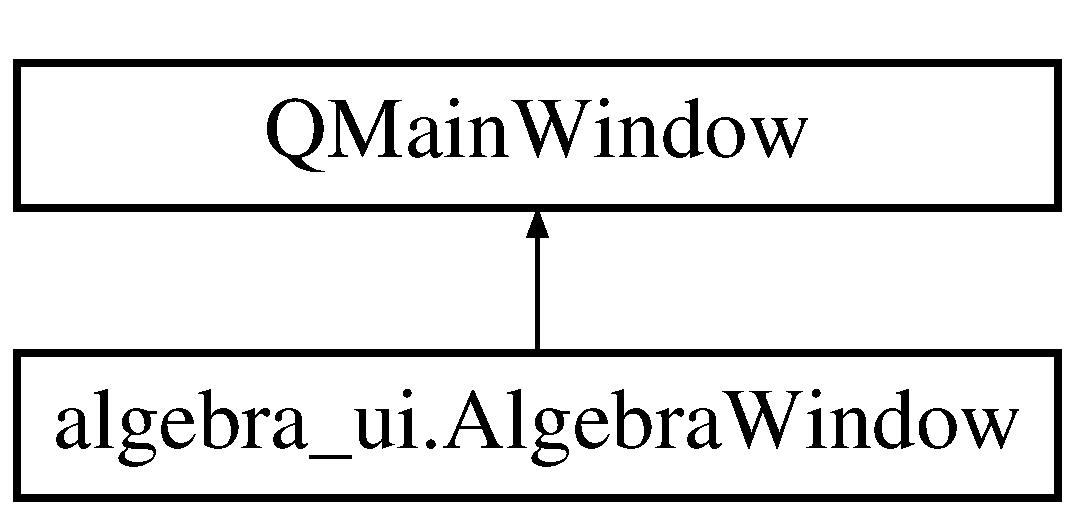
\includegraphics[height=2.000000cm]{classalgebra__ui_1_1_algebra_window}
\end{center}
\end{figure}
\subsection*{Public Member Functions}
\begin{DoxyCompactItemize}
\item 
def \hyperlink{classalgebra__ui_1_1_algebra_window_a8a5c82431399cd2792b44fdcff991873}{\+\_\+\+\_\+init\+\_\+\+\_\+} (self, path=\char`\"{}\char`\"{})
\begin{DoxyCompactList}\small\item\em The constructor of the Algebra window. \end{DoxyCompactList}\end{DoxyCompactItemize}
\subsection*{Public Attributes}
\begin{DoxyCompactItemize}
\item 
\mbox{\Hypertarget{classalgebra__ui_1_1_algebra_window_ae16b0dcdab0a23dcd7e70c9393a237f8}\label{classalgebra__ui_1_1_algebra_window_ae16b0dcdab0a23dcd7e70c9393a237f8}} 
{\bfseries path}
\item 
\mbox{\Hypertarget{classalgebra__ui_1_1_algebra_window_ab1e51746684b78e3f212c021727e2eeb}\label{classalgebra__ui_1_1_algebra_window_ab1e51746684b78e3f212c021727e2eeb}} 
{\bfseries xpath}
\item 
\mbox{\Hypertarget{classalgebra__ui_1_1_algebra_window_ada16e7befcac57d298e6ff6ea809c04f}\label{classalgebra__ui_1_1_algebra_window_ada16e7befcac57d298e6ff6ea809c04f}} 
{\bfseries slope1}
\item 
\mbox{\Hypertarget{classalgebra__ui_1_1_algebra_window_acdb30e012617d014d4b7c58c157d1472}\label{classalgebra__ui_1_1_algebra_window_acdb30e012617d014d4b7c58c157d1472}} 
{\bfseries slope2}
\item 
\mbox{\Hypertarget{classalgebra__ui_1_1_algebra_window_af928f66e8c1f01f3a3131db1f371608b}\label{classalgebra__ui_1_1_algebra_window_af928f66e8c1f01f3a3131db1f371608b}} 
{\bfseries pytha}
\end{DoxyCompactItemize}


\subsection{Detailed Description}
\hyperlink{classalgebra__ui_1_1_algebra_window}{Algebra\+Window} is a class that implements the G\+UI components for the Algebra operation menu. 

\subsection{Constructor \& Destructor Documentation}
\mbox{\Hypertarget{classalgebra__ui_1_1_algebra_window_a8a5c82431399cd2792b44fdcff991873}\label{classalgebra__ui_1_1_algebra_window_a8a5c82431399cd2792b44fdcff991873}} 
\index{algebra\+\_\+ui\+::\+Algebra\+Window@{algebra\+\_\+ui\+::\+Algebra\+Window}!\+\_\+\+\_\+init\+\_\+\+\_\+@{\+\_\+\+\_\+init\+\_\+\+\_\+}}
\index{\+\_\+\+\_\+init\+\_\+\+\_\+@{\+\_\+\+\_\+init\+\_\+\+\_\+}!algebra\+\_\+ui\+::\+Algebra\+Window@{algebra\+\_\+ui\+::\+Algebra\+Window}}
\subsubsection{\texorpdfstring{\+\_\+\+\_\+init\+\_\+\+\_\+()}{\_\_init\_\_()}}
{\footnotesize\ttfamily def algebra\+\_\+ui.\+Algebra\+Window.\+\_\+\+\_\+init\+\_\+\+\_\+ (\begin{DoxyParamCaption}\item[{}]{self,  }\item[{}]{path = {\ttfamily \char`\"{}\char`\"{}} }\end{DoxyParamCaption})}



The constructor of the Algebra window. 

Creates a pop up window that displays and sets up the buttons that are necessary to navigate from the Algebra window to other parts of the application. Also sets up the Algebra window according to the created style sheet. 
\begin{DoxyParams}{Parameters}
{\em path} & The current path on which the file is found. Default value is an empty path. \\
\hline
\end{DoxyParams}


The documentation for this class was generated from the following file\+:\begin{DoxyCompactItemize}
\item 
src/uis/\hyperlink{algebra__ui_8py}{algebra\+\_\+ui.\+py}\end{DoxyCompactItemize}

\hypertarget{classarea__ui_1_1_area_window}{}\section{area\+\_\+ui.\+Area\+Window Class Reference}
\label{classarea__ui_1_1_area_window}\index{area\+\_\+ui.\+Area\+Window@{area\+\_\+ui.\+Area\+Window}}


\hyperlink{classarea__ui_1_1_area_window}{Area\+Window} is a class that implements the G\+UI components for the Area operation.  


Inheritance diagram for area\+\_\+ui.\+Area\+Window\+:\begin{figure}[H]
\begin{center}
\leavevmode
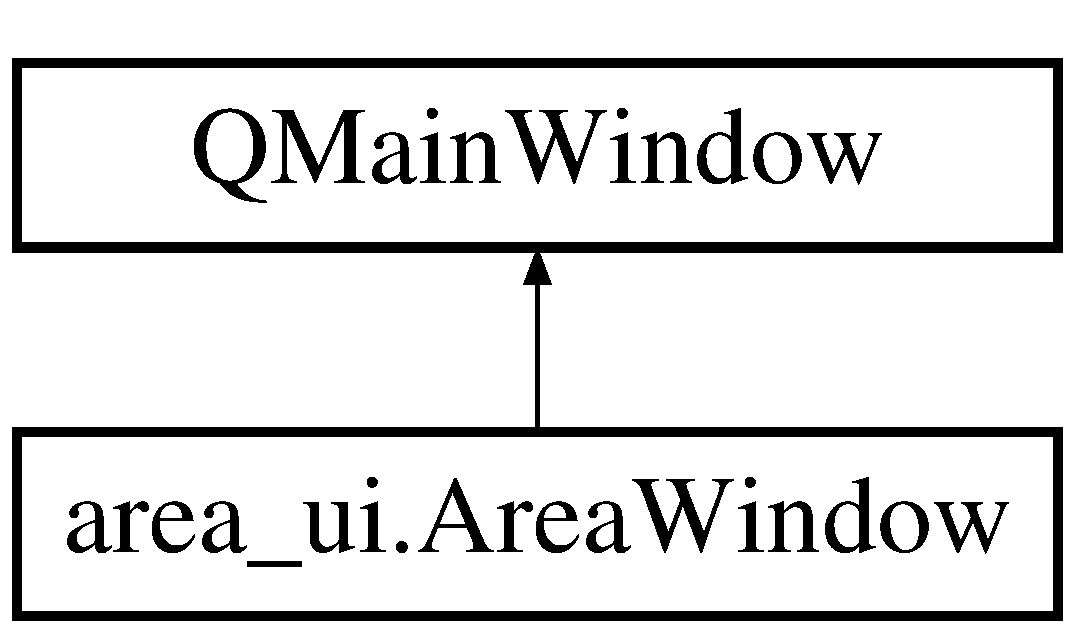
\includegraphics[height=2.000000cm]{classarea__ui_1_1_area_window}
\end{center}
\end{figure}
\subsection*{Public Member Functions}
\begin{DoxyCompactItemize}
\item 
def \hyperlink{classarea__ui_1_1_area_window_a4147cce2b2137dde0a7ac73901b8d9a4}{\+\_\+\+\_\+init\+\_\+\+\_\+} (self, path=\char`\"{}\char`\"{})
\begin{DoxyCompactList}\small\item\em The constructor of the Area window. \end{DoxyCompactList}\item 
def \hyperlink{classarea__ui_1_1_area_window_af95844b38370da348b28e9b1238467ad}{area} (self)
\begin{DoxyCompactList}\small\item\em Displays the area of selected shape given appropriate side lengths/radius. \end{DoxyCompactList}\end{DoxyCompactItemize}
\subsection*{Public Attributes}
\begin{DoxyCompactItemize}
\item 
\mbox{\Hypertarget{classarea__ui_1_1_area_window_a78ffcbed4656d6e098b73228423db2f8}\label{classarea__ui_1_1_area_window_a78ffcbed4656d6e098b73228423db2f8}} 
{\bfseries path}
\end{DoxyCompactItemize}


\subsection{Detailed Description}
\hyperlink{classarea__ui_1_1_area_window}{Area\+Window} is a class that implements the G\+UI components for the Area operation. 

\subsection{Constructor \& Destructor Documentation}
\mbox{\Hypertarget{classarea__ui_1_1_area_window_a4147cce2b2137dde0a7ac73901b8d9a4}\label{classarea__ui_1_1_area_window_a4147cce2b2137dde0a7ac73901b8d9a4}} 
\index{area\+\_\+ui\+::\+Area\+Window@{area\+\_\+ui\+::\+Area\+Window}!\+\_\+\+\_\+init\+\_\+\+\_\+@{\+\_\+\+\_\+init\+\_\+\+\_\+}}
\index{\+\_\+\+\_\+init\+\_\+\+\_\+@{\+\_\+\+\_\+init\+\_\+\+\_\+}!area\+\_\+ui\+::\+Area\+Window@{area\+\_\+ui\+::\+Area\+Window}}
\subsubsection{\texorpdfstring{\+\_\+\+\_\+init\+\_\+\+\_\+()}{\_\_init\_\_()}}
{\footnotesize\ttfamily def area\+\_\+ui.\+Area\+Window.\+\_\+\+\_\+init\+\_\+\+\_\+ (\begin{DoxyParamCaption}\item[{}]{self,  }\item[{}]{path = {\ttfamily \char`\"{}\char`\"{}} }\end{DoxyParamCaption})}



The constructor of the Area window. 

Creates a pop up window that displays and sets up the buttons and input fields that are necessary to obtain input from the user and calculate the appropriate answer. Also sets up the window according to the created style sheet. 
\begin{DoxyParams}{Parameters}
{\em path} & The current path on which the file is found. Default value is an empty path. \\
\hline
\end{DoxyParams}


\subsection{Member Function Documentation}
\mbox{\Hypertarget{classarea__ui_1_1_area_window_af95844b38370da348b28e9b1238467ad}\label{classarea__ui_1_1_area_window_af95844b38370da348b28e9b1238467ad}} 
\index{area\+\_\+ui\+::\+Area\+Window@{area\+\_\+ui\+::\+Area\+Window}!area@{area}}
\index{area@{area}!area\+\_\+ui\+::\+Area\+Window@{area\+\_\+ui\+::\+Area\+Window}}
\subsubsection{\texorpdfstring{area()}{area()}}
{\footnotesize\ttfamily def area\+\_\+ui.\+Area\+Window.\+area (\begin{DoxyParamCaption}\item[{}]{self }\end{DoxyParamCaption})}



Displays the area of selected shape given appropriate side lengths/radius. 

Takes in up to 3 side lengths and a radius as input from the user through input fields, and shows the user the result on the window 

The documentation for this class was generated from the following file\+:\begin{DoxyCompactItemize}
\item 
src/uis/\hyperlink{area__ui_8py}{area\+\_\+ui.\+py}\end{DoxyCompactItemize}

\hypertarget{class_body_fat__ui_1_1_b_f_window}{}\section{Body\+Fat\+\_\+ui.\+B\+F\+Window Class Reference}
\label{class_body_fat__ui_1_1_b_f_window}\index{Body\+Fat\+\_\+ui.\+B\+F\+Window@{Body\+Fat\+\_\+ui.\+B\+F\+Window}}


\hyperlink{class_body_fat__ui_1_1_b_f_window}{B\+F\+Window} is a class that implements the G\+UI components for the Body Fat operation.  


Inheritance diagram for Body\+Fat\+\_\+ui.\+B\+F\+Window\+:\begin{figure}[H]
\begin{center}
\leavevmode
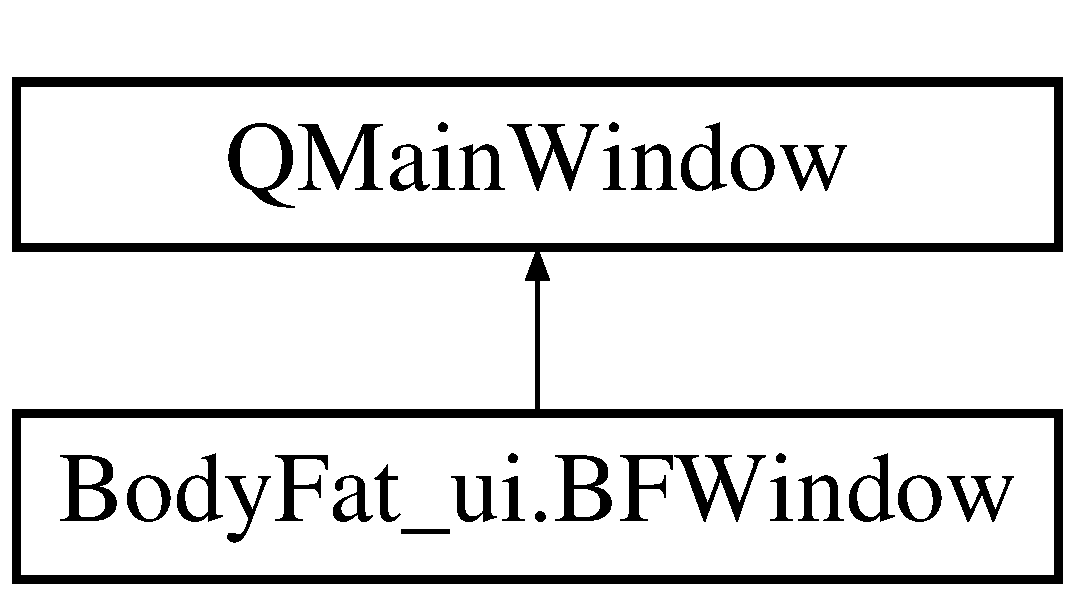
\includegraphics[height=2.000000cm]{class_body_fat__ui_1_1_b_f_window}
\end{center}
\end{figure}
\subsection*{Public Member Functions}
\begin{DoxyCompactItemize}
\item 
def \hyperlink{class_body_fat__ui_1_1_b_f_window_a3ee0d136b0b25e045fd9a8a6356819b1}{\+\_\+\+\_\+init\+\_\+\+\_\+} (self, path=\char`\"{}\char`\"{})
\begin{DoxyCompactList}\small\item\em The constructor of the Body Fat window. \end{DoxyCompactList}\item 
def \hyperlink{class_body_fat__ui_1_1_b_f_window_a1c3b98d97dc41255235c5e739980b16f}{bf} (self)
\begin{DoxyCompactList}\small\item\em Displays the Body Fat rating and its meaning based on the metrics the user provides. \end{DoxyCompactList}\item 
\mbox{\Hypertarget{class_body_fat__ui_1_1_b_f_window_a25e504f2540df47b7c81d7febf5eeec2}\label{class_body_fat__ui_1_1_b_f_window_a25e504f2540df47b7c81d7febf5eeec2}} 
def \hyperlink{class_body_fat__ui_1_1_b_f_window_a25e504f2540df47b7c81d7febf5eeec2}{close\+Event} (self, event)
\begin{DoxyCompactList}\small\item\em Resets fields and closes window. \end{DoxyCompactList}\item 
\mbox{\Hypertarget{class_body_fat__ui_1_1_b_f_window_a24594a009a7f736a732253c4d7304c24}\label{class_body_fat__ui_1_1_b_f_window_a24594a009a7f736a732253c4d7304c24}} 
def \hyperlink{class_body_fat__ui_1_1_b_f_window_a24594a009a7f736a732253c4d7304c24}{clear\+Fields} (self)
\begin{DoxyCompactList}\small\item\em Clears all input and output fields. \end{DoxyCompactList}\end{DoxyCompactItemize}
\subsection*{Public Attributes}
\begin{DoxyCompactItemize}
\item 
\mbox{\Hypertarget{class_body_fat__ui_1_1_b_f_window_a22747b4a05d316e1ac4d9421051427b5}\label{class_body_fat__ui_1_1_b_f_window_a22747b4a05d316e1ac4d9421051427b5}} 
{\bfseries path}
\end{DoxyCompactItemize}


\subsection{Detailed Description}
\hyperlink{class_body_fat__ui_1_1_b_f_window}{B\+F\+Window} is a class that implements the G\+UI components for the Body Fat operation. 

\subsection{Constructor \& Destructor Documentation}
\mbox{\Hypertarget{class_body_fat__ui_1_1_b_f_window_a3ee0d136b0b25e045fd9a8a6356819b1}\label{class_body_fat__ui_1_1_b_f_window_a3ee0d136b0b25e045fd9a8a6356819b1}} 
\index{Body\+Fat\+\_\+ui\+::\+B\+F\+Window@{Body\+Fat\+\_\+ui\+::\+B\+F\+Window}!\+\_\+\+\_\+init\+\_\+\+\_\+@{\+\_\+\+\_\+init\+\_\+\+\_\+}}
\index{\+\_\+\+\_\+init\+\_\+\+\_\+@{\+\_\+\+\_\+init\+\_\+\+\_\+}!Body\+Fat\+\_\+ui\+::\+B\+F\+Window@{Body\+Fat\+\_\+ui\+::\+B\+F\+Window}}
\subsubsection{\texorpdfstring{\+\_\+\+\_\+init\+\_\+\+\_\+()}{\_\_init\_\_()}}
{\footnotesize\ttfamily def Body\+Fat\+\_\+ui.\+B\+F\+Window.\+\_\+\+\_\+init\+\_\+\+\_\+ (\begin{DoxyParamCaption}\item[{}]{self,  }\item[{}]{path = {\ttfamily \char`\"{}\char`\"{}} }\end{DoxyParamCaption})}



The constructor of the Body Fat window. 

Creates a pop up window that displays and sets up the buttons and input fields that are necessary to obtain input from the user and calculate the appropriate answer. Also sets up the window according to the created style sheet. 
\begin{DoxyParams}{Parameters}
{\em path} & The current path on which the file is found. Default value is an empty path. \\
\hline
\end{DoxyParams}


\subsection{Member Function Documentation}
\mbox{\Hypertarget{class_body_fat__ui_1_1_b_f_window_a1c3b98d97dc41255235c5e739980b16f}\label{class_body_fat__ui_1_1_b_f_window_a1c3b98d97dc41255235c5e739980b16f}} 
\index{Body\+Fat\+\_\+ui\+::\+B\+F\+Window@{Body\+Fat\+\_\+ui\+::\+B\+F\+Window}!bf@{bf}}
\index{bf@{bf}!Body\+Fat\+\_\+ui\+::\+B\+F\+Window@{Body\+Fat\+\_\+ui\+::\+B\+F\+Window}}
\subsubsection{\texorpdfstring{bf()}{bf()}}
{\footnotesize\ttfamily def Body\+Fat\+\_\+ui.\+B\+F\+Window.\+bf (\begin{DoxyParamCaption}\item[{}]{self }\end{DoxyParamCaption})}



Displays the Body Fat rating and its meaning based on the metrics the user provides. 

Takes in age, gender, height, and weight from the user through input fields, and shows the user the result on the window 

The documentation for this class was generated from the following file\+:\begin{DoxyCompactItemize}
\item 
src/uis/\hyperlink{_body_fat__ui_8py}{Body\+Fat\+\_\+ui.\+py}\end{DoxyCompactItemize}

\hypertarget{classbinary__arithmetic__ui_1_1_bin_arithmetic_window}{}\section{binary\+\_\+arithmetic\+\_\+ui.\+Bin\+Arithmetic\+Window Class Reference}
\label{classbinary__arithmetic__ui_1_1_bin_arithmetic_window}\index{binary\+\_\+arithmetic\+\_\+ui.\+Bin\+Arithmetic\+Window@{binary\+\_\+arithmetic\+\_\+ui.\+Bin\+Arithmetic\+Window}}


\hyperlink{classbinary__arithmetic__ui_1_1_bin_arithmetic_window}{Bin\+Arithmetic\+Window} is a class that implements the G\+UI components for the Binary Arithmetic operations.  


Inheritance diagram for binary\+\_\+arithmetic\+\_\+ui.\+Bin\+Arithmetic\+Window\+:\begin{figure}[H]
\begin{center}
\leavevmode
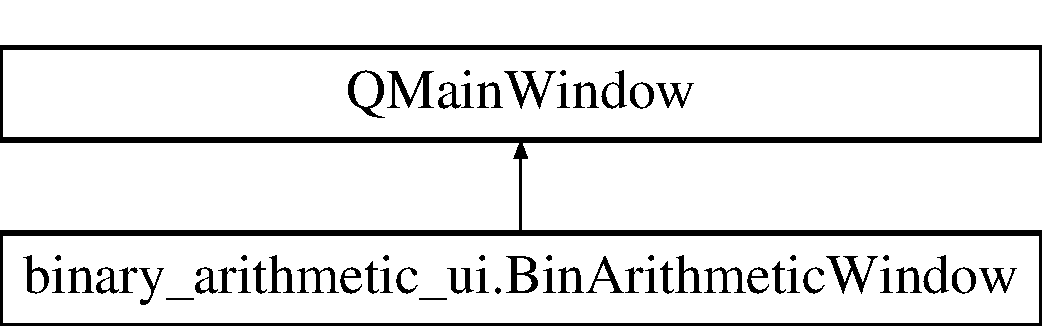
\includegraphics[height=2.000000cm]{classbinary__arithmetic__ui_1_1_bin_arithmetic_window}
\end{center}
\end{figure}
\subsection*{Public Member Functions}
\begin{DoxyCompactItemize}
\item 
def \hyperlink{classbinary__arithmetic__ui_1_1_bin_arithmetic_window_a0511ad3ac87d51b48420f7dc4c4dd35d}{\+\_\+\+\_\+init\+\_\+\+\_\+} (self, path=\char`\"{}\char`\"{})
\begin{DoxyCompactList}\small\item\em The constructor of the Binary Arithmetic window. \end{DoxyCompactList}\item 
def \hyperlink{classbinary__arithmetic__ui_1_1_bin_arithmetic_window_ae3a5ab3baee92929acc1ee524456825a}{bin\+Arithmetic} (self)
\begin{DoxyCompactList}\small\item\em Displays the arithmetic output of two binary numbers using various operators. \end{DoxyCompactList}\end{DoxyCompactItemize}
\subsection*{Public Attributes}
\begin{DoxyCompactItemize}
\item 
\mbox{\Hypertarget{classbinary__arithmetic__ui_1_1_bin_arithmetic_window_a33ebbcf56fc1406f4569f8db705c5dab}\label{classbinary__arithmetic__ui_1_1_bin_arithmetic_window_a33ebbcf56fc1406f4569f8db705c5dab}} 
{\bfseries path}
\end{DoxyCompactItemize}


\subsection{Detailed Description}
\hyperlink{classbinary__arithmetic__ui_1_1_bin_arithmetic_window}{Bin\+Arithmetic\+Window} is a class that implements the G\+UI components for the Binary Arithmetic operations. 

\subsection{Constructor \& Destructor Documentation}
\mbox{\Hypertarget{classbinary__arithmetic__ui_1_1_bin_arithmetic_window_a0511ad3ac87d51b48420f7dc4c4dd35d}\label{classbinary__arithmetic__ui_1_1_bin_arithmetic_window_a0511ad3ac87d51b48420f7dc4c4dd35d}} 
\index{binary\+\_\+arithmetic\+\_\+ui\+::\+Bin\+Arithmetic\+Window@{binary\+\_\+arithmetic\+\_\+ui\+::\+Bin\+Arithmetic\+Window}!\+\_\+\+\_\+init\+\_\+\+\_\+@{\+\_\+\+\_\+init\+\_\+\+\_\+}}
\index{\+\_\+\+\_\+init\+\_\+\+\_\+@{\+\_\+\+\_\+init\+\_\+\+\_\+}!binary\+\_\+arithmetic\+\_\+ui\+::\+Bin\+Arithmetic\+Window@{binary\+\_\+arithmetic\+\_\+ui\+::\+Bin\+Arithmetic\+Window}}
\subsubsection{\texorpdfstring{\+\_\+\+\_\+init\+\_\+\+\_\+()}{\_\_init\_\_()}}
{\footnotesize\ttfamily def binary\+\_\+arithmetic\+\_\+ui.\+Bin\+Arithmetic\+Window.\+\_\+\+\_\+init\+\_\+\+\_\+ (\begin{DoxyParamCaption}\item[{}]{self,  }\item[{}]{path = {\ttfamily \char`\"{}\char`\"{}} }\end{DoxyParamCaption})}



The constructor of the Binary Arithmetic window. 

Creates a pop up window that displays and sets up the buttons and input fields that are necessary to obtain input from the user and calculate the appropriate answer. Also sets up the window according to the created style sheet. 
\begin{DoxyParams}{Parameters}
{\em path} & The current path on which the file is found. Default value is an empty path. \\
\hline
\end{DoxyParams}


\subsection{Member Function Documentation}
\mbox{\Hypertarget{classbinary__arithmetic__ui_1_1_bin_arithmetic_window_ae3a5ab3baee92929acc1ee524456825a}\label{classbinary__arithmetic__ui_1_1_bin_arithmetic_window_ae3a5ab3baee92929acc1ee524456825a}} 
\index{binary\+\_\+arithmetic\+\_\+ui\+::\+Bin\+Arithmetic\+Window@{binary\+\_\+arithmetic\+\_\+ui\+::\+Bin\+Arithmetic\+Window}!bin\+Arithmetic@{bin\+Arithmetic}}
\index{bin\+Arithmetic@{bin\+Arithmetic}!binary\+\_\+arithmetic\+\_\+ui\+::\+Bin\+Arithmetic\+Window@{binary\+\_\+arithmetic\+\_\+ui\+::\+Bin\+Arithmetic\+Window}}
\subsubsection{\texorpdfstring{bin\+Arithmetic()}{binArithmetic()}}
{\footnotesize\ttfamily def binary\+\_\+arithmetic\+\_\+ui.\+Bin\+Arithmetic\+Window.\+bin\+Arithmetic (\begin{DoxyParamCaption}\item[{}]{self }\end{DoxyParamCaption})}



Displays the arithmetic output of two binary numbers using various operators. 

Takes in two binary numbers and the operator from the user through input fields, and shows the user the result on the window 

The documentation for this class was generated from the following file\+:\begin{DoxyCompactItemize}
\item 
src/uis/\hyperlink{binary__arithmetic__ui_8py}{binary\+\_\+arithmetic\+\_\+ui.\+py}\end{DoxyCompactItemize}

\hypertarget{classbinary__ui_1_1_binary_window}{}\section{binary\+\_\+ui.\+Binary\+Window Class Reference}
\label{classbinary__ui_1_1_binary_window}\index{binary\+\_\+ui.\+Binary\+Window@{binary\+\_\+ui.\+Binary\+Window}}


\hyperlink{classbinary__ui_1_1_binary_window}{Binary\+Window} is a class that implements the G\+UI components for the Binary operation menu.  


Inheritance diagram for binary\+\_\+ui.\+Binary\+Window\+:\begin{figure}[H]
\begin{center}
\leavevmode
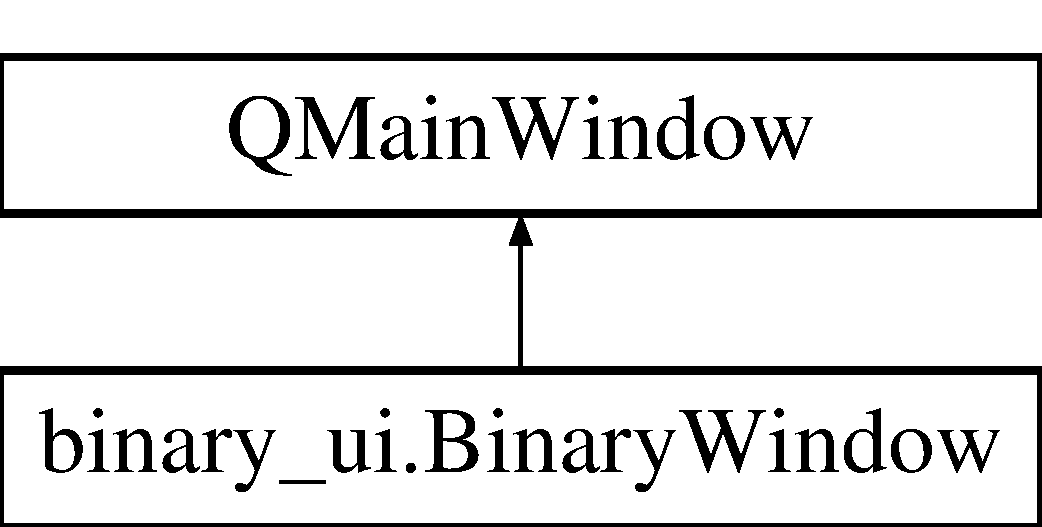
\includegraphics[height=2.000000cm]{classbinary__ui_1_1_binary_window}
\end{center}
\end{figure}
\subsection*{Public Member Functions}
\begin{DoxyCompactItemize}
\item 
def \hyperlink{classbinary__ui_1_1_binary_window_a2bc9146b516f338d24aa00087b8736bf}{\+\_\+\+\_\+init\+\_\+\+\_\+} (self, path=\char`\"{}\char`\"{})
\begin{DoxyCompactList}\small\item\em The constructor of the Binary window. \end{DoxyCompactList}\item 
\mbox{\Hypertarget{classbinary__ui_1_1_binary_window_a6d51e01a73e062679bab62190bacd085}\label{classbinary__ui_1_1_binary_window_a6d51e01a73e062679bab62190bacd085}} 
def \hyperlink{classbinary__ui_1_1_binary_window_a6d51e01a73e062679bab62190bacd085}{close\+Event} (self, event)
\begin{DoxyCompactList}\small\item\em Closes the window and any other geometry operation windows. \end{DoxyCompactList}\end{DoxyCompactItemize}
\subsection*{Public Attributes}
\begin{DoxyCompactItemize}
\item 
\mbox{\Hypertarget{classbinary__ui_1_1_binary_window_a503e75da778a99d49bb4e881104c51c8}\label{classbinary__ui_1_1_binary_window_a503e75da778a99d49bb4e881104c51c8}} 
{\bfseries path}
\item 
\mbox{\Hypertarget{classbinary__ui_1_1_binary_window_a1eb2477c8aef7283a71a03fec0d227fa}\label{classbinary__ui_1_1_binary_window_a1eb2477c8aef7283a71a03fec0d227fa}} 
{\bfseries xpath}
\item 
\mbox{\Hypertarget{classbinary__ui_1_1_binary_window_a35f478bed69ae16b900d8a68439f2ee2}\label{classbinary__ui_1_1_binary_window_a35f478bed69ae16b900d8a68439f2ee2}} 
{\bfseries fp}
\item 
\mbox{\Hypertarget{classbinary__ui_1_1_binary_window_a43cd237b6ac8533d8996144e687877cf}\label{classbinary__ui_1_1_binary_window_a43cd237b6ac8533d8996144e687877cf}} 
{\bfseries ba}
\item 
\mbox{\Hypertarget{classbinary__ui_1_1_binary_window_a7904b3d4e6281944838e25000b3ba0e6}\label{classbinary__ui_1_1_binary_window_a7904b3d4e6281944838e25000b3ba0e6}} 
{\bfseries bw}
\end{DoxyCompactItemize}


\subsection{Detailed Description}
\hyperlink{classbinary__ui_1_1_binary_window}{Binary\+Window} is a class that implements the G\+UI components for the Binary operation menu. 

\subsection{Constructor \& Destructor Documentation}
\mbox{\Hypertarget{classbinary__ui_1_1_binary_window_a2bc9146b516f338d24aa00087b8736bf}\label{classbinary__ui_1_1_binary_window_a2bc9146b516f338d24aa00087b8736bf}} 
\index{binary\+\_\+ui\+::\+Binary\+Window@{binary\+\_\+ui\+::\+Binary\+Window}!\+\_\+\+\_\+init\+\_\+\+\_\+@{\+\_\+\+\_\+init\+\_\+\+\_\+}}
\index{\+\_\+\+\_\+init\+\_\+\+\_\+@{\+\_\+\+\_\+init\+\_\+\+\_\+}!binary\+\_\+ui\+::\+Binary\+Window@{binary\+\_\+ui\+::\+Binary\+Window}}
\subsubsection{\texorpdfstring{\+\_\+\+\_\+init\+\_\+\+\_\+()}{\_\_init\_\_()}}
{\footnotesize\ttfamily def binary\+\_\+ui.\+Binary\+Window.\+\_\+\+\_\+init\+\_\+\+\_\+ (\begin{DoxyParamCaption}\item[{}]{self,  }\item[{}]{path = {\ttfamily \char`\"{}\char`\"{}} }\end{DoxyParamCaption})}



The constructor of the Binary window. 

Creates a pop up window that displays and sets up the buttons that are necessary to navigate from the Binary window to other parts of the application. Also sets up the Binary window according to the created style sheet. 
\begin{DoxyParams}{Parameters}
{\em path} & The current path on which the file is found. Default value is an empty path. \\
\hline
\end{DoxyParams}


The documentation for this class was generated from the following file\+:\begin{DoxyCompactItemize}
\item 
src/uis/\hyperlink{binary__ui_8py}{binary\+\_\+ui.\+py}\end{DoxyCompactItemize}

\hypertarget{classbitwise__ui_1_1_bitwise_window}{}\section{bitwise\+\_\+ui.\+Bitwise\+Window Class Reference}
\label{classbitwise__ui_1_1_bitwise_window}\index{bitwise\+\_\+ui.\+Bitwise\+Window@{bitwise\+\_\+ui.\+Bitwise\+Window}}


\hyperlink{classbitwise__ui_1_1_bitwise_window}{Bitwise\+Window} is a class that implements the G\+UI components for the Bitwise operations.  


Inheritance diagram for bitwise\+\_\+ui.\+Bitwise\+Window\+:\begin{figure}[H]
\begin{center}
\leavevmode
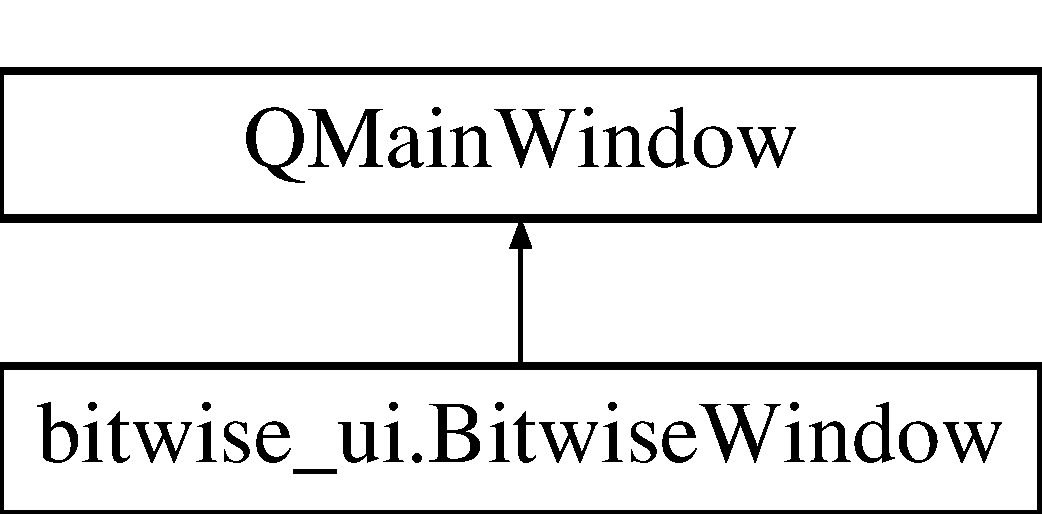
\includegraphics[height=2.000000cm]{classbitwise__ui_1_1_bitwise_window}
\end{center}
\end{figure}
\subsection*{Public Member Functions}
\begin{DoxyCompactItemize}
\item 
def \hyperlink{classbitwise__ui_1_1_bitwise_window_a5f91a64a61e0cd5282e40925c4417171}{\+\_\+\+\_\+init\+\_\+\+\_\+} (self, path=\char`\"{}\char`\"{})
\begin{DoxyCompactList}\small\item\em The constructor of the Bitwise window. \end{DoxyCompactList}\item 
def \hyperlink{classbitwise__ui_1_1_bitwise_window_a3eafe17fad0d129cd2bbab0d84e0e450}{bitwise} (self)
\begin{DoxyCompactList}\small\item\em Displays the output of bitwise operations on one or two binary numbers. \end{DoxyCompactList}\item 
\mbox{\Hypertarget{classbitwise__ui_1_1_bitwise_window_a1ff53a3a4a2ecbfe3bcf3b6485f4758e}\label{classbitwise__ui_1_1_bitwise_window_a1ff53a3a4a2ecbfe3bcf3b6485f4758e}} 
def \hyperlink{classbitwise__ui_1_1_bitwise_window_a1ff53a3a4a2ecbfe3bcf3b6485f4758e}{set\+Fields} (self)
\begin{DoxyCompactList}\small\item\em Changes and displays in text boxes corresponding to chosen operator. \end{DoxyCompactList}\item 
\mbox{\Hypertarget{classbitwise__ui_1_1_bitwise_window_a5fcf727d9271519cbe76fff538ff42b7}\label{classbitwise__ui_1_1_bitwise_window_a5fcf727d9271519cbe76fff538ff42b7}} 
def \hyperlink{classbitwise__ui_1_1_bitwise_window_a5fcf727d9271519cbe76fff538ff42b7}{close\+Event} (self, event)
\begin{DoxyCompactList}\small\item\em Closes window and clears inputs upon close. \end{DoxyCompactList}\item 
\mbox{\Hypertarget{classbitwise__ui_1_1_bitwise_window_a19e6fbad04a799221f0d29e689a14069}\label{classbitwise__ui_1_1_bitwise_window_a19e6fbad04a799221f0d29e689a14069}} 
def \hyperlink{classbitwise__ui_1_1_bitwise_window_a19e6fbad04a799221f0d29e689a14069}{clear\+Fields} (self)
\begin{DoxyCompactList}\small\item\em Clears all input and output fields. \end{DoxyCompactList}\end{DoxyCompactItemize}
\subsection*{Public Attributes}
\begin{DoxyCompactItemize}
\item 
\mbox{\Hypertarget{classbitwise__ui_1_1_bitwise_window_a50c5338d7eec89d033c090bd0efd525a}\label{classbitwise__ui_1_1_bitwise_window_a50c5338d7eec89d033c090bd0efd525a}} 
{\bfseries path}
\end{DoxyCompactItemize}


\subsection{Detailed Description}
\hyperlink{classbitwise__ui_1_1_bitwise_window}{Bitwise\+Window} is a class that implements the G\+UI components for the Bitwise operations. 

\subsection{Constructor \& Destructor Documentation}
\mbox{\Hypertarget{classbitwise__ui_1_1_bitwise_window_a5f91a64a61e0cd5282e40925c4417171}\label{classbitwise__ui_1_1_bitwise_window_a5f91a64a61e0cd5282e40925c4417171}} 
\index{bitwise\+\_\+ui\+::\+Bitwise\+Window@{bitwise\+\_\+ui\+::\+Bitwise\+Window}!\+\_\+\+\_\+init\+\_\+\+\_\+@{\+\_\+\+\_\+init\+\_\+\+\_\+}}
\index{\+\_\+\+\_\+init\+\_\+\+\_\+@{\+\_\+\+\_\+init\+\_\+\+\_\+}!bitwise\+\_\+ui\+::\+Bitwise\+Window@{bitwise\+\_\+ui\+::\+Bitwise\+Window}}
\subsubsection{\texorpdfstring{\+\_\+\+\_\+init\+\_\+\+\_\+()}{\_\_init\_\_()}}
{\footnotesize\ttfamily def bitwise\+\_\+ui.\+Bitwise\+Window.\+\_\+\+\_\+init\+\_\+\+\_\+ (\begin{DoxyParamCaption}\item[{}]{self,  }\item[{}]{path = {\ttfamily \char`\"{}\char`\"{}} }\end{DoxyParamCaption})}



The constructor of the Bitwise window. 

Creates a pop up window that displays and sets up the buttons and input fields that are necessary to obtain input from the user and calculate the appropriate answer. Also sets up the window according to the created style sheet. 
\begin{DoxyParams}{Parameters}
{\em path} & The current path on which the file is found. Default value is an empty path. \\
\hline
\end{DoxyParams}


\subsection{Member Function Documentation}
\mbox{\Hypertarget{classbitwise__ui_1_1_bitwise_window_a3eafe17fad0d129cd2bbab0d84e0e450}\label{classbitwise__ui_1_1_bitwise_window_a3eafe17fad0d129cd2bbab0d84e0e450}} 
\index{bitwise\+\_\+ui\+::\+Bitwise\+Window@{bitwise\+\_\+ui\+::\+Bitwise\+Window}!bitwise@{bitwise}}
\index{bitwise@{bitwise}!bitwise\+\_\+ui\+::\+Bitwise\+Window@{bitwise\+\_\+ui\+::\+Bitwise\+Window}}
\subsubsection{\texorpdfstring{bitwise()}{bitwise()}}
{\footnotesize\ttfamily def bitwise\+\_\+ui.\+Bitwise\+Window.\+bitwise (\begin{DoxyParamCaption}\item[{}]{self }\end{DoxyParamCaption})}



Displays the output of bitwise operations on one or two binary numbers. 

Takes in one or two binary numbers and the operator from the user through input fields, and shows the user the result on the window 

The documentation for this class was generated from the following file\+:\begin{DoxyCompactItemize}
\item 
src/uis/\hyperlink{bitwise__ui_8py}{bitwise\+\_\+ui.\+py}\end{DoxyCompactItemize}

\hypertarget{class_b_m_i__ui_1_1_b_m_i_window}{}\section{B\+M\+I\+\_\+ui.\+B\+M\+I\+Window Class Reference}
\label{class_b_m_i__ui_1_1_b_m_i_window}\index{B\+M\+I\+\_\+ui.\+B\+M\+I\+Window@{B\+M\+I\+\_\+ui.\+B\+M\+I\+Window}}


\hyperlink{class_b_m_i__ui_1_1_b_m_i_window}{B\+M\+I\+Window} is a class that implements the G\+UI components for the B\+MI operation.  


Inheritance diagram for B\+M\+I\+\_\+ui.\+B\+M\+I\+Window\+:\begin{figure}[H]
\begin{center}
\leavevmode
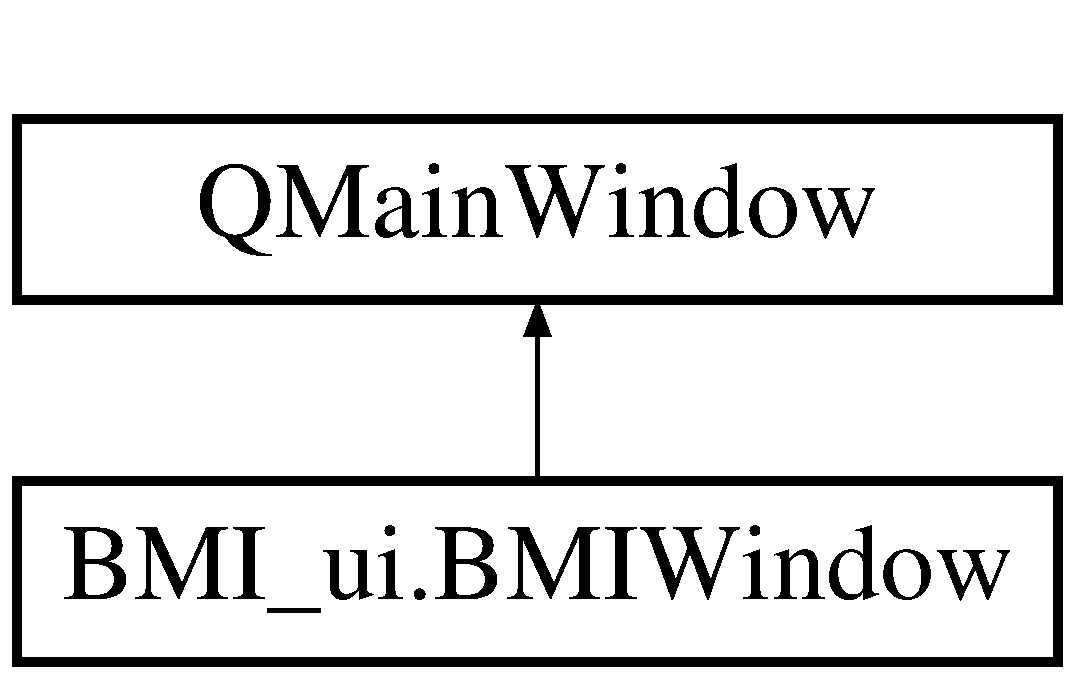
\includegraphics[height=2.000000cm]{class_b_m_i__ui_1_1_b_m_i_window}
\end{center}
\end{figure}
\subsection*{Public Member Functions}
\begin{DoxyCompactItemize}
\item 
def \hyperlink{class_b_m_i__ui_1_1_b_m_i_window_a0a248356e06771e32f78f0e7933d066f}{\+\_\+\+\_\+init\+\_\+\+\_\+} (self, path=\char`\"{}\char`\"{})
\begin{DoxyCompactList}\small\item\em The constructor of the B\+MI window. \end{DoxyCompactList}\item 
def \hyperlink{class_b_m_i__ui_1_1_b_m_i_window_ad8708c4a841a95a31c9f9d117f4440b2}{bmi} (self)
\begin{DoxyCompactList}\small\item\em Displays the B\+MI and its meaning based on the metrics the user provides. \end{DoxyCompactList}\end{DoxyCompactItemize}
\subsection*{Public Attributes}
\begin{DoxyCompactItemize}
\item 
\mbox{\Hypertarget{class_b_m_i__ui_1_1_b_m_i_window_a54aca672beae5ffa1e6e6eb51cefe459}\label{class_b_m_i__ui_1_1_b_m_i_window_a54aca672beae5ffa1e6e6eb51cefe459}} 
{\bfseries path}
\end{DoxyCompactItemize}


\subsection{Detailed Description}
\hyperlink{class_b_m_i__ui_1_1_b_m_i_window}{B\+M\+I\+Window} is a class that implements the G\+UI components for the B\+MI operation. 

\subsection{Constructor \& Destructor Documentation}
\mbox{\Hypertarget{class_b_m_i__ui_1_1_b_m_i_window_a0a248356e06771e32f78f0e7933d066f}\label{class_b_m_i__ui_1_1_b_m_i_window_a0a248356e06771e32f78f0e7933d066f}} 
\index{B\+M\+I\+\_\+ui\+::\+B\+M\+I\+Window@{B\+M\+I\+\_\+ui\+::\+B\+M\+I\+Window}!\+\_\+\+\_\+init\+\_\+\+\_\+@{\+\_\+\+\_\+init\+\_\+\+\_\+}}
\index{\+\_\+\+\_\+init\+\_\+\+\_\+@{\+\_\+\+\_\+init\+\_\+\+\_\+}!B\+M\+I\+\_\+ui\+::\+B\+M\+I\+Window@{B\+M\+I\+\_\+ui\+::\+B\+M\+I\+Window}}
\subsubsection{\texorpdfstring{\+\_\+\+\_\+init\+\_\+\+\_\+()}{\_\_init\_\_()}}
{\footnotesize\ttfamily def B\+M\+I\+\_\+ui.\+B\+M\+I\+Window.\+\_\+\+\_\+init\+\_\+\+\_\+ (\begin{DoxyParamCaption}\item[{}]{self,  }\item[{}]{path = {\ttfamily \char`\"{}\char`\"{}} }\end{DoxyParamCaption})}



The constructor of the B\+MI window. 

Creates a pop up window that displays and sets up the buttons and input fields that are necessary to obtain input from the user and calculate the appropriate answer. Also sets up the window according to the created style sheet. 
\begin{DoxyParams}{Parameters}
{\em path} & The current path on which the file is found. Default value is an empty path. \\
\hline
\end{DoxyParams}


\subsection{Member Function Documentation}
\mbox{\Hypertarget{class_b_m_i__ui_1_1_b_m_i_window_ad8708c4a841a95a31c9f9d117f4440b2}\label{class_b_m_i__ui_1_1_b_m_i_window_ad8708c4a841a95a31c9f9d117f4440b2}} 
\index{B\+M\+I\+\_\+ui\+::\+B\+M\+I\+Window@{B\+M\+I\+\_\+ui\+::\+B\+M\+I\+Window}!bmi@{bmi}}
\index{bmi@{bmi}!B\+M\+I\+\_\+ui\+::\+B\+M\+I\+Window@{B\+M\+I\+\_\+ui\+::\+B\+M\+I\+Window}}
\subsubsection{\texorpdfstring{bmi()}{bmi()}}
{\footnotesize\ttfamily def B\+M\+I\+\_\+ui.\+B\+M\+I\+Window.\+bmi (\begin{DoxyParamCaption}\item[{}]{self }\end{DoxyParamCaption})}



Displays the B\+MI and its meaning based on the metrics the user provides. 

Takes in height and weight from the user through input fields, and shows the user the result on the window 

The documentation for this class was generated from the following file\+:\begin{DoxyCompactItemize}
\item 
src/uis/\hyperlink{_b_m_i__ui_8py}{B\+M\+I\+\_\+ui.\+py}\end{DoxyCompactItemize}

\hypertarget{classmain__calculator_1_1_calculator}{}\section{main\+\_\+calculator.\+Calculator Class Reference}
\label{classmain__calculator_1_1_calculator}\index{main\+\_\+calculator.\+Calculator@{main\+\_\+calculator.\+Calculator}}


\hyperlink{classmain__calculator_1_1_calculator}{Calculator} is a class that implements the functionality of a basic calculator.  


\subsection*{Public Member Functions}
\begin{DoxyCompactItemize}
\item 
\mbox{\Hypertarget{classmain__calculator_1_1_calculator_a45a76b7d3db5c433160e9f54adcee065}\label{classmain__calculator_1_1_calculator_a45a76b7d3db5c433160e9f54adcee065}} 
def \hyperlink{classmain__calculator_1_1_calculator_a45a76b7d3db5c433160e9f54adcee065}{\+\_\+\+\_\+init\+\_\+\+\_\+} (self)
\begin{DoxyCompactList}\small\item\em The constructor of the \hyperlink{classmain__calculator_1_1_calculator}{Calculator}. \end{DoxyCompactList}\item 
\mbox{\Hypertarget{classmain__calculator_1_1_calculator_ab677caea0b75a1a1d42b08e853d16960}\label{classmain__calculator_1_1_calculator_ab677caea0b75a1a1d42b08e853d16960}} 
def \hyperlink{classmain__calculator_1_1_calculator_ab677caea0b75a1a1d42b08e853d16960}{get\+Curr\+Num} (self)
\begin{DoxyCompactList}\small\item\em Retreives current displayed number. \end{DoxyCompactList}\item 
def \hyperlink{classmain__calculator_1_1_calculator_a0e35cd11d7b3815e8158c0866686da02}{store\+Mem} (self)
\begin{DoxyCompactList}\small\item\em Stores the current number. \end{DoxyCompactList}\item 
def \hyperlink{classmain__calculator_1_1_calculator_affb70322f0ae2566a352414980fc4c76}{get\+Mem} (self)
\begin{DoxyCompactList}\small\item\em Displays current stored number. \end{DoxyCompactList}\item 
def \hyperlink{classmain__calculator_1_1_calculator_a9a9b05869e5fd1f5110bbe8d8005ba43}{value\+Input} (self, v)
\begin{DoxyCompactList}\small\item\em Display value of input. \end{DoxyCompactList}\item 
def \hyperlink{classmain__calculator_1_1_calculator_aac4299e4225a6aeeb11bc5410d900707}{reset} (self)
\begin{DoxyCompactList}\small\item\em Empty the line and current number stored. \end{DoxyCompactList}\item 
def \hyperlink{classmain__calculator_1_1_calculator_a7b20e7af5b1fdbd6061f6ea74b5b7a10}{addition} (self)
\begin{DoxyCompactList}\small\item\em Conducts calculator addition operation. \end{DoxyCompactList}\item 
def \hyperlink{classmain__calculator_1_1_calculator_a49813f25efdf28cf1ee41c9ffd6dd282}{subtraction} (self)
\begin{DoxyCompactList}\small\item\em Conducts calculator subtraction operation. \end{DoxyCompactList}\item 
def \hyperlink{classmain__calculator_1_1_calculator_a1358fbc08c2e9c60cb50f15c28649ffe}{multiplication} (self)
\begin{DoxyCompactList}\small\item\em Conducts calculator multiplication operation. \end{DoxyCompactList}\item 
def \hyperlink{classmain__calculator_1_1_calculator_a744ccd099c8deb999062579a9d8aa152}{power} (self)
\begin{DoxyCompactList}\small\item\em Conducts calculator power operation. \end{DoxyCompactList}\item 
def \hyperlink{classmain__calculator_1_1_calculator_acd2ea45d8a2e83dc8b2b0f555d972898}{division} (self)
\begin{DoxyCompactList}\small\item\em Conducts calculator division operation. \end{DoxyCompactList}\item 
def \hyperlink{classmain__calculator_1_1_calculator_ac64294792ca603503761632e96f811b7}{left\+\_\+bracket} (self)
\begin{DoxyCompactList}\small\item\em Adds left bracket operation. \end{DoxyCompactList}\item 
def \hyperlink{classmain__calculator_1_1_calculator_ae5a2100c17581ab6ed83b739a087f848}{right\+\_\+bracket} (self)
\begin{DoxyCompactList}\small\item\em Adds right bracket operation. \end{DoxyCompactList}\item 
\mbox{\Hypertarget{classmain__calculator_1_1_calculator_a96e33c57d1198a4c62f0a03205a5eef8}\label{classmain__calculator_1_1_calculator_a96e33c57d1198a4c62f0a03205a5eef8}} 
def \hyperlink{classmain__calculator_1_1_calculator_a96e33c57d1198a4c62f0a03205a5eef8}{evaluate} (self)
\begin{DoxyCompactList}\small\item\em Evaluates operation. \end{DoxyCompactList}\item 
\mbox{\Hypertarget{classmain__calculator_1_1_calculator_a40ee4c3e99a1ef96153a5492fda20a91}\label{classmain__calculator_1_1_calculator_a40ee4c3e99a1ef96153a5492fda20a91}} 
def \hyperlink{classmain__calculator_1_1_calculator_a40ee4c3e99a1ef96153a5492fda20a91}{delete} (self)
\begin{DoxyCompactList}\small\item\em Deletes entered input number by number. \end{DoxyCompactList}\end{DoxyCompactItemize}
\subsection*{Public Attributes}
\begin{DoxyCompactItemize}
\item 
\mbox{\Hypertarget{classmain__calculator_1_1_calculator_a6ac650245830a61eee1ad9a7f2270267}\label{classmain__calculator_1_1_calculator_a6ac650245830a61eee1ad9a7f2270267}} 
{\bfseries line\+Edit}
\item 
\mbox{\Hypertarget{classmain__calculator_1_1_calculator_a218561734fa0968bd494edbcdd326979}\label{classmain__calculator_1_1_calculator_a218561734fa0968bd494edbcdd326979}} 
{\bfseries curr\+Num}
\item 
\mbox{\Hypertarget{classmain__calculator_1_1_calculator_aef8b7f10a1c8302239a249ff5c1d360c}\label{classmain__calculator_1_1_calculator_aef8b7f10a1c8302239a249ff5c1d360c}} 
{\bfseries mem}
\end{DoxyCompactItemize}


\subsection{Detailed Description}
\hyperlink{classmain__calculator_1_1_calculator}{Calculator} is a class that implements the functionality of a basic calculator. 

\subsection{Member Function Documentation}
\mbox{\Hypertarget{classmain__calculator_1_1_calculator_a7b20e7af5b1fdbd6061f6ea74b5b7a10}\label{classmain__calculator_1_1_calculator_a7b20e7af5b1fdbd6061f6ea74b5b7a10}} 
\index{main\+\_\+calculator\+::\+Calculator@{main\+\_\+calculator\+::\+Calculator}!addition@{addition}}
\index{addition@{addition}!main\+\_\+calculator\+::\+Calculator@{main\+\_\+calculator\+::\+Calculator}}
\subsubsection{\texorpdfstring{addition()}{addition()}}
{\footnotesize\ttfamily def main\+\_\+calculator.\+Calculator.\+addition (\begin{DoxyParamCaption}\item[{}]{self }\end{DoxyParamCaption})}



Conducts calculator addition operation. 

Check if line input prior is not another operation and if it is not, display an empty string and adds an addition operation \mbox{\Hypertarget{classmain__calculator_1_1_calculator_acd2ea45d8a2e83dc8b2b0f555d972898}\label{classmain__calculator_1_1_calculator_acd2ea45d8a2e83dc8b2b0f555d972898}} 
\index{main\+\_\+calculator\+::\+Calculator@{main\+\_\+calculator\+::\+Calculator}!division@{division}}
\index{division@{division}!main\+\_\+calculator\+::\+Calculator@{main\+\_\+calculator\+::\+Calculator}}
\subsubsection{\texorpdfstring{division()}{division()}}
{\footnotesize\ttfamily def main\+\_\+calculator.\+Calculator.\+division (\begin{DoxyParamCaption}\item[{}]{self }\end{DoxyParamCaption})}



Conducts calculator division operation. 

Check if line input prior is not another operation and if it is not, display an empty string and adds a division operation \mbox{\Hypertarget{classmain__calculator_1_1_calculator_affb70322f0ae2566a352414980fc4c76}\label{classmain__calculator_1_1_calculator_affb70322f0ae2566a352414980fc4c76}} 
\index{main\+\_\+calculator\+::\+Calculator@{main\+\_\+calculator\+::\+Calculator}!get\+Mem@{get\+Mem}}
\index{get\+Mem@{get\+Mem}!main\+\_\+calculator\+::\+Calculator@{main\+\_\+calculator\+::\+Calculator}}
\subsubsection{\texorpdfstring{get\+Mem()}{getMem()}}
{\footnotesize\ttfamily def main\+\_\+calculator.\+Calculator.\+get\+Mem (\begin{DoxyParamCaption}\item[{}]{self }\end{DoxyParamCaption})}



Displays current stored number. 

Checks if current stored number is empty and adds new number number to store and display \mbox{\Hypertarget{classmain__calculator_1_1_calculator_ac64294792ca603503761632e96f811b7}\label{classmain__calculator_1_1_calculator_ac64294792ca603503761632e96f811b7}} 
\index{main\+\_\+calculator\+::\+Calculator@{main\+\_\+calculator\+::\+Calculator}!left\+\_\+bracket@{left\+\_\+bracket}}
\index{left\+\_\+bracket@{left\+\_\+bracket}!main\+\_\+calculator\+::\+Calculator@{main\+\_\+calculator\+::\+Calculator}}
\subsubsection{\texorpdfstring{left\+\_\+bracket()}{left\_bracket()}}
{\footnotesize\ttfamily def main\+\_\+calculator.\+Calculator.\+left\+\_\+bracket (\begin{DoxyParamCaption}\item[{}]{self }\end{DoxyParamCaption})}



Adds left bracket operation. 

Clears the display and adds a left bracket to the operation \mbox{\Hypertarget{classmain__calculator_1_1_calculator_a1358fbc08c2e9c60cb50f15c28649ffe}\label{classmain__calculator_1_1_calculator_a1358fbc08c2e9c60cb50f15c28649ffe}} 
\index{main\+\_\+calculator\+::\+Calculator@{main\+\_\+calculator\+::\+Calculator}!multiplication@{multiplication}}
\index{multiplication@{multiplication}!main\+\_\+calculator\+::\+Calculator@{main\+\_\+calculator\+::\+Calculator}}
\subsubsection{\texorpdfstring{multiplication()}{multiplication()}}
{\footnotesize\ttfamily def main\+\_\+calculator.\+Calculator.\+multiplication (\begin{DoxyParamCaption}\item[{}]{self }\end{DoxyParamCaption})}



Conducts calculator multiplication operation. 

Check if line input prior is not another operation and if it is not, display an empty string and adds a multiplication operation \mbox{\Hypertarget{classmain__calculator_1_1_calculator_a744ccd099c8deb999062579a9d8aa152}\label{classmain__calculator_1_1_calculator_a744ccd099c8deb999062579a9d8aa152}} 
\index{main\+\_\+calculator\+::\+Calculator@{main\+\_\+calculator\+::\+Calculator}!power@{power}}
\index{power@{power}!main\+\_\+calculator\+::\+Calculator@{main\+\_\+calculator\+::\+Calculator}}
\subsubsection{\texorpdfstring{power()}{power()}}
{\footnotesize\ttfamily def main\+\_\+calculator.\+Calculator.\+power (\begin{DoxyParamCaption}\item[{}]{self }\end{DoxyParamCaption})}



Conducts calculator power operation. 

Check if line input prior is not another operation and if it is not, display an empty string and adds a power operation \mbox{\Hypertarget{classmain__calculator_1_1_calculator_aac4299e4225a6aeeb11bc5410d900707}\label{classmain__calculator_1_1_calculator_aac4299e4225a6aeeb11bc5410d900707}} 
\index{main\+\_\+calculator\+::\+Calculator@{main\+\_\+calculator\+::\+Calculator}!reset@{reset}}
\index{reset@{reset}!main\+\_\+calculator\+::\+Calculator@{main\+\_\+calculator\+::\+Calculator}}
\subsubsection{\texorpdfstring{reset()}{reset()}}
{\footnotesize\ttfamily def main\+\_\+calculator.\+Calculator.\+reset (\begin{DoxyParamCaption}\item[{}]{self }\end{DoxyParamCaption})}



Empty the line and current number stored. 

Clears the line value and the current number value to an empty string value and display new blank value \mbox{\Hypertarget{classmain__calculator_1_1_calculator_ae5a2100c17581ab6ed83b739a087f848}\label{classmain__calculator_1_1_calculator_ae5a2100c17581ab6ed83b739a087f848}} 
\index{main\+\_\+calculator\+::\+Calculator@{main\+\_\+calculator\+::\+Calculator}!right\+\_\+bracket@{right\+\_\+bracket}}
\index{right\+\_\+bracket@{right\+\_\+bracket}!main\+\_\+calculator\+::\+Calculator@{main\+\_\+calculator\+::\+Calculator}}
\subsubsection{\texorpdfstring{right\+\_\+bracket()}{right\_bracket()}}
{\footnotesize\ttfamily def main\+\_\+calculator.\+Calculator.\+right\+\_\+bracket (\begin{DoxyParamCaption}\item[{}]{self }\end{DoxyParamCaption})}



Adds right bracket operation. 

Clears the display and adds a right bracket to the operation \mbox{\Hypertarget{classmain__calculator_1_1_calculator_a0e35cd11d7b3815e8158c0866686da02}\label{classmain__calculator_1_1_calculator_a0e35cd11d7b3815e8158c0866686da02}} 
\index{main\+\_\+calculator\+::\+Calculator@{main\+\_\+calculator\+::\+Calculator}!store\+Mem@{store\+Mem}}
\index{store\+Mem@{store\+Mem}!main\+\_\+calculator\+::\+Calculator@{main\+\_\+calculator\+::\+Calculator}}
\subsubsection{\texorpdfstring{store\+Mem()}{storeMem()}}
{\footnotesize\ttfamily def main\+\_\+calculator.\+Calculator.\+store\+Mem (\begin{DoxyParamCaption}\item[{}]{self }\end{DoxyParamCaption})}



Stores the current number. 

stores number for future use \mbox{\Hypertarget{classmain__calculator_1_1_calculator_a49813f25efdf28cf1ee41c9ffd6dd282}\label{classmain__calculator_1_1_calculator_a49813f25efdf28cf1ee41c9ffd6dd282}} 
\index{main\+\_\+calculator\+::\+Calculator@{main\+\_\+calculator\+::\+Calculator}!subtraction@{subtraction}}
\index{subtraction@{subtraction}!main\+\_\+calculator\+::\+Calculator@{main\+\_\+calculator\+::\+Calculator}}
\subsubsection{\texorpdfstring{subtraction()}{subtraction()}}
{\footnotesize\ttfamily def main\+\_\+calculator.\+Calculator.\+subtraction (\begin{DoxyParamCaption}\item[{}]{self }\end{DoxyParamCaption})}



Conducts calculator subtraction operation. 

Check if line input prior is not another operation and if it is not, display an empty string and adds a subtraction operation \mbox{\Hypertarget{classmain__calculator_1_1_calculator_a9a9b05869e5fd1f5110bbe8d8005ba43}\label{classmain__calculator_1_1_calculator_a9a9b05869e5fd1f5110bbe8d8005ba43}} 
\index{main\+\_\+calculator\+::\+Calculator@{main\+\_\+calculator\+::\+Calculator}!value\+Input@{value\+Input}}
\index{value\+Input@{value\+Input}!main\+\_\+calculator\+::\+Calculator@{main\+\_\+calculator\+::\+Calculator}}
\subsubsection{\texorpdfstring{value\+Input()}{valueInput()}}
{\footnotesize\ttfamily def main\+\_\+calculator.\+Calculator.\+value\+Input (\begin{DoxyParamCaption}\item[{}]{self,  }\item[{}]{v }\end{DoxyParamCaption})}



Display value of input. 

Adds the input v to the value of current number and displays it 

The documentation for this class was generated from the following file\+:\begin{DoxyCompactItemize}
\item 
src/uis/\+Calculators/\hyperlink{main__calculator_8py}{main\+\_\+calculator.\+py}\end{DoxyCompactItemize}

\hypertarget{class_conversion_base__ui_1_1_conversion_base_window}{}\section{Conversion\+Base\+\_\+ui.\+Conversion\+Base\+Window Class Reference}
\label{class_conversion_base__ui_1_1_conversion_base_window}\index{Conversion\+Base\+\_\+ui.\+Conversion\+Base\+Window@{Conversion\+Base\+\_\+ui.\+Conversion\+Base\+Window}}


\hyperlink{class_conversion_base__ui_1_1_conversion_base_window}{Conversion\+Base\+Window} is a class that implements the G\+UI components for the base conversion operation.  


Inheritance diagram for Conversion\+Base\+\_\+ui.\+Conversion\+Base\+Window\+:\begin{figure}[H]
\begin{center}
\leavevmode
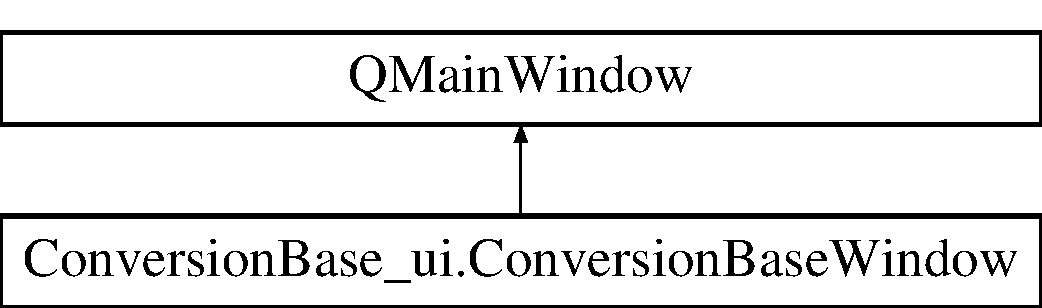
\includegraphics[height=2.000000cm]{class_conversion_base__ui_1_1_conversion_base_window}
\end{center}
\end{figure}
\subsection*{Public Member Functions}
\begin{DoxyCompactItemize}
\item 
def \hyperlink{class_conversion_base__ui_1_1_conversion_base_window_af8fe79c29cebc3c67c6260fe661872da}{\+\_\+\+\_\+init\+\_\+\+\_\+} (self, path=\char`\"{}\char`\"{})
\begin{DoxyCompactList}\small\item\em The constructor of the base conversion window. \end{DoxyCompactList}\item 
def \hyperlink{class_conversion_base__ui_1_1_conversion_base_window_af4bcf9d2cda570924af0efe9302f1c92}{baseconvert} (self)
\begin{DoxyCompactList}\small\item\em Displays the conversion a value of a base type 1 to a value of base type 2. \end{DoxyCompactList}\end{DoxyCompactItemize}
\subsection*{Public Attributes}
\begin{DoxyCompactItemize}
\item 
\mbox{\Hypertarget{class_conversion_base__ui_1_1_conversion_base_window_a1951c0b3099533052162596c673e0b3d}\label{class_conversion_base__ui_1_1_conversion_base_window_a1951c0b3099533052162596c673e0b3d}} 
{\bfseries path}
\end{DoxyCompactItemize}


\subsection{Detailed Description}
\hyperlink{class_conversion_base__ui_1_1_conversion_base_window}{Conversion\+Base\+Window} is a class that implements the G\+UI components for the base conversion operation. 

\subsection{Constructor \& Destructor Documentation}
\mbox{\Hypertarget{class_conversion_base__ui_1_1_conversion_base_window_af8fe79c29cebc3c67c6260fe661872da}\label{class_conversion_base__ui_1_1_conversion_base_window_af8fe79c29cebc3c67c6260fe661872da}} 
\index{Conversion\+Base\+\_\+ui\+::\+Conversion\+Base\+Window@{Conversion\+Base\+\_\+ui\+::\+Conversion\+Base\+Window}!\+\_\+\+\_\+init\+\_\+\+\_\+@{\+\_\+\+\_\+init\+\_\+\+\_\+}}
\index{\+\_\+\+\_\+init\+\_\+\+\_\+@{\+\_\+\+\_\+init\+\_\+\+\_\+}!Conversion\+Base\+\_\+ui\+::\+Conversion\+Base\+Window@{Conversion\+Base\+\_\+ui\+::\+Conversion\+Base\+Window}}
\subsubsection{\texorpdfstring{\+\_\+\+\_\+init\+\_\+\+\_\+()}{\_\_init\_\_()}}
{\footnotesize\ttfamily def Conversion\+Base\+\_\+ui.\+Conversion\+Base\+Window.\+\_\+\+\_\+init\+\_\+\+\_\+ (\begin{DoxyParamCaption}\item[{}]{self,  }\item[{}]{path = {\ttfamily \char`\"{}\char`\"{}} }\end{DoxyParamCaption})}



The constructor of the base conversion window. 

Creates a pop up window that displays and sets up the buttons and input fields that are necessary to obtain input from the user and calculate the appropriate answer. Also sets up the window according to the created style sheet. 
\begin{DoxyParams}{Parameters}
{\em path} & The current path on which the file is found. Default value is an empty path. \\
\hline
\end{DoxyParams}


\subsection{Member Function Documentation}
\mbox{\Hypertarget{class_conversion_base__ui_1_1_conversion_base_window_af4bcf9d2cda570924af0efe9302f1c92}\label{class_conversion_base__ui_1_1_conversion_base_window_af4bcf9d2cda570924af0efe9302f1c92}} 
\index{Conversion\+Base\+\_\+ui\+::\+Conversion\+Base\+Window@{Conversion\+Base\+\_\+ui\+::\+Conversion\+Base\+Window}!baseconvert@{baseconvert}}
\index{baseconvert@{baseconvert}!Conversion\+Base\+\_\+ui\+::\+Conversion\+Base\+Window@{Conversion\+Base\+\_\+ui\+::\+Conversion\+Base\+Window}}
\subsubsection{\texorpdfstring{baseconvert()}{baseconvert()}}
{\footnotesize\ttfamily def Conversion\+Base\+\_\+ui.\+Conversion\+Base\+Window.\+baseconvert (\begin{DoxyParamCaption}\item[{}]{self }\end{DoxyParamCaption})}



Displays the conversion a value of a base type 1 to a value of base type 2. 

Takes in 1 value and the convert to and convert from type as input from the user through input fields and shows the user the result on the window 

The documentation for this class was generated from the following file\+:\begin{DoxyCompactItemize}
\item 
src/uis/\hyperlink{_conversion_base__ui_8py}{Conversion\+Base\+\_\+ui.\+py}\end{DoxyCompactItemize}

\hypertarget{class_conversion_crypto__ui_1_1_conversion_crypto_window}{}\section{Conversion\+Crypto\+\_\+ui.\+Conversion\+Crypto\+Window Class Reference}
\label{class_conversion_crypto__ui_1_1_conversion_crypto_window}\index{Conversion\+Crypto\+\_\+ui.\+Conversion\+Crypto\+Window@{Conversion\+Crypto\+\_\+ui.\+Conversion\+Crypto\+Window}}


\hyperlink{class_conversion_crypto__ui_1_1_conversion_crypto_window}{Conversion\+Crypto\+Window} is a class that implements the G\+UI components for the crypto conversion operation.  


Inheritance diagram for Conversion\+Crypto\+\_\+ui.\+Conversion\+Crypto\+Window\+:\begin{figure}[H]
\begin{center}
\leavevmode
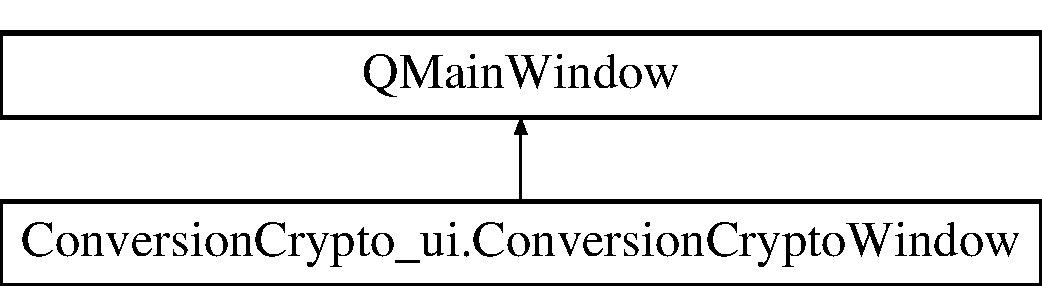
\includegraphics[height=2.000000cm]{class_conversion_crypto__ui_1_1_conversion_crypto_window}
\end{center}
\end{figure}
\subsection*{Public Member Functions}
\begin{DoxyCompactItemize}
\item 
def \hyperlink{class_conversion_crypto__ui_1_1_conversion_crypto_window_a2c076dd5a4c7905c9e8898ace06516ad}{\+\_\+\+\_\+init\+\_\+\+\_\+} (self, path=\char`\"{}\char`\"{})
\begin{DoxyCompactList}\small\item\em The constructor of the crypto conversion window. \end{DoxyCompactList}\item 
def \hyperlink{class_conversion_crypto__ui_1_1_conversion_crypto_window_a1348e819d5c05e07ccf156235ba333e9}{cryptoconvert} (self)
\begin{DoxyCompactList}\small\item\em Displays the conversion a value of a base type 1 to a value of base type 2. \end{DoxyCompactList}\item 
\mbox{\Hypertarget{class_conversion_crypto__ui_1_1_conversion_crypto_window_acde9f773c8b7d602583783e5eff85760}\label{class_conversion_crypto__ui_1_1_conversion_crypto_window_acde9f773c8b7d602583783e5eff85760}} 
def {\bfseries close\+Event} (self, event)
\item 
\mbox{\Hypertarget{class_conversion_crypto__ui_1_1_conversion_crypto_window_a5918c0af343a4ad48a6251533d8eb1cf}\label{class_conversion_crypto__ui_1_1_conversion_crypto_window_a5918c0af343a4ad48a6251533d8eb1cf}} 
def \hyperlink{class_conversion_crypto__ui_1_1_conversion_crypto_window_a5918c0af343a4ad48a6251533d8eb1cf}{clear\+Fields} (self)
\begin{DoxyCompactList}\small\item\em Clears all input and output fields. \end{DoxyCompactList}\end{DoxyCompactItemize}
\subsection*{Public Attributes}
\begin{DoxyCompactItemize}
\item 
\mbox{\Hypertarget{class_conversion_crypto__ui_1_1_conversion_crypto_window_af293f3d2991869ffc4859104d09dde98}\label{class_conversion_crypto__ui_1_1_conversion_crypto_window_af293f3d2991869ffc4859104d09dde98}} 
{\bfseries path}
\end{DoxyCompactItemize}


\subsection{Detailed Description}
\hyperlink{class_conversion_crypto__ui_1_1_conversion_crypto_window}{Conversion\+Crypto\+Window} is a class that implements the G\+UI components for the crypto conversion operation. 

\subsection{Constructor \& Destructor Documentation}
\mbox{\Hypertarget{class_conversion_crypto__ui_1_1_conversion_crypto_window_a2c076dd5a4c7905c9e8898ace06516ad}\label{class_conversion_crypto__ui_1_1_conversion_crypto_window_a2c076dd5a4c7905c9e8898ace06516ad}} 
\index{Conversion\+Crypto\+\_\+ui\+::\+Conversion\+Crypto\+Window@{Conversion\+Crypto\+\_\+ui\+::\+Conversion\+Crypto\+Window}!\+\_\+\+\_\+init\+\_\+\+\_\+@{\+\_\+\+\_\+init\+\_\+\+\_\+}}
\index{\+\_\+\+\_\+init\+\_\+\+\_\+@{\+\_\+\+\_\+init\+\_\+\+\_\+}!Conversion\+Crypto\+\_\+ui\+::\+Conversion\+Crypto\+Window@{Conversion\+Crypto\+\_\+ui\+::\+Conversion\+Crypto\+Window}}
\subsubsection{\texorpdfstring{\+\_\+\+\_\+init\+\_\+\+\_\+()}{\_\_init\_\_()}}
{\footnotesize\ttfamily def Conversion\+Crypto\+\_\+ui.\+Conversion\+Crypto\+Window.\+\_\+\+\_\+init\+\_\+\+\_\+ (\begin{DoxyParamCaption}\item[{}]{self,  }\item[{}]{path = {\ttfamily \char`\"{}\char`\"{}} }\end{DoxyParamCaption})}



The constructor of the crypto conversion window. 

Creates a pop up window that displays and sets up the buttons and input fields that are necessary to obtain input from the user and calculate the appropriate answer. Also sets up the window according to the created style sheet. 
\begin{DoxyParams}{Parameters}
{\em path} & The current path on which the file is found. Default value is an empty path. \\
\hline
\end{DoxyParams}


\subsection{Member Function Documentation}
\mbox{\Hypertarget{class_conversion_crypto__ui_1_1_conversion_crypto_window_a1348e819d5c05e07ccf156235ba333e9}\label{class_conversion_crypto__ui_1_1_conversion_crypto_window_a1348e819d5c05e07ccf156235ba333e9}} 
\index{Conversion\+Crypto\+\_\+ui\+::\+Conversion\+Crypto\+Window@{Conversion\+Crypto\+\_\+ui\+::\+Conversion\+Crypto\+Window}!cryptoconvert@{cryptoconvert}}
\index{cryptoconvert@{cryptoconvert}!Conversion\+Crypto\+\_\+ui\+::\+Conversion\+Crypto\+Window@{Conversion\+Crypto\+\_\+ui\+::\+Conversion\+Crypto\+Window}}
\subsubsection{\texorpdfstring{cryptoconvert()}{cryptoconvert()}}
{\footnotesize\ttfamily def Conversion\+Crypto\+\_\+ui.\+Conversion\+Crypto\+Window.\+cryptoconvert (\begin{DoxyParamCaption}\item[{}]{self }\end{DoxyParamCaption})}



Displays the conversion a value of a base type 1 to a value of base type 2. 

Takes in 1 value and the convert to and convert from type as input from the user through input fields and shows the user the result on the window 

The documentation for this class was generated from the following file\+:\begin{DoxyCompactItemize}
\item 
src/uis/\hyperlink{_conversion_crypto__ui_8py}{Conversion\+Crypto\+\_\+ui.\+py}\end{DoxyCompactItemize}

\hypertarget{class_conversion_currency__ui_1_1_conversion_currency_window}{}\section{Conversion\+Currency\+\_\+ui.\+Conversion\+Currency\+Window Class Reference}
\label{class_conversion_currency__ui_1_1_conversion_currency_window}\index{Conversion\+Currency\+\_\+ui.\+Conversion\+Currency\+Window@{Conversion\+Currency\+\_\+ui.\+Conversion\+Currency\+Window}}


Conversion\+Base\+Window is a class that implements the G\+UI components for the currency conversion operation.  


Inheritance diagram for Conversion\+Currency\+\_\+ui.\+Conversion\+Currency\+Window\+:\begin{figure}[H]
\begin{center}
\leavevmode
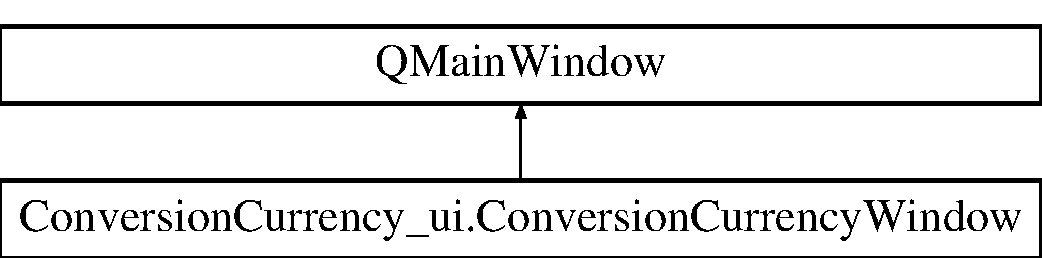
\includegraphics[height=2.000000cm]{class_conversion_currency__ui_1_1_conversion_currency_window}
\end{center}
\end{figure}
\subsection*{Public Member Functions}
\begin{DoxyCompactItemize}
\item 
def \hyperlink{class_conversion_currency__ui_1_1_conversion_currency_window_a5219de9caa768775d8a5c638bb20cd17}{\+\_\+\+\_\+init\+\_\+\+\_\+} (self, path=\char`\"{}\char`\"{})
\begin{DoxyCompactList}\small\item\em The constructor of the currency conversion window. \end{DoxyCompactList}\item 
def \hyperlink{class_conversion_currency__ui_1_1_conversion_currency_window_ad8504b8dbbe0d321f4c2374e17c92fcf}{currconvert} (self)
\begin{DoxyCompactList}\small\item\em Displays the conversion a value of a base type 1 to a value of base type 2. \end{DoxyCompactList}\item 
\mbox{\Hypertarget{class_conversion_currency__ui_1_1_conversion_currency_window_a80345912920b77fcf8d91285cd60a6fd}\label{class_conversion_currency__ui_1_1_conversion_currency_window_a80345912920b77fcf8d91285cd60a6fd}} 
def {\bfseries close\+Event} (self, event)
\item 
\mbox{\Hypertarget{class_conversion_currency__ui_1_1_conversion_currency_window_a1f0d0ca2a89ced1a26380744dbdb73dc}\label{class_conversion_currency__ui_1_1_conversion_currency_window_a1f0d0ca2a89ced1a26380744dbdb73dc}} 
def \hyperlink{class_conversion_currency__ui_1_1_conversion_currency_window_a1f0d0ca2a89ced1a26380744dbdb73dc}{clear\+Fields} (self)
\begin{DoxyCompactList}\small\item\em Clears all input and output fields. \end{DoxyCompactList}\end{DoxyCompactItemize}
\subsection*{Public Attributes}
\begin{DoxyCompactItemize}
\item 
\mbox{\Hypertarget{class_conversion_currency__ui_1_1_conversion_currency_window_af9c27d4f866095863b98223f4687dfae}\label{class_conversion_currency__ui_1_1_conversion_currency_window_af9c27d4f866095863b98223f4687dfae}} 
{\bfseries path}
\end{DoxyCompactItemize}


\subsection{Detailed Description}
Conversion\+Base\+Window is a class that implements the G\+UI components for the currency conversion operation. 

\subsection{Constructor \& Destructor Documentation}
\mbox{\Hypertarget{class_conversion_currency__ui_1_1_conversion_currency_window_a5219de9caa768775d8a5c638bb20cd17}\label{class_conversion_currency__ui_1_1_conversion_currency_window_a5219de9caa768775d8a5c638bb20cd17}} 
\index{Conversion\+Currency\+\_\+ui\+::\+Conversion\+Currency\+Window@{Conversion\+Currency\+\_\+ui\+::\+Conversion\+Currency\+Window}!\+\_\+\+\_\+init\+\_\+\+\_\+@{\+\_\+\+\_\+init\+\_\+\+\_\+}}
\index{\+\_\+\+\_\+init\+\_\+\+\_\+@{\+\_\+\+\_\+init\+\_\+\+\_\+}!Conversion\+Currency\+\_\+ui\+::\+Conversion\+Currency\+Window@{Conversion\+Currency\+\_\+ui\+::\+Conversion\+Currency\+Window}}
\subsubsection{\texorpdfstring{\+\_\+\+\_\+init\+\_\+\+\_\+()}{\_\_init\_\_()}}
{\footnotesize\ttfamily def Conversion\+Currency\+\_\+ui.\+Conversion\+Currency\+Window.\+\_\+\+\_\+init\+\_\+\+\_\+ (\begin{DoxyParamCaption}\item[{}]{self,  }\item[{}]{path = {\ttfamily \char`\"{}\char`\"{}} }\end{DoxyParamCaption})}



The constructor of the currency conversion window. 

Creates a pop up window that displays and sets up the buttons and input fields that are necessary to obtain input from the user and calculate the appropriate answer. Also sets up the window according to the created style sheet. 
\begin{DoxyParams}{Parameters}
{\em path} & The current path on which the file is found. Default value is an empty path. \\
\hline
\end{DoxyParams}


\subsection{Member Function Documentation}
\mbox{\Hypertarget{class_conversion_currency__ui_1_1_conversion_currency_window_ad8504b8dbbe0d321f4c2374e17c92fcf}\label{class_conversion_currency__ui_1_1_conversion_currency_window_ad8504b8dbbe0d321f4c2374e17c92fcf}} 
\index{Conversion\+Currency\+\_\+ui\+::\+Conversion\+Currency\+Window@{Conversion\+Currency\+\_\+ui\+::\+Conversion\+Currency\+Window}!currconvert@{currconvert}}
\index{currconvert@{currconvert}!Conversion\+Currency\+\_\+ui\+::\+Conversion\+Currency\+Window@{Conversion\+Currency\+\_\+ui\+::\+Conversion\+Currency\+Window}}
\subsubsection{\texorpdfstring{currconvert()}{currconvert()}}
{\footnotesize\ttfamily def Conversion\+Currency\+\_\+ui.\+Conversion\+Currency\+Window.\+currconvert (\begin{DoxyParamCaption}\item[{}]{self }\end{DoxyParamCaption})}



Displays the conversion a value of a base type 1 to a value of base type 2. 

Takes in 1 value and the convert to and convert from type as input from the user through input fields and shows the user the result on the window 

The documentation for this class was generated from the following file\+:\begin{DoxyCompactItemize}
\item 
src/uis/\hyperlink{_conversion_currency__ui_8py}{Conversion\+Currency\+\_\+ui.\+py}\end{DoxyCompactItemize}

\hypertarget{class_conversion_r_n__ui_1_1_conversion_r_n_window}{}\section{Conversion\+R\+N\+\_\+ui.\+Conversion\+R\+N\+Window Class Reference}
\label{class_conversion_r_n__ui_1_1_conversion_r_n_window}\index{Conversion\+R\+N\+\_\+ui.\+Conversion\+R\+N\+Window@{Conversion\+R\+N\+\_\+ui.\+Conversion\+R\+N\+Window}}


Conversion\+Base\+Window is a class that implements the G\+UI components for the roman numeral conversion operation.  


Inheritance diagram for Conversion\+R\+N\+\_\+ui.\+Conversion\+R\+N\+Window\+:\begin{figure}[H]
\begin{center}
\leavevmode
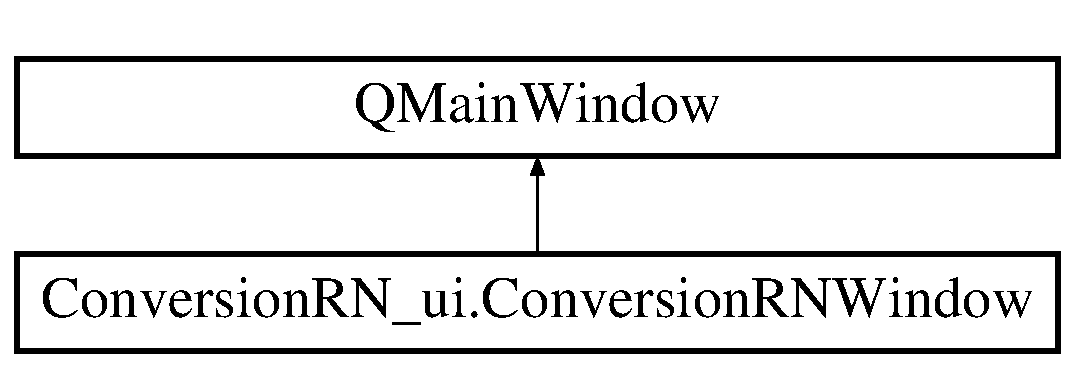
\includegraphics[height=2.000000cm]{class_conversion_r_n__ui_1_1_conversion_r_n_window}
\end{center}
\end{figure}
\subsection*{Public Member Functions}
\begin{DoxyCompactItemize}
\item 
def \hyperlink{class_conversion_r_n__ui_1_1_conversion_r_n_window_aa4752dfe8364faa4649c2c19ff55fba6}{\+\_\+\+\_\+init\+\_\+\+\_\+} (self, path=\char`\"{}\char`\"{})
\begin{DoxyCompactList}\small\item\em The constructor of the roman numeral conversion window. \end{DoxyCompactList}\item 
def \hyperlink{class_conversion_r_n__ui_1_1_conversion_r_n_window_a0c015e92809a27ecde70f4b62e102da4}{R\+Nconvert} (self)
\begin{DoxyCompactList}\small\item\em Displays the conversion a value of a base type 1 to a value of base type 2. \end{DoxyCompactList}\end{DoxyCompactItemize}
\subsection*{Public Attributes}
\begin{DoxyCompactItemize}
\item 
\mbox{\Hypertarget{class_conversion_r_n__ui_1_1_conversion_r_n_window_aa7468d2c903a7f327f268ac030509639}\label{class_conversion_r_n__ui_1_1_conversion_r_n_window_aa7468d2c903a7f327f268ac030509639}} 
{\bfseries path}
\end{DoxyCompactItemize}


\subsection{Detailed Description}
Conversion\+Base\+Window is a class that implements the G\+UI components for the roman numeral conversion operation. 

\subsection{Constructor \& Destructor Documentation}
\mbox{\Hypertarget{class_conversion_r_n__ui_1_1_conversion_r_n_window_aa4752dfe8364faa4649c2c19ff55fba6}\label{class_conversion_r_n__ui_1_1_conversion_r_n_window_aa4752dfe8364faa4649c2c19ff55fba6}} 
\index{Conversion\+R\+N\+\_\+ui\+::\+Conversion\+R\+N\+Window@{Conversion\+R\+N\+\_\+ui\+::\+Conversion\+R\+N\+Window}!\+\_\+\+\_\+init\+\_\+\+\_\+@{\+\_\+\+\_\+init\+\_\+\+\_\+}}
\index{\+\_\+\+\_\+init\+\_\+\+\_\+@{\+\_\+\+\_\+init\+\_\+\+\_\+}!Conversion\+R\+N\+\_\+ui\+::\+Conversion\+R\+N\+Window@{Conversion\+R\+N\+\_\+ui\+::\+Conversion\+R\+N\+Window}}
\subsubsection{\texorpdfstring{\+\_\+\+\_\+init\+\_\+\+\_\+()}{\_\_init\_\_()}}
{\footnotesize\ttfamily def Conversion\+R\+N\+\_\+ui.\+Conversion\+R\+N\+Window.\+\_\+\+\_\+init\+\_\+\+\_\+ (\begin{DoxyParamCaption}\item[{}]{self,  }\item[{}]{path = {\ttfamily \char`\"{}\char`\"{}} }\end{DoxyParamCaption})}



The constructor of the roman numeral conversion window. 

Creates a pop up window that displays and sets up the buttons and input fields that are necessary to obtain input from the user and calculate the appropriate answer. Also sets up the window according to the created style sheet. 
\begin{DoxyParams}{Parameters}
{\em path} & The current path on which the file is found. Default value is an empty path. \\
\hline
\end{DoxyParams}


\subsection{Member Function Documentation}
\mbox{\Hypertarget{class_conversion_r_n__ui_1_1_conversion_r_n_window_a0c015e92809a27ecde70f4b62e102da4}\label{class_conversion_r_n__ui_1_1_conversion_r_n_window_a0c015e92809a27ecde70f4b62e102da4}} 
\index{Conversion\+R\+N\+\_\+ui\+::\+Conversion\+R\+N\+Window@{Conversion\+R\+N\+\_\+ui\+::\+Conversion\+R\+N\+Window}!R\+Nconvert@{R\+Nconvert}}
\index{R\+Nconvert@{R\+Nconvert}!Conversion\+R\+N\+\_\+ui\+::\+Conversion\+R\+N\+Window@{Conversion\+R\+N\+\_\+ui\+::\+Conversion\+R\+N\+Window}}
\subsubsection{\texorpdfstring{R\+Nconvert()}{RNconvert()}}
{\footnotesize\ttfamily def Conversion\+R\+N\+\_\+ui.\+Conversion\+R\+N\+Window.\+R\+Nconvert (\begin{DoxyParamCaption}\item[{}]{self }\end{DoxyParamCaption})}



Displays the conversion a value of a base type 1 to a value of base type 2. 

Takes in 1 value and the convert to and convert from type as input from the user through input fields and shows the user the result on the window 

The documentation for this class was generated from the following file\+:\begin{DoxyCompactItemize}
\item 
src/uis/\hyperlink{_conversion_r_n__ui_8py}{Conversion\+R\+N\+\_\+ui.\+py}\end{DoxyCompactItemize}

\hypertarget{class_conversion__ui_1_1_converter_window}{}\section{Conversion\+\_\+ui.\+Converter\+Window Class Reference}
\label{class_conversion__ui_1_1_converter_window}\index{Conversion\+\_\+ui.\+Converter\+Window@{Conversion\+\_\+ui.\+Converter\+Window}}


\hyperlink{class_conversion__ui_1_1_converter_window}{Converter\+Window} is a class that implements the G\+UI components for the Conversion operation menu.  


Inheritance diagram for Conversion\+\_\+ui.\+Converter\+Window\+:\begin{figure}[H]
\begin{center}
\leavevmode
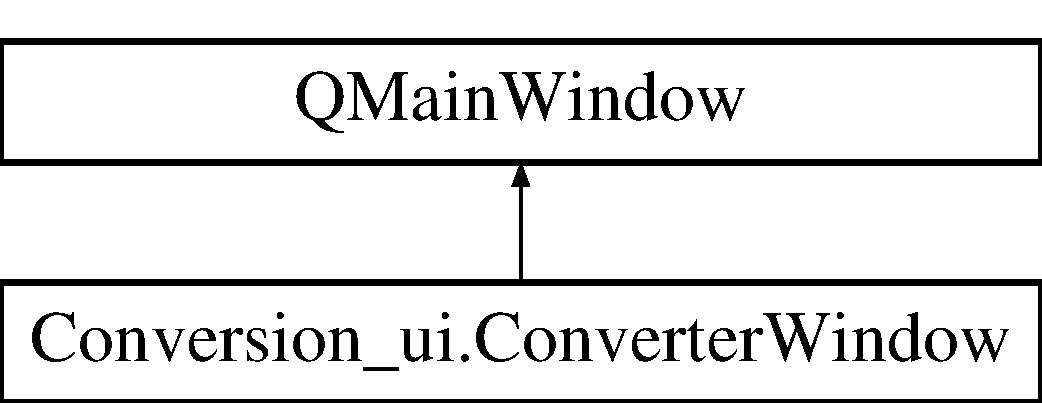
\includegraphics[height=2.000000cm]{class_conversion__ui_1_1_converter_window}
\end{center}
\end{figure}
\subsection*{Public Member Functions}
\begin{DoxyCompactItemize}
\item 
def \hyperlink{class_conversion__ui_1_1_converter_window_a3ae25e516ec55570394c9a171301dd02}{\+\_\+\+\_\+init\+\_\+\+\_\+} (self, path=\char`\"{}\char`\"{})
\begin{DoxyCompactList}\small\item\em The constructor of the Conversion window. \end{DoxyCompactList}\end{DoxyCompactItemize}
\subsection*{Public Attributes}
\begin{DoxyCompactItemize}
\item 
\mbox{\Hypertarget{class_conversion__ui_1_1_converter_window_a5ec5f7f6dfc309b53d3913aa68c19d62}\label{class_conversion__ui_1_1_converter_window_a5ec5f7f6dfc309b53d3913aa68c19d62}} 
{\bfseries path}
\item 
\mbox{\Hypertarget{class_conversion__ui_1_1_converter_window_a5857c0c4c106f6b4a9e4f432f7bba334}\label{class_conversion__ui_1_1_converter_window_a5857c0c4c106f6b4a9e4f432f7bba334}} 
{\bfseries xpath}
\item 
\mbox{\Hypertarget{class_conversion__ui_1_1_converter_window_a325e2ca2e9f7b127aab5db5fba91cc0c}\label{class_conversion__ui_1_1_converter_window_a325e2ca2e9f7b127aab5db5fba91cc0c}} 
{\bfseries currency}
\item 
\mbox{\Hypertarget{class_conversion__ui_1_1_converter_window_ad3285dceff06a5baa0da5e15de409019}\label{class_conversion__ui_1_1_converter_window_ad3285dceff06a5baa0da5e15de409019}} 
{\bfseries base}
\item 
\mbox{\Hypertarget{class_conversion__ui_1_1_converter_window_ae8518028eb09118845ff07b6f0c61ac1}\label{class_conversion__ui_1_1_converter_window_ae8518028eb09118845ff07b6f0c61ac1}} 
{\bfseries crypto}
\item 
\mbox{\Hypertarget{class_conversion__ui_1_1_converter_window_abc4821c75d272db17d4c5adade36e359}\label{class_conversion__ui_1_1_converter_window_abc4821c75d272db17d4c5adade36e359}} 
{\bfseries RN}
\end{DoxyCompactItemize}


\subsection{Detailed Description}
\hyperlink{class_conversion__ui_1_1_converter_window}{Converter\+Window} is a class that implements the G\+UI components for the Conversion operation menu. 

\subsection{Constructor \& Destructor Documentation}
\mbox{\Hypertarget{class_conversion__ui_1_1_converter_window_a3ae25e516ec55570394c9a171301dd02}\label{class_conversion__ui_1_1_converter_window_a3ae25e516ec55570394c9a171301dd02}} 
\index{Conversion\+\_\+ui\+::\+Converter\+Window@{Conversion\+\_\+ui\+::\+Converter\+Window}!\+\_\+\+\_\+init\+\_\+\+\_\+@{\+\_\+\+\_\+init\+\_\+\+\_\+}}
\index{\+\_\+\+\_\+init\+\_\+\+\_\+@{\+\_\+\+\_\+init\+\_\+\+\_\+}!Conversion\+\_\+ui\+::\+Converter\+Window@{Conversion\+\_\+ui\+::\+Converter\+Window}}
\subsubsection{\texorpdfstring{\+\_\+\+\_\+init\+\_\+\+\_\+()}{\_\_init\_\_()}}
{\footnotesize\ttfamily def Conversion\+\_\+ui.\+Converter\+Window.\+\_\+\+\_\+init\+\_\+\+\_\+ (\begin{DoxyParamCaption}\item[{}]{self,  }\item[{}]{path = {\ttfamily \char`\"{}\char`\"{}} }\end{DoxyParamCaption})}



The constructor of the Conversion window. 

Creates a pop up window that displays and sets up the buttons that are necessary to navigate from the Conversion window to other parts of the application. Also sets up the Conversion window according to the created style sheet. 
\begin{DoxyParams}{Parameters}
{\em path} & The current path on which the file is found. Default value is an empty path. \\
\hline
\end{DoxyParams}


The documentation for this class was generated from the following file\+:\begin{DoxyCompactItemize}
\item 
src/uis/\hyperlink{_conversion__ui_8py}{Conversion\+\_\+ui.\+py}\end{DoxyCompactItemize}

\hypertarget{classfloating__point__ui_1_1_floating_point_window}{}\section{floating\+\_\+point\+\_\+ui.\+Floating\+Point\+Window Class Reference}
\label{classfloating__point__ui_1_1_floating_point_window}\index{floating\+\_\+point\+\_\+ui.\+Floating\+Point\+Window@{floating\+\_\+point\+\_\+ui.\+Floating\+Point\+Window}}


\hyperlink{classfloating__point__ui_1_1_floating_point_window}{Floating\+Point\+Window} is a class that implements the G\+UI components for the Floating Point operation.  


Inheritance diagram for floating\+\_\+point\+\_\+ui.\+Floating\+Point\+Window\+:\begin{figure}[H]
\begin{center}
\leavevmode
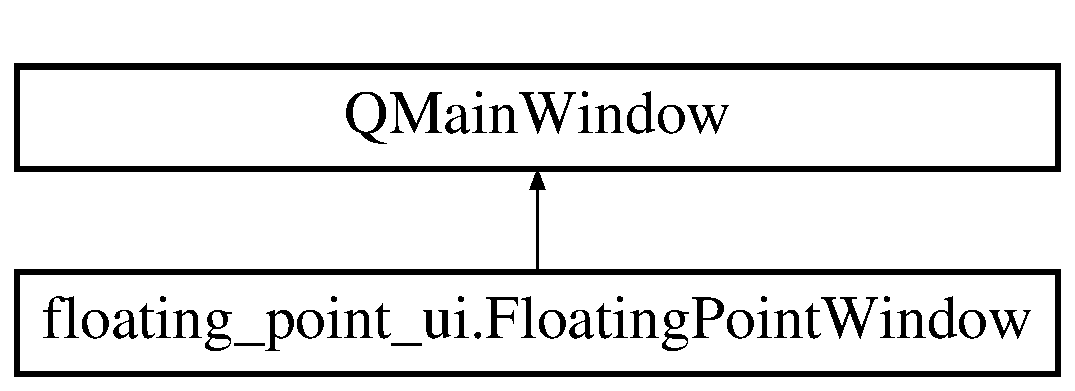
\includegraphics[height=2.000000cm]{classfloating__point__ui_1_1_floating_point_window}
\end{center}
\end{figure}
\subsection*{Public Member Functions}
\begin{DoxyCompactItemize}
\item 
def \hyperlink{classfloating__point__ui_1_1_floating_point_window_ab5a1e532591e07c6ad7603c561532979}{\+\_\+\+\_\+init\+\_\+\+\_\+} (self, path=\char`\"{}\char`\"{})
\begin{DoxyCompactList}\small\item\em The constructor of the Floating Point window. \end{DoxyCompactList}\item 
def \hyperlink{classfloating__point__ui_1_1_floating_point_window_a3e36de9fde9b6387740d13a644fdfc56}{floating\+\_\+point} (self)
\begin{DoxyCompactList}\small\item\em Displays the conversion of a decimal number to I\+E\+EE 754 floating point representation and vice versa. \end{DoxyCompactList}\item 
\mbox{\Hypertarget{classfloating__point__ui_1_1_floating_point_window_aa84d9d4ad3c6fca9062c7b49c6d9e37e}\label{classfloating__point__ui_1_1_floating_point_window_aa84d9d4ad3c6fca9062c7b49c6d9e37e}} 
def \hyperlink{classfloating__point__ui_1_1_floating_point_window_aa84d9d4ad3c6fca9062c7b49c6d9e37e}{close\+Event} (self, event)
\begin{DoxyCompactList}\small\item\em Closes window and clears inputs upon close. \end{DoxyCompactList}\item 
\mbox{\Hypertarget{classfloating__point__ui_1_1_floating_point_window_aff0f79ab51ec2f1a373780b37848d700}\label{classfloating__point__ui_1_1_floating_point_window_aff0f79ab51ec2f1a373780b37848d700}} 
def \hyperlink{classfloating__point__ui_1_1_floating_point_window_aff0f79ab51ec2f1a373780b37848d700}{clear\+Fields} (self)
\begin{DoxyCompactList}\small\item\em Clears all input and output fields. \end{DoxyCompactList}\end{DoxyCompactItemize}
\subsection*{Public Attributes}
\begin{DoxyCompactItemize}
\item 
\mbox{\Hypertarget{classfloating__point__ui_1_1_floating_point_window_aa40210a7ef669d041d3f4ea1880a4047}\label{classfloating__point__ui_1_1_floating_point_window_aa40210a7ef669d041d3f4ea1880a4047}} 
{\bfseries path}
\end{DoxyCompactItemize}


\subsection{Detailed Description}
\hyperlink{classfloating__point__ui_1_1_floating_point_window}{Floating\+Point\+Window} is a class that implements the G\+UI components for the Floating Point operation. 

\subsection{Constructor \& Destructor Documentation}
\mbox{\Hypertarget{classfloating__point__ui_1_1_floating_point_window_ab5a1e532591e07c6ad7603c561532979}\label{classfloating__point__ui_1_1_floating_point_window_ab5a1e532591e07c6ad7603c561532979}} 
\index{floating\+\_\+point\+\_\+ui\+::\+Floating\+Point\+Window@{floating\+\_\+point\+\_\+ui\+::\+Floating\+Point\+Window}!\+\_\+\+\_\+init\+\_\+\+\_\+@{\+\_\+\+\_\+init\+\_\+\+\_\+}}
\index{\+\_\+\+\_\+init\+\_\+\+\_\+@{\+\_\+\+\_\+init\+\_\+\+\_\+}!floating\+\_\+point\+\_\+ui\+::\+Floating\+Point\+Window@{floating\+\_\+point\+\_\+ui\+::\+Floating\+Point\+Window}}
\subsubsection{\texorpdfstring{\+\_\+\+\_\+init\+\_\+\+\_\+()}{\_\_init\_\_()}}
{\footnotesize\ttfamily def floating\+\_\+point\+\_\+ui.\+Floating\+Point\+Window.\+\_\+\+\_\+init\+\_\+\+\_\+ (\begin{DoxyParamCaption}\item[{}]{self,  }\item[{}]{path = {\ttfamily \char`\"{}\char`\"{}} }\end{DoxyParamCaption})}



The constructor of the Floating Point window. 

Creates a pop up window that displays and sets up the buttons and input fields that are necessary to obtain input from the user and calculate the appropriate answer. Also sets up the window according to the created style sheet. 
\begin{DoxyParams}{Parameters}
{\em path} & The current path on which the file is found. Default value is an empty path. \\
\hline
\end{DoxyParams}


\subsection{Member Function Documentation}
\mbox{\Hypertarget{classfloating__point__ui_1_1_floating_point_window_a3e36de9fde9b6387740d13a644fdfc56}\label{classfloating__point__ui_1_1_floating_point_window_a3e36de9fde9b6387740d13a644fdfc56}} 
\index{floating\+\_\+point\+\_\+ui\+::\+Floating\+Point\+Window@{floating\+\_\+point\+\_\+ui\+::\+Floating\+Point\+Window}!floating\+\_\+point@{floating\+\_\+point}}
\index{floating\+\_\+point@{floating\+\_\+point}!floating\+\_\+point\+\_\+ui\+::\+Floating\+Point\+Window@{floating\+\_\+point\+\_\+ui\+::\+Floating\+Point\+Window}}
\subsubsection{\texorpdfstring{floating\+\_\+point()}{floating\_point()}}
{\footnotesize\ttfamily def floating\+\_\+point\+\_\+ui.\+Floating\+Point\+Window.\+floating\+\_\+point (\begin{DoxyParamCaption}\item[{}]{self }\end{DoxyParamCaption})}



Displays the conversion of a decimal number to I\+E\+EE 754 floating point representation and vice versa. 

Takes in decimal number or floating point number from the user through input fields, and shows the user the result on the window 

The documentation for this class was generated from the following file\+:\begin{DoxyCompactItemize}
\item 
src/uis/\hyperlink{floating__point__ui_8py}{floating\+\_\+point\+\_\+ui.\+py}\end{DoxyCompactItemize}

\hypertarget{classgeometry__ui_1_1_geometry_window}{}\section{geometry\+\_\+ui.\+Geometry\+Window Class Reference}
\label{classgeometry__ui_1_1_geometry_window}\index{geometry\+\_\+ui.\+Geometry\+Window@{geometry\+\_\+ui.\+Geometry\+Window}}


\hyperlink{classgeometry__ui_1_1_geometry_window}{Geometry\+Window} is a class that implements the G\+UI components for the Geometry operation menu.  


Inheritance diagram for geometry\+\_\+ui.\+Geometry\+Window\+:\begin{figure}[H]
\begin{center}
\leavevmode
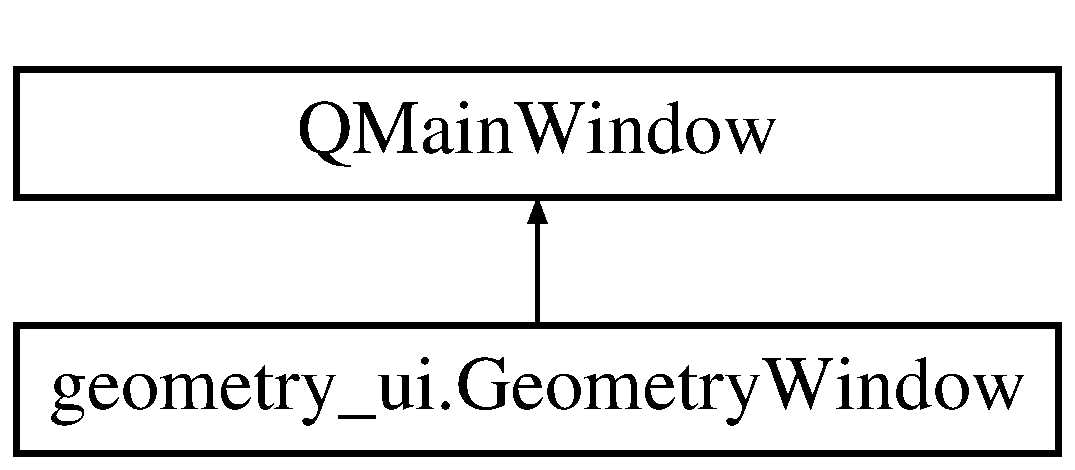
\includegraphics[height=2.000000cm]{classgeometry__ui_1_1_geometry_window}
\end{center}
\end{figure}
\subsection*{Public Member Functions}
\begin{DoxyCompactItemize}
\item 
def \hyperlink{classgeometry__ui_1_1_geometry_window_af619e3ecabaa9592f6de5987e31a27d3}{\+\_\+\+\_\+init\+\_\+\+\_\+} (self, path=\char`\"{}\char`\"{})
\begin{DoxyCompactList}\small\item\em The constructor of the Geometry window. \end{DoxyCompactList}\item 
\mbox{\Hypertarget{classgeometry__ui_1_1_geometry_window_a0374b136f1af38239cee73a36f500cbf}\label{classgeometry__ui_1_1_geometry_window_a0374b136f1af38239cee73a36f500cbf}} 
def \hyperlink{classgeometry__ui_1_1_geometry_window_a0374b136f1af38239cee73a36f500cbf}{close\+Event} (self, event)
\begin{DoxyCompactList}\small\item\em Closes the window and any other geometry operation windows. \end{DoxyCompactList}\end{DoxyCompactItemize}
\subsection*{Public Attributes}
\begin{DoxyCompactItemize}
\item 
\mbox{\Hypertarget{classgeometry__ui_1_1_geometry_window_a8babe312d482e206b2dc7250ce38badf}\label{classgeometry__ui_1_1_geometry_window_a8babe312d482e206b2dc7250ce38badf}} 
{\bfseries path}
\item 
\mbox{\Hypertarget{classgeometry__ui_1_1_geometry_window_a152d50bcffbc41d48e48e5f4bc2a0b61}\label{classgeometry__ui_1_1_geometry_window_a152d50bcffbc41d48e48e5f4bc2a0b61}} 
{\bfseries xpath}
\item 
\mbox{\Hypertarget{classgeometry__ui_1_1_geometry_window_abe95fb2e2e9934f76bf9c22f5b95f057}\label{classgeometry__ui_1_1_geometry_window_abe95fb2e2e9934f76bf9c22f5b95f057}} 
{\bfseries a}
\item 
\mbox{\Hypertarget{classgeometry__ui_1_1_geometry_window_a83ef83274a5147d430b345e3e165da24}\label{classgeometry__ui_1_1_geometry_window_a83ef83274a5147d430b345e3e165da24}} 
{\bfseries p}
\item 
\mbox{\Hypertarget{classgeometry__ui_1_1_geometry_window_a6cf11c20a79daeba227001599c5e841f}\label{classgeometry__ui_1_1_geometry_window_a6cf11c20a79daeba227001599c5e841f}} 
{\bfseries v}
\end{DoxyCompactItemize}


\subsection{Detailed Description}
\hyperlink{classgeometry__ui_1_1_geometry_window}{Geometry\+Window} is a class that implements the G\+UI components for the Geometry operation menu. 

\subsection{Constructor \& Destructor Documentation}
\mbox{\Hypertarget{classgeometry__ui_1_1_geometry_window_af619e3ecabaa9592f6de5987e31a27d3}\label{classgeometry__ui_1_1_geometry_window_af619e3ecabaa9592f6de5987e31a27d3}} 
\index{geometry\+\_\+ui\+::\+Geometry\+Window@{geometry\+\_\+ui\+::\+Geometry\+Window}!\+\_\+\+\_\+init\+\_\+\+\_\+@{\+\_\+\+\_\+init\+\_\+\+\_\+}}
\index{\+\_\+\+\_\+init\+\_\+\+\_\+@{\+\_\+\+\_\+init\+\_\+\+\_\+}!geometry\+\_\+ui\+::\+Geometry\+Window@{geometry\+\_\+ui\+::\+Geometry\+Window}}
\subsubsection{\texorpdfstring{\+\_\+\+\_\+init\+\_\+\+\_\+()}{\_\_init\_\_()}}
{\footnotesize\ttfamily def geometry\+\_\+ui.\+Geometry\+Window.\+\_\+\+\_\+init\+\_\+\+\_\+ (\begin{DoxyParamCaption}\item[{}]{self,  }\item[{}]{path = {\ttfamily \char`\"{}\char`\"{}} }\end{DoxyParamCaption})}



The constructor of the Geometry window. 

Creates a pop up window that displays and sets up the buttons that are necessary to navigate from the Geometry window to other parts of the application. Also sets up the Geometry window according to the created style sheet. 
\begin{DoxyParams}{Parameters}
{\em path} & The current path on which the file is found. Default value is an empty path. \\
\hline
\end{DoxyParams}


The documentation for this class was generated from the following file\+:\begin{DoxyCompactItemize}
\item 
src/uis/\hyperlink{geometry__ui_8py}{geometry\+\_\+ui.\+py}\end{DoxyCompactItemize}

\hypertarget{classgpa__ui_1_1_g_p_a_window}{}\section{gpa\+\_\+ui.\+G\+P\+A\+Window Class Reference}
\label{classgpa__ui_1_1_g_p_a_window}\index{gpa\+\_\+ui.\+G\+P\+A\+Window@{gpa\+\_\+ui.\+G\+P\+A\+Window}}


\hyperlink{classgpa__ui_1_1_g_p_a_window}{G\+P\+A\+Window} is a class that implements the G\+UI components for the G\+PA operation menu.  


Inheritance diagram for gpa\+\_\+ui.\+G\+P\+A\+Window\+:\begin{figure}[H]
\begin{center}
\leavevmode
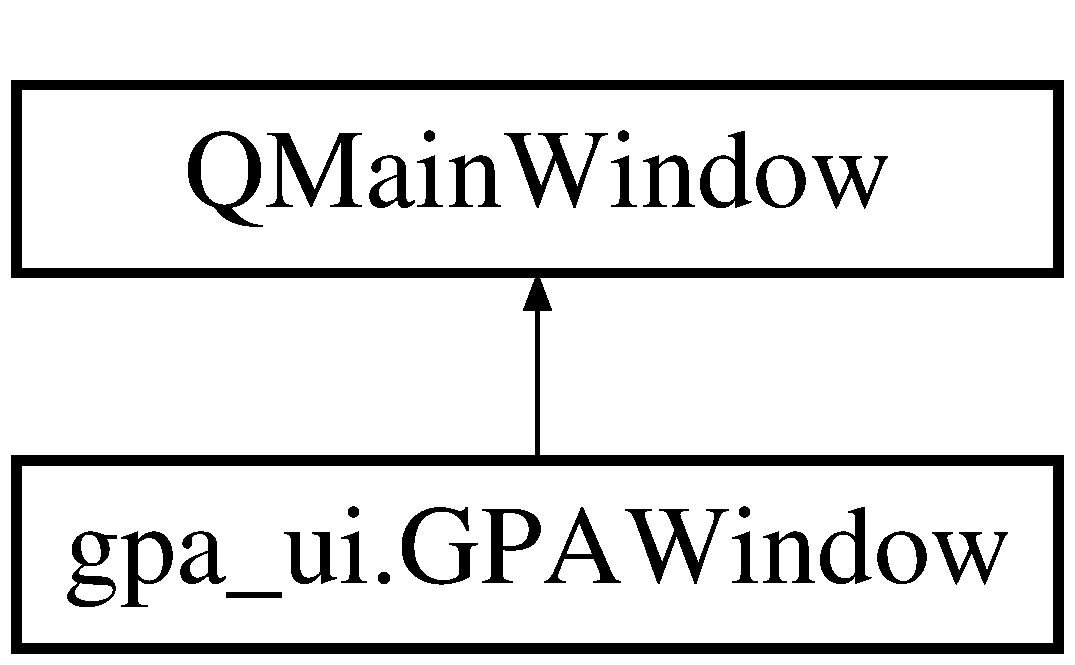
\includegraphics[height=2.000000cm]{classgpa__ui_1_1_g_p_a_window}
\end{center}
\end{figure}
\subsection*{Public Member Functions}
\begin{DoxyCompactItemize}
\item 
def \hyperlink{classgpa__ui_1_1_g_p_a_window_af341d6a11fb5030a5136cce247c95530}{\+\_\+\+\_\+init\+\_\+\+\_\+} (slef, path=\char`\"{}\char`\"{})
\begin{DoxyCompactList}\small\item\em The constructor of the G\+PA window. \end{DoxyCompactList}\item 
def \hyperlink{classgpa__ui_1_1_g_p_a_window_a36e992cfdee2fc99be76c95f6a342249}{gpa} (self)
\begin{DoxyCompactList}\small\item\em Displays the 12.\+0 gpa from the metrics the user provides. \end{DoxyCompactList}\end{DoxyCompactItemize}
\subsection*{Public Attributes}
\begin{DoxyCompactItemize}
\item 
\mbox{\Hypertarget{classgpa__ui_1_1_g_p_a_window_a34487c55a57218bbaac85f9d1d7ab75e}\label{classgpa__ui_1_1_g_p_a_window_a34487c55a57218bbaac85f9d1d7ab75e}} 
{\bfseries path}
\end{DoxyCompactItemize}


\subsection{Detailed Description}
\hyperlink{classgpa__ui_1_1_g_p_a_window}{G\+P\+A\+Window} is a class that implements the G\+UI components for the G\+PA operation menu. 

\subsection{Constructor \& Destructor Documentation}
\mbox{\Hypertarget{classgpa__ui_1_1_g_p_a_window_af341d6a11fb5030a5136cce247c95530}\label{classgpa__ui_1_1_g_p_a_window_af341d6a11fb5030a5136cce247c95530}} 
\index{gpa\+\_\+ui\+::\+G\+P\+A\+Window@{gpa\+\_\+ui\+::\+G\+P\+A\+Window}!\+\_\+\+\_\+init\+\_\+\+\_\+@{\+\_\+\+\_\+init\+\_\+\+\_\+}}
\index{\+\_\+\+\_\+init\+\_\+\+\_\+@{\+\_\+\+\_\+init\+\_\+\+\_\+}!gpa\+\_\+ui\+::\+G\+P\+A\+Window@{gpa\+\_\+ui\+::\+G\+P\+A\+Window}}
\subsubsection{\texorpdfstring{\+\_\+\+\_\+init\+\_\+\+\_\+()}{\_\_init\_\_()}}
{\footnotesize\ttfamily def gpa\+\_\+ui.\+G\+P\+A\+Window.\+\_\+\+\_\+init\+\_\+\+\_\+ (\begin{DoxyParamCaption}\item[{}]{slef,  }\item[{}]{path = {\ttfamily \char`\"{}\char`\"{}} }\end{DoxyParamCaption})}



The constructor of the G\+PA window. 

Creates a pop up window that displays and sets up the buttons that are necessary to navigate from the G\+PA window to other parts of the application. Also sets up the G\+PA window according to the created style sheet. 
\begin{DoxyParams}{Parameters}
{\em path} & The current path on which the file is found. Default value is an empty path. \\
\hline
\end{DoxyParams}


\subsection{Member Function Documentation}
\mbox{\Hypertarget{classgpa__ui_1_1_g_p_a_window_a36e992cfdee2fc99be76c95f6a342249}\label{classgpa__ui_1_1_g_p_a_window_a36e992cfdee2fc99be76c95f6a342249}} 
\index{gpa\+\_\+ui\+::\+G\+P\+A\+Window@{gpa\+\_\+ui\+::\+G\+P\+A\+Window}!gpa@{gpa}}
\index{gpa@{gpa}!gpa\+\_\+ui\+::\+G\+P\+A\+Window@{gpa\+\_\+ui\+::\+G\+P\+A\+Window}}
\subsubsection{\texorpdfstring{gpa()}{gpa()}}
{\footnotesize\ttfamily def gpa\+\_\+ui.\+G\+P\+A\+Window.\+gpa (\begin{DoxyParamCaption}\item[{}]{self }\end{DoxyParamCaption})}



Displays the 12.\+0 gpa from the metrics the user provides. 

Takes in the grades and their weights through input fields and shows the users G\+PA result on the window 

The documentation for this class was generated from the following file\+:\begin{DoxyCompactItemize}
\item 
src/uis/\hyperlink{gpa__ui_8py}{gpa\+\_\+ui.\+py}\end{DoxyCompactItemize}

\hypertarget{classhealth__ui_1_1_health_window}{}\section{health\+\_\+ui.\+Health\+Window Class Reference}
\label{classhealth__ui_1_1_health_window}\index{health\+\_\+ui.\+Health\+Window@{health\+\_\+ui.\+Health\+Window}}


\hyperlink{classhealth__ui_1_1_health_window}{Health\+Window} is a class that implements the G\+UI components for the Health operation menu.  


Inheritance diagram for health\+\_\+ui.\+Health\+Window\+:\begin{figure}[H]
\begin{center}
\leavevmode
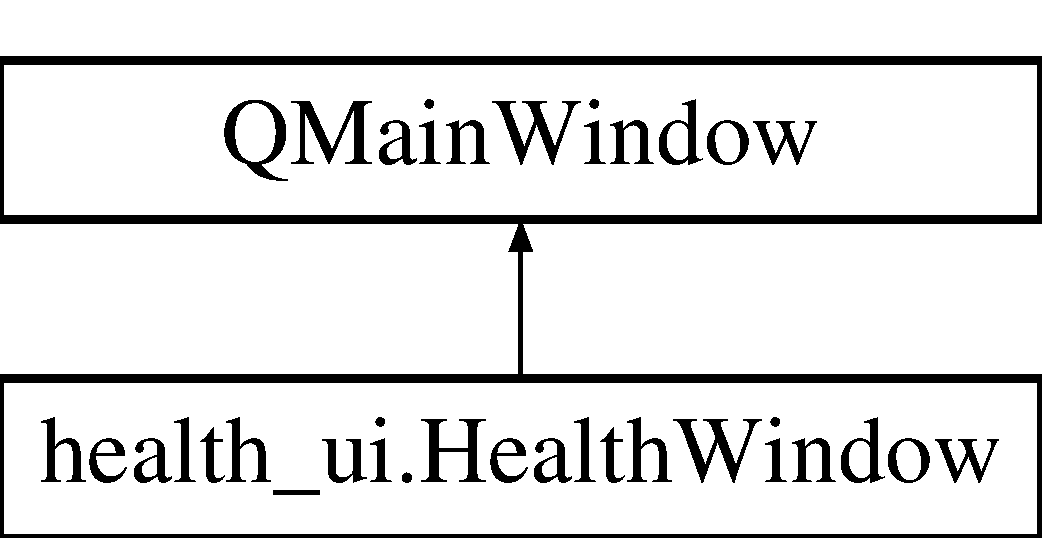
\includegraphics[height=2.000000cm]{classhealth__ui_1_1_health_window}
\end{center}
\end{figure}
\subsection*{Public Member Functions}
\begin{DoxyCompactItemize}
\item 
def \hyperlink{classhealth__ui_1_1_health_window_aca4eb93be30367445762dc27584bfde5}{\+\_\+\+\_\+init\+\_\+\+\_\+} (self, path=\char`\"{}\char`\"{})
\begin{DoxyCompactList}\small\item\em The constructor of the Health window. \end{DoxyCompactList}\item 
\mbox{\Hypertarget{classhealth__ui_1_1_health_window_a7b933fca8c05d872584f00a616dbd6de}\label{classhealth__ui_1_1_health_window_a7b933fca8c05d872584f00a616dbd6de}} 
def \hyperlink{classhealth__ui_1_1_health_window_a7b933fca8c05d872584f00a616dbd6de}{close\+Event} (self, event)
\begin{DoxyCompactList}\small\item\em Closes the window and any other health operation windows. \end{DoxyCompactList}\end{DoxyCompactItemize}
\subsection*{Public Attributes}
\begin{DoxyCompactItemize}
\item 
\mbox{\Hypertarget{classhealth__ui_1_1_health_window_a9b39fd0eb7f740de4266cfcc48110ff8}\label{classhealth__ui_1_1_health_window_a9b39fd0eb7f740de4266cfcc48110ff8}} 
{\bfseries path}
\item 
\mbox{\Hypertarget{classhealth__ui_1_1_health_window_a1bb4f7b081abe9c24b6b84b1c3bf3903}\label{classhealth__ui_1_1_health_window_a1bb4f7b081abe9c24b6b84b1c3bf3903}} 
{\bfseries xpath}
\item 
\mbox{\Hypertarget{classhealth__ui_1_1_health_window_ae3cbd4ee473d7a3f02023865dfcbd8c4}\label{classhealth__ui_1_1_health_window_ae3cbd4ee473d7a3f02023865dfcbd8c4}} 
{\bfseries bmi}
\item 
\mbox{\Hypertarget{classhealth__ui_1_1_health_window_a3e1494d47145602a31a0c0bb332690aa}\label{classhealth__ui_1_1_health_window_a3e1494d47145602a31a0c0bb332690aa}} 
{\bfseries bf}
\end{DoxyCompactItemize}


\subsection{Detailed Description}
\hyperlink{classhealth__ui_1_1_health_window}{Health\+Window} is a class that implements the G\+UI components for the Health operation menu. 

\subsection{Constructor \& Destructor Documentation}
\mbox{\Hypertarget{classhealth__ui_1_1_health_window_aca4eb93be30367445762dc27584bfde5}\label{classhealth__ui_1_1_health_window_aca4eb93be30367445762dc27584bfde5}} 
\index{health\+\_\+ui\+::\+Health\+Window@{health\+\_\+ui\+::\+Health\+Window}!\+\_\+\+\_\+init\+\_\+\+\_\+@{\+\_\+\+\_\+init\+\_\+\+\_\+}}
\index{\+\_\+\+\_\+init\+\_\+\+\_\+@{\+\_\+\+\_\+init\+\_\+\+\_\+}!health\+\_\+ui\+::\+Health\+Window@{health\+\_\+ui\+::\+Health\+Window}}
\subsubsection{\texorpdfstring{\+\_\+\+\_\+init\+\_\+\+\_\+()}{\_\_init\_\_()}}
{\footnotesize\ttfamily def health\+\_\+ui.\+Health\+Window.\+\_\+\+\_\+init\+\_\+\+\_\+ (\begin{DoxyParamCaption}\item[{}]{self,  }\item[{}]{path = {\ttfamily \char`\"{}\char`\"{}} }\end{DoxyParamCaption})}



The constructor of the Health window. 

Creates a pop up window that displays and sets up the buttons that are necessary to navigate from the Health window to other parts of the application. Also sets up the Health window according to the created style sheet. 
\begin{DoxyParams}{Parameters}
{\em path} & The current path on which the file is found. Default value is an empty path. \\
\hline
\end{DoxyParams}


The documentation for this class was generated from the following file\+:\begin{DoxyCompactItemize}
\item 
src/uis/\hyperlink{health__ui_8py}{health\+\_\+ui.\+py}\end{DoxyCompactItemize}

\hypertarget{classmain_1_1_main_window}{}\section{main.\+Main\+Window Class Reference}
\label{classmain_1_1_main_window}\index{main.\+Main\+Window@{main.\+Main\+Window}}


\hyperlink{classmain_1_1_main_window}{Main\+Window} is a class that implements the G\+UI components for the Main menu.  


Inheritance diagram for main.\+Main\+Window\+:\begin{figure}[H]
\begin{center}
\leavevmode
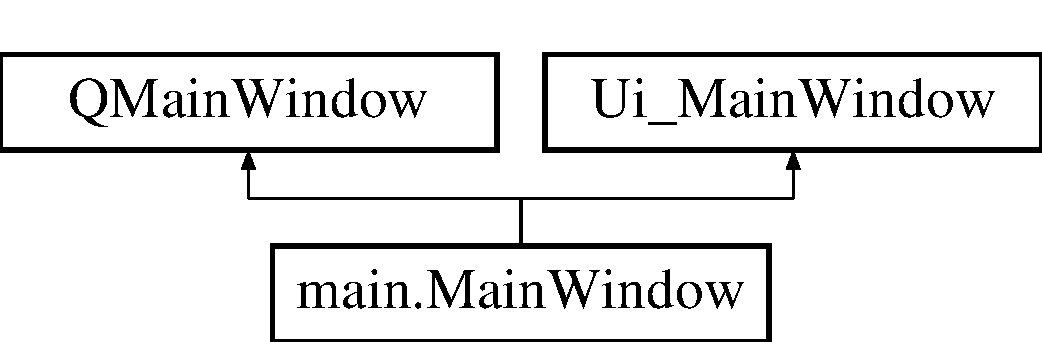
\includegraphics[height=2.000000cm]{classmain_1_1_main_window}
\end{center}
\end{figure}
\subsection*{Public Member Functions}
\begin{DoxyCompactItemize}
\item 
def \hyperlink{classmain_1_1_main_window_aafffd1d8e8955b1e04e531ad7f534b69}{\+\_\+\+\_\+init\+\_\+\+\_\+} (self, args, kwargs)
\begin{DoxyCompactList}\small\item\em The constructor of the Main window. \end{DoxyCompactList}\item 
def \hyperlink{classmain_1_1_main_window_a0888a2f2c8cd534806ea385502f1a67b}{store\+Mem} (self)
\begin{DoxyCompactList}\small\item\em Stores the current number. \end{DoxyCompactList}\item 
def \hyperlink{classmain_1_1_main_window_a77d526c3d373219cdd6d6d0437ac3660}{get\+Mem} (self)
\begin{DoxyCompactList}\small\item\em Displays current stored number. \end{DoxyCompactList}\item 
def \hyperlink{classmain_1_1_main_window_a86f6db688a227bf7a9228ef5ab650d31}{display} (self)
\begin{DoxyCompactList}\small\item\em Displays number to user. \end{DoxyCompactList}\item 
\mbox{\Hypertarget{classmain_1_1_main_window_aac70ce534fc78b51649a4692bce0db0d}\label{classmain_1_1_main_window_aac70ce534fc78b51649a4692bce0db0d}} 
def \hyperlink{classmain_1_1_main_window_aac70ce534fc78b51649a4692bce0db0d}{display\+Error} (self)
\begin{DoxyCompactList}\small\item\em Displays error message. \end{DoxyCompactList}\item 
def \hyperlink{classmain_1_1_main_window_a8d41e3c99603b99d23073aeea7d01534}{value\+Input} (self, v)
\begin{DoxyCompactList}\small\item\em Display value of input. \end{DoxyCompactList}\item 
def \hyperlink{classmain_1_1_main_window_a8e489d6d240a339dceb8258429fe1fc9}{reset} (self)
\begin{DoxyCompactList}\small\item\em Empty the line and current number stored. \end{DoxyCompactList}\item 
def \hyperlink{classmain_1_1_main_window_ad3673a13020c18149857ca57cbd13303}{addition} (self)
\begin{DoxyCompactList}\small\item\em Conducts calculator addition operation. \end{DoxyCompactList}\item 
def \hyperlink{classmain_1_1_main_window_a11dbd9c961cc33a4fe1bb87226810bca}{subtraction} (self)
\begin{DoxyCompactList}\small\item\em Conducts calculator subtraction operation. \end{DoxyCompactList}\item 
def \hyperlink{classmain_1_1_main_window_ac01c5ab4257a8aac093821c829ebbcd2}{multiplication} (self)
\begin{DoxyCompactList}\small\item\em Conducts calculator multiplication operation. \end{DoxyCompactList}\item 
def \hyperlink{classmain_1_1_main_window_a477f4d4d5bb5ef2805a250a36745ab4b}{power} (self)
\begin{DoxyCompactList}\small\item\em Conducts calculator power operation. \end{DoxyCompactList}\item 
def \hyperlink{classmain_1_1_main_window_a74162ce8832ff39d12773e129aaca8fb}{division} (self)
\begin{DoxyCompactList}\small\item\em Conducts calculator division operation. \end{DoxyCompactList}\item 
def \hyperlink{classmain_1_1_main_window_a2e0fc10335f0a466d3681cb2ca47d72c}{left\+\_\+bracket} (self)
\begin{DoxyCompactList}\small\item\em Adds left bracket operation. \end{DoxyCompactList}\item 
def \hyperlink{classmain_1_1_main_window_a5685744d7001c36a299b5e7ce984cf92}{right\+\_\+bracket} (self)
\begin{DoxyCompactList}\small\item\em Adds right bracket operation. \end{DoxyCompactList}\item 
def \hyperlink{classmain_1_1_main_window_a153d3cd5e2476e7f262d67600c77c1fc}{equals} (self)
\begin{DoxyCompactList}\small\item\em Evaluates operation. \end{DoxyCompactList}\item 
def \hyperlink{classmain_1_1_main_window_a298fe7db20162628212e8f665dc098f5}{key\+Press\+Event} (self, event)
\begin{DoxyCompactList}\small\item\em Runs functionality for each button click in the calculator. \end{DoxyCompactList}\item 
\mbox{\Hypertarget{classmain_1_1_main_window_a3c04a08e06ea9c36d998e3ee7ad99b30}\label{classmain_1_1_main_window_a3c04a08e06ea9c36d998e3ee7ad99b30}} 
def \hyperlink{classmain_1_1_main_window_a3c04a08e06ea9c36d998e3ee7ad99b30}{close\+Event} (self, event)
\begin{DoxyCompactList}\small\item\em Closes the window and any other open windows upon confirmation. \end{DoxyCompactList}\end{DoxyCompactItemize}
\subsection*{Static Public Member Functions}
\begin{DoxyCompactItemize}
\item 
\mbox{\Hypertarget{classmain_1_1_main_window_afbb14c9b37e09c14dff3f018c9a5d65a}\label{classmain_1_1_main_window_afbb14c9b37e09c14dff3f018c9a5d65a}} 
def {\bfseries credits} ()
\end{DoxyCompactItemize}
\subsection*{Public Attributes}
\begin{DoxyCompactItemize}
\item 
\mbox{\Hypertarget{classmain_1_1_main_window_ac90d4b9676d67b44447d3966a32d6417}\label{classmain_1_1_main_window_ac90d4b9676d67b44447d3966a32d6417}} 
{\bfseries converters}
\item 
\mbox{\Hypertarget{classmain_1_1_main_window_af9037d5b34cba2897b6f89da74e1a95b}\label{classmain_1_1_main_window_af9037d5b34cba2897b6f89da74e1a95b}} 
{\bfseries algebra}
\item 
\mbox{\Hypertarget{classmain_1_1_main_window_a584935749a42b7c6f5921beec9a5c100}\label{classmain_1_1_main_window_a584935749a42b7c6f5921beec9a5c100}} 
{\bfseries stock}
\item 
\mbox{\Hypertarget{classmain_1_1_main_window_aa6fae6477bf0cabf3e447cdb3a293511}\label{classmain_1_1_main_window_aa6fae6477bf0cabf3e447cdb3a293511}} 
{\bfseries health}
\item 
\mbox{\Hypertarget{classmain_1_1_main_window_a6da9e1bb50231a1bcb4ec434dfdc014a}\label{classmain_1_1_main_window_a6da9e1bb50231a1bcb4ec434dfdc014a}} 
{\bfseries gpa}
\item 
\mbox{\Hypertarget{classmain_1_1_main_window_abf63e5a9f6e37d9467383efacf218f01}\label{classmain_1_1_main_window_abf63e5a9f6e37d9467383efacf218f01}} 
{\bfseries binary}
\item 
\mbox{\Hypertarget{classmain_1_1_main_window_a838d54d37bed052ff6264f642d7527f7}\label{classmain_1_1_main_window_a838d54d37bed052ff6264f642d7527f7}} 
{\bfseries geo}
\item 
\mbox{\Hypertarget{classmain_1_1_main_window_aabad3594b4de0127995ff88be8e8f78f}\label{classmain_1_1_main_window_aabad3594b4de0127995ff88be8e8f78f}} 
{\bfseries calc}
\end{DoxyCompactItemize}


\subsection{Detailed Description}
\hyperlink{classmain_1_1_main_window}{Main\+Window} is a class that implements the G\+UI components for the Main menu. 

\subsection{Constructor \& Destructor Documentation}
\mbox{\Hypertarget{classmain_1_1_main_window_aafffd1d8e8955b1e04e531ad7f534b69}\label{classmain_1_1_main_window_aafffd1d8e8955b1e04e531ad7f534b69}} 
\index{main\+::\+Main\+Window@{main\+::\+Main\+Window}!\+\_\+\+\_\+init\+\_\+\+\_\+@{\+\_\+\+\_\+init\+\_\+\+\_\+}}
\index{\+\_\+\+\_\+init\+\_\+\+\_\+@{\+\_\+\+\_\+init\+\_\+\+\_\+}!main\+::\+Main\+Window@{main\+::\+Main\+Window}}
\subsubsection{\texorpdfstring{\+\_\+\+\_\+init\+\_\+\+\_\+()}{\_\_init\_\_()}}
{\footnotesize\ttfamily def main.\+Main\+Window.\+\_\+\+\_\+init\+\_\+\+\_\+ (\begin{DoxyParamCaption}\item[{}]{self,  }\item[{}]{args,  }\item[{}]{kwargs }\end{DoxyParamCaption})}



The constructor of the Main window. 

Creates a pop up window that displays and sets up the buttons that are necessary to navigate from the Main window to other parts of the application. Also sets up the Main window according to the created style sheet. 
\begin{DoxyParams}{Parameters}
{\em path} & The current path on which the file is found. Default value is an empty path. \\
\hline
\end{DoxyParams}


\subsection{Member Function Documentation}
\mbox{\Hypertarget{classmain_1_1_main_window_ad3673a13020c18149857ca57cbd13303}\label{classmain_1_1_main_window_ad3673a13020c18149857ca57cbd13303}} 
\index{main\+::\+Main\+Window@{main\+::\+Main\+Window}!addition@{addition}}
\index{addition@{addition}!main\+::\+Main\+Window@{main\+::\+Main\+Window}}
\subsubsection{\texorpdfstring{addition()}{addition()}}
{\footnotesize\ttfamily def main.\+Main\+Window.\+addition (\begin{DoxyParamCaption}\item[{}]{self }\end{DoxyParamCaption})}



Conducts calculator addition operation. 

Check if line input prior is not another operation and if it is not, display an empty string and adds an addition operation \mbox{\Hypertarget{classmain_1_1_main_window_a86f6db688a227bf7a9228ef5ab650d31}\label{classmain_1_1_main_window_a86f6db688a227bf7a9228ef5ab650d31}} 
\index{main\+::\+Main\+Window@{main\+::\+Main\+Window}!display@{display}}
\index{display@{display}!main\+::\+Main\+Window@{main\+::\+Main\+Window}}
\subsubsection{\texorpdfstring{display()}{display()}}
{\footnotesize\ttfamily def main.\+Main\+Window.\+display (\begin{DoxyParamCaption}\item[{}]{self }\end{DoxyParamCaption})}



Displays number to user. 

displays the number that is currently stored onto the calculator display \mbox{\Hypertarget{classmain_1_1_main_window_a74162ce8832ff39d12773e129aaca8fb}\label{classmain_1_1_main_window_a74162ce8832ff39d12773e129aaca8fb}} 
\index{main\+::\+Main\+Window@{main\+::\+Main\+Window}!division@{division}}
\index{division@{division}!main\+::\+Main\+Window@{main\+::\+Main\+Window}}
\subsubsection{\texorpdfstring{division()}{division()}}
{\footnotesize\ttfamily def main.\+Main\+Window.\+division (\begin{DoxyParamCaption}\item[{}]{self }\end{DoxyParamCaption})}



Conducts calculator division operation. 

Check if line input prior is not another operation and if it is not, display an empty string and adds a division operation \mbox{\Hypertarget{classmain_1_1_main_window_a153d3cd5e2476e7f262d67600c77c1fc}\label{classmain_1_1_main_window_a153d3cd5e2476e7f262d67600c77c1fc}} 
\index{main\+::\+Main\+Window@{main\+::\+Main\+Window}!equals@{equals}}
\index{equals@{equals}!main\+::\+Main\+Window@{main\+::\+Main\+Window}}
\subsubsection{\texorpdfstring{equals()}{equals()}}
{\footnotesize\ttfamily def main.\+Main\+Window.\+equals (\begin{DoxyParamCaption}\item[{}]{self }\end{DoxyParamCaption})}



Evaluates operation. 

Evaluates operation and displays answer \mbox{\Hypertarget{classmain_1_1_main_window_a77d526c3d373219cdd6d6d0437ac3660}\label{classmain_1_1_main_window_a77d526c3d373219cdd6d6d0437ac3660}} 
\index{main\+::\+Main\+Window@{main\+::\+Main\+Window}!get\+Mem@{get\+Mem}}
\index{get\+Mem@{get\+Mem}!main\+::\+Main\+Window@{main\+::\+Main\+Window}}
\subsubsection{\texorpdfstring{get\+Mem()}{getMem()}}
{\footnotesize\ttfamily def main.\+Main\+Window.\+get\+Mem (\begin{DoxyParamCaption}\item[{}]{self }\end{DoxyParamCaption})}



Displays current stored number. 

Checks if current stored number is empty and adds new number number to store and display \mbox{\Hypertarget{classmain_1_1_main_window_a298fe7db20162628212e8f665dc098f5}\label{classmain_1_1_main_window_a298fe7db20162628212e8f665dc098f5}} 
\index{main\+::\+Main\+Window@{main\+::\+Main\+Window}!key\+Press\+Event@{key\+Press\+Event}}
\index{key\+Press\+Event@{key\+Press\+Event}!main\+::\+Main\+Window@{main\+::\+Main\+Window}}
\subsubsection{\texorpdfstring{key\+Press\+Event()}{keyPressEvent()}}
{\footnotesize\ttfamily def main.\+Main\+Window.\+key\+Press\+Event (\begin{DoxyParamCaption}\item[{}]{self,  }\item[{}]{event }\end{DoxyParamCaption})}



Runs functionality for each button click in the calculator. 

Hooks up the calculator button presses to the functions adding them to the operation \mbox{\Hypertarget{classmain_1_1_main_window_a2e0fc10335f0a466d3681cb2ca47d72c}\label{classmain_1_1_main_window_a2e0fc10335f0a466d3681cb2ca47d72c}} 
\index{main\+::\+Main\+Window@{main\+::\+Main\+Window}!left\+\_\+bracket@{left\+\_\+bracket}}
\index{left\+\_\+bracket@{left\+\_\+bracket}!main\+::\+Main\+Window@{main\+::\+Main\+Window}}
\subsubsection{\texorpdfstring{left\+\_\+bracket()}{left\_bracket()}}
{\footnotesize\ttfamily def main.\+Main\+Window.\+left\+\_\+bracket (\begin{DoxyParamCaption}\item[{}]{self }\end{DoxyParamCaption})}



Adds left bracket operation. 

Clears the display and adds a left bracket to the operation \mbox{\Hypertarget{classmain_1_1_main_window_ac01c5ab4257a8aac093821c829ebbcd2}\label{classmain_1_1_main_window_ac01c5ab4257a8aac093821c829ebbcd2}} 
\index{main\+::\+Main\+Window@{main\+::\+Main\+Window}!multiplication@{multiplication}}
\index{multiplication@{multiplication}!main\+::\+Main\+Window@{main\+::\+Main\+Window}}
\subsubsection{\texorpdfstring{multiplication()}{multiplication()}}
{\footnotesize\ttfamily def main.\+Main\+Window.\+multiplication (\begin{DoxyParamCaption}\item[{}]{self }\end{DoxyParamCaption})}



Conducts calculator multiplication operation. 

Check if line input prior is not another operation and if it is not, display an empty string and adds a multiplication operation \mbox{\Hypertarget{classmain_1_1_main_window_a477f4d4d5bb5ef2805a250a36745ab4b}\label{classmain_1_1_main_window_a477f4d4d5bb5ef2805a250a36745ab4b}} 
\index{main\+::\+Main\+Window@{main\+::\+Main\+Window}!power@{power}}
\index{power@{power}!main\+::\+Main\+Window@{main\+::\+Main\+Window}}
\subsubsection{\texorpdfstring{power()}{power()}}
{\footnotesize\ttfamily def main.\+Main\+Window.\+power (\begin{DoxyParamCaption}\item[{}]{self }\end{DoxyParamCaption})}



Conducts calculator power operation. 

Check if line input prior is not another operation and if it is not, display an empty string and adds a power operation \mbox{\Hypertarget{classmain_1_1_main_window_a8e489d6d240a339dceb8258429fe1fc9}\label{classmain_1_1_main_window_a8e489d6d240a339dceb8258429fe1fc9}} 
\index{main\+::\+Main\+Window@{main\+::\+Main\+Window}!reset@{reset}}
\index{reset@{reset}!main\+::\+Main\+Window@{main\+::\+Main\+Window}}
\subsubsection{\texorpdfstring{reset()}{reset()}}
{\footnotesize\ttfamily def main.\+Main\+Window.\+reset (\begin{DoxyParamCaption}\item[{}]{self }\end{DoxyParamCaption})}



Empty the line and current number stored. 

Clears the line value and the current number value to an empty string value and display new blank value \mbox{\Hypertarget{classmain_1_1_main_window_a5685744d7001c36a299b5e7ce984cf92}\label{classmain_1_1_main_window_a5685744d7001c36a299b5e7ce984cf92}} 
\index{main\+::\+Main\+Window@{main\+::\+Main\+Window}!right\+\_\+bracket@{right\+\_\+bracket}}
\index{right\+\_\+bracket@{right\+\_\+bracket}!main\+::\+Main\+Window@{main\+::\+Main\+Window}}
\subsubsection{\texorpdfstring{right\+\_\+bracket()}{right\_bracket()}}
{\footnotesize\ttfamily def main.\+Main\+Window.\+right\+\_\+bracket (\begin{DoxyParamCaption}\item[{}]{self }\end{DoxyParamCaption})}



Adds right bracket operation. 

Clears the display and adds a right bracket to the operation \mbox{\Hypertarget{classmain_1_1_main_window_a0888a2f2c8cd534806ea385502f1a67b}\label{classmain_1_1_main_window_a0888a2f2c8cd534806ea385502f1a67b}} 
\index{main\+::\+Main\+Window@{main\+::\+Main\+Window}!store\+Mem@{store\+Mem}}
\index{store\+Mem@{store\+Mem}!main\+::\+Main\+Window@{main\+::\+Main\+Window}}
\subsubsection{\texorpdfstring{store\+Mem()}{storeMem()}}
{\footnotesize\ttfamily def main.\+Main\+Window.\+store\+Mem (\begin{DoxyParamCaption}\item[{}]{self }\end{DoxyParamCaption})}



Stores the current number. 

stores number for future use \mbox{\Hypertarget{classmain_1_1_main_window_a11dbd9c961cc33a4fe1bb87226810bca}\label{classmain_1_1_main_window_a11dbd9c961cc33a4fe1bb87226810bca}} 
\index{main\+::\+Main\+Window@{main\+::\+Main\+Window}!subtraction@{subtraction}}
\index{subtraction@{subtraction}!main\+::\+Main\+Window@{main\+::\+Main\+Window}}
\subsubsection{\texorpdfstring{subtraction()}{subtraction()}}
{\footnotesize\ttfamily def main.\+Main\+Window.\+subtraction (\begin{DoxyParamCaption}\item[{}]{self }\end{DoxyParamCaption})}



Conducts calculator subtraction operation. 

Check if line input prior is not another operation and if it is not, display an empty string and adds a subtraction operation \mbox{\Hypertarget{classmain_1_1_main_window_a8d41e3c99603b99d23073aeea7d01534}\label{classmain_1_1_main_window_a8d41e3c99603b99d23073aeea7d01534}} 
\index{main\+::\+Main\+Window@{main\+::\+Main\+Window}!value\+Input@{value\+Input}}
\index{value\+Input@{value\+Input}!main\+::\+Main\+Window@{main\+::\+Main\+Window}}
\subsubsection{\texorpdfstring{value\+Input()}{valueInput()}}
{\footnotesize\ttfamily def main.\+Main\+Window.\+value\+Input (\begin{DoxyParamCaption}\item[{}]{self,  }\item[{}]{v }\end{DoxyParamCaption})}



Display value of input. 

Adds the input v to the value of current number and displays it 

The documentation for this class was generated from the following file\+:\begin{DoxyCompactItemize}
\item 
src/\hyperlink{main_8py}{main.\+py}\end{DoxyCompactItemize}

\hypertarget{classperimeter__ui_1_1_perimeter_window}{}\section{perimeter\+\_\+ui.\+Perimeter\+Window Class Reference}
\label{classperimeter__ui_1_1_perimeter_window}\index{perimeter\+\_\+ui.\+Perimeter\+Window@{perimeter\+\_\+ui.\+Perimeter\+Window}}


\hyperlink{classperimeter__ui_1_1_perimeter_window}{Perimeter\+Window} is a class that implements the G\+UI components for the Perimeter operation.  


Inheritance diagram for perimeter\+\_\+ui.\+Perimeter\+Window\+:\begin{figure}[H]
\begin{center}
\leavevmode
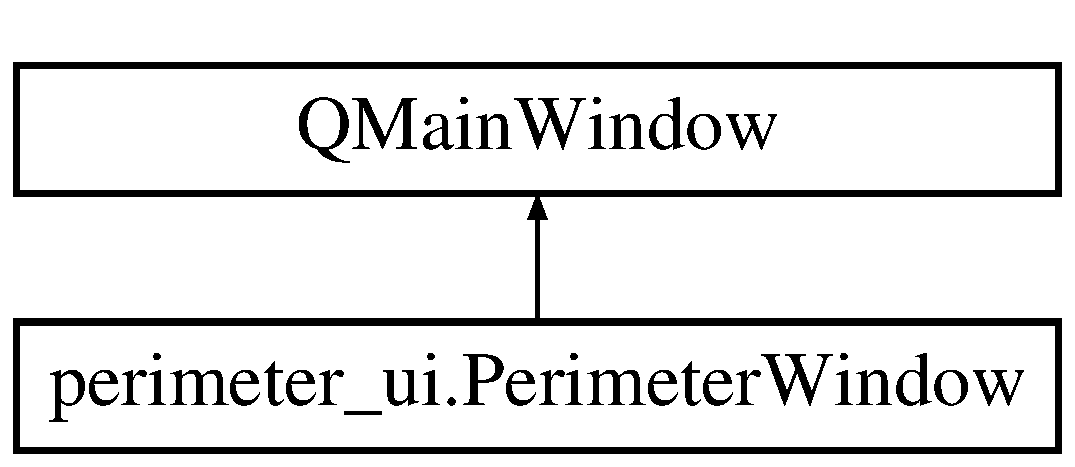
\includegraphics[height=2.000000cm]{classperimeter__ui_1_1_perimeter_window}
\end{center}
\end{figure}
\subsection*{Public Member Functions}
\begin{DoxyCompactItemize}
\item 
def \hyperlink{classperimeter__ui_1_1_perimeter_window_aa763b2caa5f3425d4666e237a58c1dc3}{\+\_\+\+\_\+init\+\_\+\+\_\+} (self, path=\char`\"{}\char`\"{})
\begin{DoxyCompactList}\small\item\em The constructor of the Perimeter window. \end{DoxyCompactList}\item 
def \hyperlink{classperimeter__ui_1_1_perimeter_window_afdeb1c9d24171741ae3077eaa4e2070d}{perimeter} (self)
\begin{DoxyCompactList}\small\item\em Displays the perimeter of selected shape given appropriate side lengths/radius. \end{DoxyCompactList}\item 
\mbox{\Hypertarget{classperimeter__ui_1_1_perimeter_window_a81461f899e536b3dc57a8bfda6f3ba01}\label{classperimeter__ui_1_1_perimeter_window_a81461f899e536b3dc57a8bfda6f3ba01}} 
def \hyperlink{classperimeter__ui_1_1_perimeter_window_a81461f899e536b3dc57a8bfda6f3ba01}{set\+Fields} (self)
\begin{DoxyCompactList}\small\item\em Changes and displays in text boxes corresponding to chosen shape. \end{DoxyCompactList}\item 
\mbox{\Hypertarget{classperimeter__ui_1_1_perimeter_window_a2e9715796974be96bdf58f6b9235e95f}\label{classperimeter__ui_1_1_perimeter_window_a2e9715796974be96bdf58f6b9235e95f}} 
def \hyperlink{classperimeter__ui_1_1_perimeter_window_a2e9715796974be96bdf58f6b9235e95f}{close\+Event} (self, event)
\begin{DoxyCompactList}\small\item\em Closes window and clears inputs upon close. \end{DoxyCompactList}\item 
\mbox{\Hypertarget{classperimeter__ui_1_1_perimeter_window_a19139d947ed5061dc53a29f1272fc51d}\label{classperimeter__ui_1_1_perimeter_window_a19139d947ed5061dc53a29f1272fc51d}} 
def \hyperlink{classperimeter__ui_1_1_perimeter_window_a19139d947ed5061dc53a29f1272fc51d}{clear\+Fields} (self)
\begin{DoxyCompactList}\small\item\em Clears all input and output fields. \end{DoxyCompactList}\end{DoxyCompactItemize}
\subsection*{Public Attributes}
\begin{DoxyCompactItemize}
\item 
\mbox{\Hypertarget{classperimeter__ui_1_1_perimeter_window_aa5f7496d431ceed317466669c3051272}\label{classperimeter__ui_1_1_perimeter_window_aa5f7496d431ceed317466669c3051272}} 
{\bfseries path}
\end{DoxyCompactItemize}


\subsection{Detailed Description}
\hyperlink{classperimeter__ui_1_1_perimeter_window}{Perimeter\+Window} is a class that implements the G\+UI components for the Perimeter operation. 

\subsection{Constructor \& Destructor Documentation}
\mbox{\Hypertarget{classperimeter__ui_1_1_perimeter_window_aa763b2caa5f3425d4666e237a58c1dc3}\label{classperimeter__ui_1_1_perimeter_window_aa763b2caa5f3425d4666e237a58c1dc3}} 
\index{perimeter\+\_\+ui\+::\+Perimeter\+Window@{perimeter\+\_\+ui\+::\+Perimeter\+Window}!\+\_\+\+\_\+init\+\_\+\+\_\+@{\+\_\+\+\_\+init\+\_\+\+\_\+}}
\index{\+\_\+\+\_\+init\+\_\+\+\_\+@{\+\_\+\+\_\+init\+\_\+\+\_\+}!perimeter\+\_\+ui\+::\+Perimeter\+Window@{perimeter\+\_\+ui\+::\+Perimeter\+Window}}
\subsubsection{\texorpdfstring{\+\_\+\+\_\+init\+\_\+\+\_\+()}{\_\_init\_\_()}}
{\footnotesize\ttfamily def perimeter\+\_\+ui.\+Perimeter\+Window.\+\_\+\+\_\+init\+\_\+\+\_\+ (\begin{DoxyParamCaption}\item[{}]{self,  }\item[{}]{path = {\ttfamily \char`\"{}\char`\"{}} }\end{DoxyParamCaption})}



The constructor of the Perimeter window. 

Creates a pop up window that displays and sets up the buttons and input fields that are necessary to obtain input from the user and calculate the appropriate answer. Also sets up the window according to the created style sheet. 
\begin{DoxyParams}{Parameters}
{\em path} & The current path on which the file is found. Default value is an empty path. \\
\hline
\end{DoxyParams}


\subsection{Member Function Documentation}
\mbox{\Hypertarget{classperimeter__ui_1_1_perimeter_window_afdeb1c9d24171741ae3077eaa4e2070d}\label{classperimeter__ui_1_1_perimeter_window_afdeb1c9d24171741ae3077eaa4e2070d}} 
\index{perimeter\+\_\+ui\+::\+Perimeter\+Window@{perimeter\+\_\+ui\+::\+Perimeter\+Window}!perimeter@{perimeter}}
\index{perimeter@{perimeter}!perimeter\+\_\+ui\+::\+Perimeter\+Window@{perimeter\+\_\+ui\+::\+Perimeter\+Window}}
\subsubsection{\texorpdfstring{perimeter()}{perimeter()}}
{\footnotesize\ttfamily def perimeter\+\_\+ui.\+Perimeter\+Window.\+perimeter (\begin{DoxyParamCaption}\item[{}]{self }\end{DoxyParamCaption})}



Displays the perimeter of selected shape given appropriate side lengths/radius. 

Takes in up to 3 side lengths and a radius as input from the user through input fields, and shows the user the result on the window 

The documentation for this class was generated from the following file\+:\begin{DoxyCompactItemize}
\item 
src/uis/\hyperlink{perimeter__ui_8py}{perimeter\+\_\+ui.\+py}\end{DoxyCompactItemize}

\hypertarget{classpythagore__ui_1_1_pytha_window}{}\section{pythagore\+\_\+ui.\+Pytha\+Window Class Reference}
\label{classpythagore__ui_1_1_pytha_window}\index{pythagore\+\_\+ui.\+Pytha\+Window@{pythagore\+\_\+ui.\+Pytha\+Window}}


\hyperlink{classpythagore__ui_1_1_pytha_window}{Pytha\+Window} is a class that implements the G\+UI components for the Pythagorean Theorem operation.  


Inheritance diagram for pythagore\+\_\+ui.\+Pytha\+Window\+:\begin{figure}[H]
\begin{center}
\leavevmode
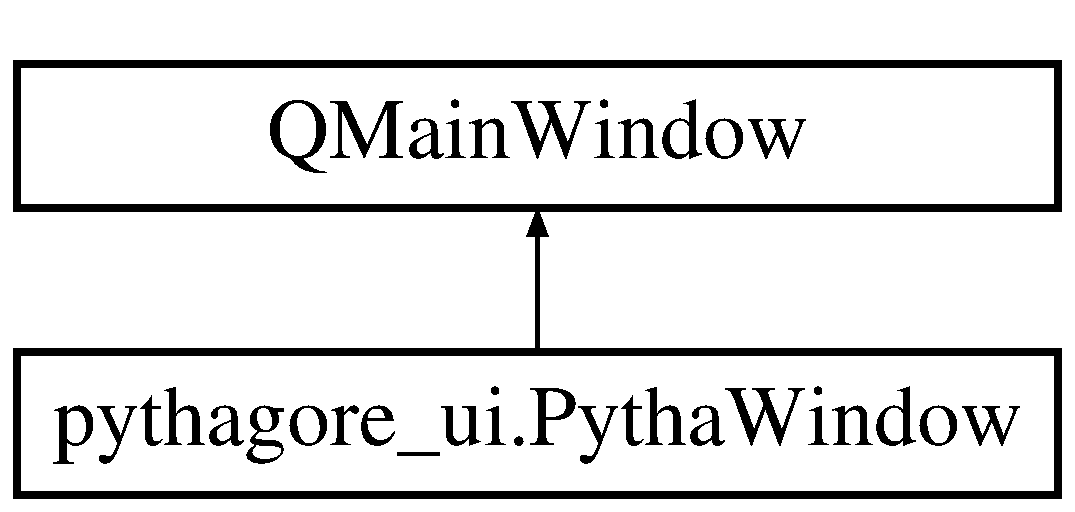
\includegraphics[height=2.000000cm]{classpythagore__ui_1_1_pytha_window}
\end{center}
\end{figure}
\subsection*{Public Member Functions}
\begin{DoxyCompactItemize}
\item 
def \hyperlink{classpythagore__ui_1_1_pytha_window_a3a9be6ba9c7645923a6e2a9eba16aa23}{\+\_\+\+\_\+init\+\_\+\+\_\+} (self, path=\char`\"{}\char`\"{})
\begin{DoxyCompactList}\small\item\em The constructor of the Pythagorean Theorem window. \end{DoxyCompactList}\item 
def \hyperlink{classpythagore__ui_1_1_pytha_window_accb4cda1de730c8001b0856b8327700a}{pytha} (self)
\begin{DoxyCompactList}\small\item\em Displays the length of the missing side of a right angle triangle. \end{DoxyCompactList}\end{DoxyCompactItemize}
\subsection*{Public Attributes}
\begin{DoxyCompactItemize}
\item 
\mbox{\Hypertarget{classpythagore__ui_1_1_pytha_window_a250c9e50d023f6a7344b10e87e57badf}\label{classpythagore__ui_1_1_pytha_window_a250c9e50d023f6a7344b10e87e57badf}} 
{\bfseries path}
\end{DoxyCompactItemize}


\subsection{Detailed Description}
\hyperlink{classpythagore__ui_1_1_pytha_window}{Pytha\+Window} is a class that implements the G\+UI components for the Pythagorean Theorem operation. 

\subsection{Constructor \& Destructor Documentation}
\mbox{\Hypertarget{classpythagore__ui_1_1_pytha_window_a3a9be6ba9c7645923a6e2a9eba16aa23}\label{classpythagore__ui_1_1_pytha_window_a3a9be6ba9c7645923a6e2a9eba16aa23}} 
\index{pythagore\+\_\+ui\+::\+Pytha\+Window@{pythagore\+\_\+ui\+::\+Pytha\+Window}!\+\_\+\+\_\+init\+\_\+\+\_\+@{\+\_\+\+\_\+init\+\_\+\+\_\+}}
\index{\+\_\+\+\_\+init\+\_\+\+\_\+@{\+\_\+\+\_\+init\+\_\+\+\_\+}!pythagore\+\_\+ui\+::\+Pytha\+Window@{pythagore\+\_\+ui\+::\+Pytha\+Window}}
\subsubsection{\texorpdfstring{\+\_\+\+\_\+init\+\_\+\+\_\+()}{\_\_init\_\_()}}
{\footnotesize\ttfamily def pythagore\+\_\+ui.\+Pytha\+Window.\+\_\+\+\_\+init\+\_\+\+\_\+ (\begin{DoxyParamCaption}\item[{}]{self,  }\item[{}]{path = {\ttfamily \char`\"{}\char`\"{}} }\end{DoxyParamCaption})}



The constructor of the Pythagorean Theorem window. 

Creates a pop up window that displays and sets up the buttons and input fields that are necessary to obtain input from the user and calculate the appropriate answer. Also sets up the window according to the created style sheet. 
\begin{DoxyParams}{Parameters}
{\em path} & The current path on which the file is found. Default value is an empty path. \\
\hline
\end{DoxyParams}


\subsection{Member Function Documentation}
\mbox{\Hypertarget{classpythagore__ui_1_1_pytha_window_accb4cda1de730c8001b0856b8327700a}\label{classpythagore__ui_1_1_pytha_window_accb4cda1de730c8001b0856b8327700a}} 
\index{pythagore\+\_\+ui\+::\+Pytha\+Window@{pythagore\+\_\+ui\+::\+Pytha\+Window}!pytha@{pytha}}
\index{pytha@{pytha}!pythagore\+\_\+ui\+::\+Pytha\+Window@{pythagore\+\_\+ui\+::\+Pytha\+Window}}
\subsubsection{\texorpdfstring{pytha()}{pytha()}}
{\footnotesize\ttfamily def pythagore\+\_\+ui.\+Pytha\+Window.\+pytha (\begin{DoxyParamCaption}\item[{}]{self }\end{DoxyParamCaption})}



Displays the length of the missing side of a right angle triangle. 

Takes the inputs of two sides from the user through input fields, and shows the user the length of the missing side on the window 

The documentation for this class was generated from the following file\+:\begin{DoxyCompactItemize}
\item 
src/uis/\hyperlink{pythagore__ui_8py}{pythagore\+\_\+ui.\+py}\end{DoxyCompactItemize}

\hypertarget{classstock__ui_1_1_stock_window}{}\section{stock\+\_\+ui.\+Stock\+Window Class Reference}
\label{classstock__ui_1_1_stock_window}\index{stock\+\_\+ui.\+Stock\+Window@{stock\+\_\+ui.\+Stock\+Window}}


\hyperlink{classstock__ui_1_1_stock_window}{Stock\+Window} is a class that implements the G\+UI components for the Stock operation menu.  


Inheritance diagram for stock\+\_\+ui.\+Stock\+Window\+:\begin{figure}[H]
\begin{center}
\leavevmode
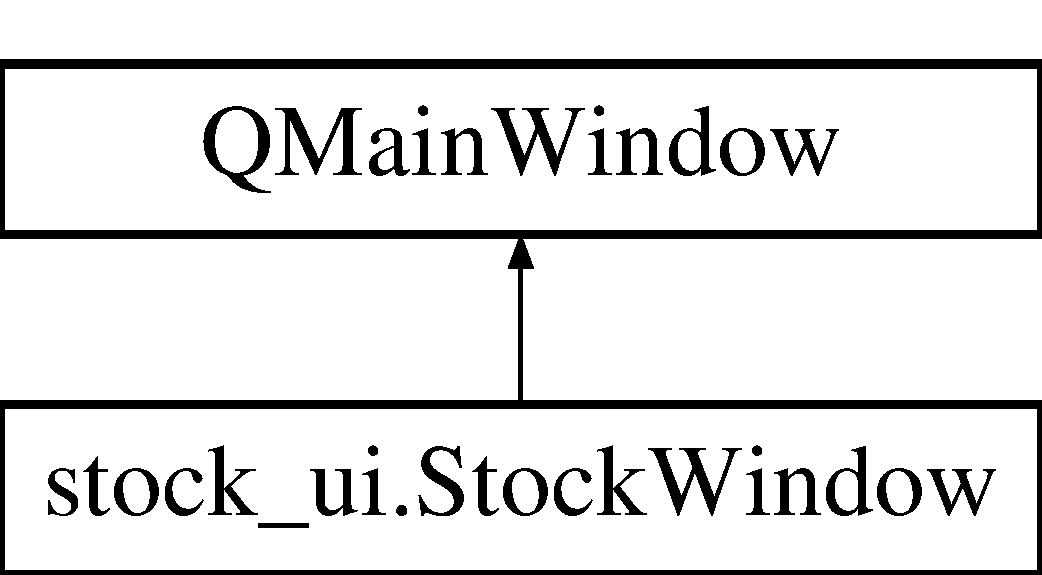
\includegraphics[height=2.000000cm]{classstock__ui_1_1_stock_window}
\end{center}
\end{figure}
\subsection*{Public Member Functions}
\begin{DoxyCompactItemize}
\item 
def \hyperlink{classstock__ui_1_1_stock_window_a7347eaa350a1387847c614c65ef35718}{\+\_\+\+\_\+init\+\_\+\+\_\+} (self, path=\char`\"{}\char`\"{})
\begin{DoxyCompactList}\small\item\em The constructor of the Stock window. \end{DoxyCompactList}\item 
def \hyperlink{classstock__ui_1_1_stock_window_a81a932663d0fdf4674729367ce8f5d4e}{stock} (self)
\begin{DoxyCompactList}\small\item\em Displays the loss or gain on the stock from the metrics the user provides. \end{DoxyCompactList}\end{DoxyCompactItemize}
\subsection*{Public Attributes}
\begin{DoxyCompactItemize}
\item 
\mbox{\Hypertarget{classstock__ui_1_1_stock_window_a799b895206dbff001bcc12929d0af1ce}\label{classstock__ui_1_1_stock_window_a799b895206dbff001bcc12929d0af1ce}} 
{\bfseries path}
\end{DoxyCompactItemize}


\subsection{Detailed Description}
\hyperlink{classstock__ui_1_1_stock_window}{Stock\+Window} is a class that implements the G\+UI components for the Stock operation menu. 

\subsection{Constructor \& Destructor Documentation}
\mbox{\Hypertarget{classstock__ui_1_1_stock_window_a7347eaa350a1387847c614c65ef35718}\label{classstock__ui_1_1_stock_window_a7347eaa350a1387847c614c65ef35718}} 
\index{stock\+\_\+ui\+::\+Stock\+Window@{stock\+\_\+ui\+::\+Stock\+Window}!\+\_\+\+\_\+init\+\_\+\+\_\+@{\+\_\+\+\_\+init\+\_\+\+\_\+}}
\index{\+\_\+\+\_\+init\+\_\+\+\_\+@{\+\_\+\+\_\+init\+\_\+\+\_\+}!stock\+\_\+ui\+::\+Stock\+Window@{stock\+\_\+ui\+::\+Stock\+Window}}
\subsubsection{\texorpdfstring{\+\_\+\+\_\+init\+\_\+\+\_\+()}{\_\_init\_\_()}}
{\footnotesize\ttfamily def stock\+\_\+ui.\+Stock\+Window.\+\_\+\+\_\+init\+\_\+\+\_\+ (\begin{DoxyParamCaption}\item[{}]{self,  }\item[{}]{path = {\ttfamily \char`\"{}\char`\"{}} }\end{DoxyParamCaption})}



The constructor of the Stock window. 

Creates a pop up window that displays and sets up the buttons that are necessary to navigate from the Stocks window to other parts of the application. Also sets up the Stocks window according to the created style sheet. 
\begin{DoxyParams}{Parameters}
{\em path} & The current path on which the file is found. Default value is an empty path. \\
\hline
\end{DoxyParams}


\subsection{Member Function Documentation}
\mbox{\Hypertarget{classstock__ui_1_1_stock_window_a81a932663d0fdf4674729367ce8f5d4e}\label{classstock__ui_1_1_stock_window_a81a932663d0fdf4674729367ce8f5d4e}} 
\index{stock\+\_\+ui\+::\+Stock\+Window@{stock\+\_\+ui\+::\+Stock\+Window}!stock@{stock}}
\index{stock@{stock}!stock\+\_\+ui\+::\+Stock\+Window@{stock\+\_\+ui\+::\+Stock\+Window}}
\subsubsection{\texorpdfstring{stock()}{stock()}}
{\footnotesize\ttfamily def stock\+\_\+ui.\+Stock\+Window.\+stock (\begin{DoxyParamCaption}\item[{}]{self }\end{DoxyParamCaption})}



Displays the loss or gain on the stock from the metrics the user provides. 

Takes in the number of shares, purchase price, sell price, purchase commission and sell commission, through input fields, and shows the user the result on the window 

The documentation for this class was generated from the following file\+:\begin{DoxyCompactItemize}
\item 
src/uis/\hyperlink{stock__ui_8py}{stock\+\_\+ui.\+py}\end{DoxyCompactItemize}

\hypertarget{classvolume__ui_1_1_volume_window}{}\section{volume\+\_\+ui.\+Volume\+Window Class Reference}
\label{classvolume__ui_1_1_volume_window}\index{volume\+\_\+ui.\+Volume\+Window@{volume\+\_\+ui.\+Volume\+Window}}


\hyperlink{classvolume__ui_1_1_volume_window}{Volume\+Window} is a class that implements the G\+UI components for the Volume operation.  


Inheritance diagram for volume\+\_\+ui.\+Volume\+Window\+:\begin{figure}[H]
\begin{center}
\leavevmode
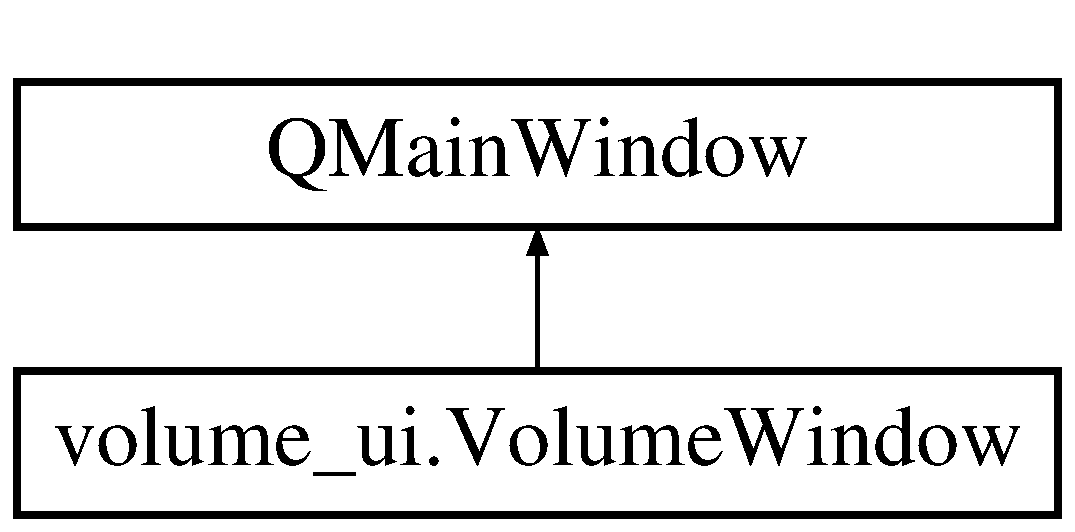
\includegraphics[height=2.000000cm]{classvolume__ui_1_1_volume_window}
\end{center}
\end{figure}
\subsection*{Public Member Functions}
\begin{DoxyCompactItemize}
\item 
def \hyperlink{classvolume__ui_1_1_volume_window_ab2ab926742b93b5fc0030332e60d4bc7}{\+\_\+\+\_\+init\+\_\+\+\_\+} (self, path=\char`\"{}\char`\"{})
\begin{DoxyCompactList}\small\item\em The constructor of the Volume window. \end{DoxyCompactList}\item 
def \hyperlink{classvolume__ui_1_1_volume_window_a1b4cb7b0bd52c5898a39dbfb81e5cb85}{volume} (self)
\begin{DoxyCompactList}\small\item\em Displays the volume of selected 3D shape given appropriate dimensions. \end{DoxyCompactList}\item 
\mbox{\Hypertarget{classvolume__ui_1_1_volume_window_a54f4caafa94056dcb90403c976c6d4b3}\label{classvolume__ui_1_1_volume_window_a54f4caafa94056dcb90403c976c6d4b3}} 
def \hyperlink{classvolume__ui_1_1_volume_window_a54f4caafa94056dcb90403c976c6d4b3}{set\+Fields} (self)
\begin{DoxyCompactList}\small\item\em Changes and displays in text boxes corresponding to chosen shape. \end{DoxyCompactList}\item 
\mbox{\Hypertarget{classvolume__ui_1_1_volume_window_ac1944f0385020e7c420f777d9c60b6df}\label{classvolume__ui_1_1_volume_window_ac1944f0385020e7c420f777d9c60b6df}} 
def \hyperlink{classvolume__ui_1_1_volume_window_ac1944f0385020e7c420f777d9c60b6df}{close\+Event} (self, event)
\begin{DoxyCompactList}\small\item\em Closes window and clears inputs upon close. \end{DoxyCompactList}\item 
\mbox{\Hypertarget{classvolume__ui_1_1_volume_window_a6c2e9282cb113a4b635719d5e3b2e80a}\label{classvolume__ui_1_1_volume_window_a6c2e9282cb113a4b635719d5e3b2e80a}} 
def \hyperlink{classvolume__ui_1_1_volume_window_a6c2e9282cb113a4b635719d5e3b2e80a}{clear\+Fields} (self)
\begin{DoxyCompactList}\small\item\em Clears all input and output fields. \end{DoxyCompactList}\end{DoxyCompactItemize}
\subsection*{Public Attributes}
\begin{DoxyCompactItemize}
\item 
\mbox{\Hypertarget{classvolume__ui_1_1_volume_window_ac1968ad0245de90cc4efb39c682d77b1}\label{classvolume__ui_1_1_volume_window_ac1968ad0245de90cc4efb39c682d77b1}} 
{\bfseries path}
\end{DoxyCompactItemize}


\subsection{Detailed Description}
\hyperlink{classvolume__ui_1_1_volume_window}{Volume\+Window} is a class that implements the G\+UI components for the Volume operation. 

\subsection{Constructor \& Destructor Documentation}
\mbox{\Hypertarget{classvolume__ui_1_1_volume_window_ab2ab926742b93b5fc0030332e60d4bc7}\label{classvolume__ui_1_1_volume_window_ab2ab926742b93b5fc0030332e60d4bc7}} 
\index{volume\+\_\+ui\+::\+Volume\+Window@{volume\+\_\+ui\+::\+Volume\+Window}!\+\_\+\+\_\+init\+\_\+\+\_\+@{\+\_\+\+\_\+init\+\_\+\+\_\+}}
\index{\+\_\+\+\_\+init\+\_\+\+\_\+@{\+\_\+\+\_\+init\+\_\+\+\_\+}!volume\+\_\+ui\+::\+Volume\+Window@{volume\+\_\+ui\+::\+Volume\+Window}}
\subsubsection{\texorpdfstring{\+\_\+\+\_\+init\+\_\+\+\_\+()}{\_\_init\_\_()}}
{\footnotesize\ttfamily def volume\+\_\+ui.\+Volume\+Window.\+\_\+\+\_\+init\+\_\+\+\_\+ (\begin{DoxyParamCaption}\item[{}]{self,  }\item[{}]{path = {\ttfamily \char`\"{}\char`\"{}} }\end{DoxyParamCaption})}



The constructor of the Volume window. 

Creates a pop up window that displays and sets up the buttons and input fields that are necessary to obtain input from the user and calculate the appropriate answer. Also sets up the window according to the created style sheet. 
\begin{DoxyParams}{Parameters}
{\em path} & The current path on which the file is found. Default value is an empty path. \\
\hline
\end{DoxyParams}


\subsection{Member Function Documentation}
\mbox{\Hypertarget{classvolume__ui_1_1_volume_window_a1b4cb7b0bd52c5898a39dbfb81e5cb85}\label{classvolume__ui_1_1_volume_window_a1b4cb7b0bd52c5898a39dbfb81e5cb85}} 
\index{volume\+\_\+ui\+::\+Volume\+Window@{volume\+\_\+ui\+::\+Volume\+Window}!volume@{volume}}
\index{volume@{volume}!volume\+\_\+ui\+::\+Volume\+Window@{volume\+\_\+ui\+::\+Volume\+Window}}
\subsubsection{\texorpdfstring{volume()}{volume()}}
{\footnotesize\ttfamily def volume\+\_\+ui.\+Volume\+Window.\+volume (\begin{DoxyParamCaption}\item[{}]{self }\end{DoxyParamCaption})}



Displays the volume of selected 3D shape given appropriate dimensions. 

Takes in up to 3 dimensions and/or radius as input from the user through input fields, and shows the user the result on the window 

The documentation for this class was generated from the following file\+:\begin{DoxyCompactItemize}
\item 
src/uis/\hyperlink{volume__ui_8py}{volume\+\_\+ui.\+py}\end{DoxyCompactItemize}

\chapter{File Documentation}
\hypertarget{main_8py}{}\section{src/main.py File Reference}
\label{main_8py}\index{src/main.\+py@{src/main.\+py}}


Provides a class to display the Main window.  


\subsection*{Classes}
\begin{DoxyCompactItemize}
\item 
class \hyperlink{classmain_1_1_main_window}{main.\+Main\+Window}
\begin{DoxyCompactList}\small\item\em \hyperlink{classmain_1_1_main_window}{Main\+Window} is a class that implements the G\+UI components for the Main menu. \end{DoxyCompactList}\end{DoxyCompactItemize}
\subsection*{Functions}
\begin{DoxyCompactItemize}
\item 
\mbox{\Hypertarget{main_8py_a72b3d1c789929c5800f3adc8c4b83435}\label{main_8py_a72b3d1c789929c5800f3adc8c4b83435}} 
def {\bfseries main.\+start\+\_\+gui} ()
\end{DoxyCompactItemize}


\subsection{Detailed Description}
Provides a class to display the Main window. 

\begin{DoxyDate}{Date}
March 30, 2022 
\end{DoxyDate}

\hypertarget{algebra__ui_8py}{}\section{src/uis/algebra\+\_\+ui.py File Reference}
\label{algebra__ui_8py}\index{src/uis/algebra\+\_\+ui.\+py@{src/uis/algebra\+\_\+ui.\+py}}


Provides a class to display the Algebra window.  


\subsection*{Classes}
\begin{DoxyCompactItemize}
\item 
class \hyperlink{classalgebra__ui_1_1_algebra_window}{algebra\+\_\+ui.\+Algebra\+Window}
\begin{DoxyCompactList}\small\item\em \hyperlink{classalgebra__ui_1_1_algebra_window}{Algebra\+Window} is a class that implements the G\+UI components for the Algebra operation menu. \end{DoxyCompactList}\end{DoxyCompactItemize}
\subsection*{Variables}
\begin{DoxyCompactItemize}
\item 
\mbox{\Hypertarget{algebra__ui_8py_ace33e95684b9942633115627153249d6}\label{algebra__ui_8py_ace33e95684b9942633115627153249d6}} 
{\bfseries algebra\+\_\+ui.\+app} = Q\+Application(sys.\+argv)
\item 
\mbox{\Hypertarget{algebra__ui_8py_aa507164f7e27706bf97436631a992d6b}\label{algebra__ui_8py_aa507164f7e27706bf97436631a992d6b}} 
{\bfseries algebra\+\_\+ui.\+window} = Algebra\+Window()
\end{DoxyCompactItemize}


\subsection{Detailed Description}
Provides a class to display the Algebra window. 

\begin{DoxyDate}{Date}
March 30, 2022 
\end{DoxyDate}

\hypertarget{area__ui_8py}{}\section{src/uis/area\+\_\+ui.py File Reference}
\label{area__ui_8py}\index{src/uis/area\+\_\+ui.\+py@{src/uis/area\+\_\+ui.\+py}}


Provides a class to display the Area window.  


\subsection*{Classes}
\begin{DoxyCompactItemize}
\item 
class \hyperlink{classarea__ui_1_1_area_window}{area\+\_\+ui.\+Area\+Window}
\begin{DoxyCompactList}\small\item\em \hyperlink{classarea__ui_1_1_area_window}{Area\+Window} is a class that implements the G\+UI components for the Area operation. \end{DoxyCompactList}\end{DoxyCompactItemize}
\subsection*{Variables}
\begin{DoxyCompactItemize}
\item 
\mbox{\Hypertarget{area__ui_8py_a65091aeb348bfb6475364b7a68892750}\label{area__ui_8py_a65091aeb348bfb6475364b7a68892750}} 
{\bfseries area\+\_\+ui.\+app} = Q\+Application(sys.\+argv)
\item 
\mbox{\Hypertarget{area__ui_8py_a31e0599bf3aa69539baba5e1c91d45a0}\label{area__ui_8py_a31e0599bf3aa69539baba5e1c91d45a0}} 
{\bfseries area\+\_\+ui.\+window} = Area\+Window()
\end{DoxyCompactItemize}


\subsection{Detailed Description}
Provides a class to display the Area window. 

\begin{DoxyDate}{Date}
March 18, 2022 
\end{DoxyDate}

\hypertarget{binary__arithmetic__ui_8py}{}\section{src/uis/binary\+\_\+arithmetic\+\_\+ui.py File Reference}
\label{binary__arithmetic__ui_8py}\index{src/uis/binary\+\_\+arithmetic\+\_\+ui.\+py@{src/uis/binary\+\_\+arithmetic\+\_\+ui.\+py}}


Provides a class to display the Binary Arithmetic window.  


\subsection*{Classes}
\begin{DoxyCompactItemize}
\item 
class \hyperlink{classbinary__arithmetic__ui_1_1_bin_arithmetic_window}{binary\+\_\+arithmetic\+\_\+ui.\+Bin\+Arithmetic\+Window}
\begin{DoxyCompactList}\small\item\em \hyperlink{classbinary__arithmetic__ui_1_1_bin_arithmetic_window}{Bin\+Arithmetic\+Window} is a class that implements the G\+UI components for the Binary Arithmetic operations. \end{DoxyCompactList}\end{DoxyCompactItemize}
\subsection*{Variables}
\begin{DoxyCompactItemize}
\item 
\mbox{\Hypertarget{binary__arithmetic__ui_8py_ac2d197dfa3395a701c417f6963ba8666}\label{binary__arithmetic__ui_8py_ac2d197dfa3395a701c417f6963ba8666}} 
{\bfseries binary\+\_\+arithmetic\+\_\+ui.\+app} = Q\+Application(sys.\+argv)
\item 
\mbox{\Hypertarget{binary__arithmetic__ui_8py_aedb9fb98322759146e12a038d58c32d9}\label{binary__arithmetic__ui_8py_aedb9fb98322759146e12a038d58c32d9}} 
{\bfseries binary\+\_\+arithmetic\+\_\+ui.\+window} = Bin\+Arithmetic\+Window()
\end{DoxyCompactItemize}


\subsection{Detailed Description}
Provides a class to display the Binary Arithmetic window. 

\begin{DoxyDate}{Date}
March 18, 2022 
\end{DoxyDate}

\hypertarget{binary__ui_8py}{}\section{src/uis/binary\+\_\+ui.py File Reference}
\label{binary__ui_8py}\index{src/uis/binary\+\_\+ui.\+py@{src/uis/binary\+\_\+ui.\+py}}


Provides a class to display the Binary window.  


\subsection*{Classes}
\begin{DoxyCompactItemize}
\item 
class \hyperlink{classbinary__ui_1_1_binary_window}{binary\+\_\+ui.\+Binary\+Window}
\begin{DoxyCompactList}\small\item\em \hyperlink{classbinary__ui_1_1_binary_window}{Binary\+Window} is a class that implements the G\+UI components for the Binary operation menu. \end{DoxyCompactList}\end{DoxyCompactItemize}
\subsection*{Variables}
\begin{DoxyCompactItemize}
\item 
\mbox{\Hypertarget{binary__ui_8py_a812f56b9f6981e04fbefa5d50ccaa68c}\label{binary__ui_8py_a812f56b9f6981e04fbefa5d50ccaa68c}} 
{\bfseries binary\+\_\+ui.\+app} = Q\+Application(sys.\+argv)
\item 
\mbox{\Hypertarget{binary__ui_8py_a10c86cc977000fe3129b12c39d7f1d1d}\label{binary__ui_8py_a10c86cc977000fe3129b12c39d7f1d1d}} 
{\bfseries binary\+\_\+ui.\+window} = Binary\+Window()
\end{DoxyCompactItemize}


\subsection{Detailed Description}
Provides a class to display the Binary window. 

\begin{DoxyDate}{Date}
March 18, 2022 
\end{DoxyDate}

\hypertarget{bitwise__ui_8py}{}\section{src/uis/bitwise\+\_\+ui.py File Reference}
\label{bitwise__ui_8py}\index{src/uis/bitwise\+\_\+ui.\+py@{src/uis/bitwise\+\_\+ui.\+py}}


Provides a class to display the Bitwise Operation window.  


\subsection*{Classes}
\begin{DoxyCompactItemize}
\item 
class \hyperlink{classbitwise__ui_1_1_bitwise_window}{bitwise\+\_\+ui.\+Bitwise\+Window}
\begin{DoxyCompactList}\small\item\em \hyperlink{classbitwise__ui_1_1_bitwise_window}{Bitwise\+Window} is a class that implements the G\+UI components for the Bitwise operations. \end{DoxyCompactList}\end{DoxyCompactItemize}
\subsection*{Variables}
\begin{DoxyCompactItemize}
\item 
\mbox{\Hypertarget{bitwise__ui_8py_aab93c14edc8b779f528e618bdae84003}\label{bitwise__ui_8py_aab93c14edc8b779f528e618bdae84003}} 
{\bfseries bitwise\+\_\+ui.\+app} = Q\+Application(sys.\+argv)
\item 
\mbox{\Hypertarget{bitwise__ui_8py_abe544969a493280fb101779cb782739f}\label{bitwise__ui_8py_abe544969a493280fb101779cb782739f}} 
{\bfseries bitwise\+\_\+ui.\+window} = Bitwise\+Window()
\end{DoxyCompactItemize}


\subsection{Detailed Description}
Provides a class to display the Bitwise Operation window. 

\begin{DoxyDate}{Date}
March 18, 2022 
\end{DoxyDate}

\hypertarget{_b_m_i__ui_8py}{}\section{src/uis/\+B\+M\+I\+\_\+ui.py File Reference}
\label{_b_m_i__ui_8py}\index{src/uis/\+B\+M\+I\+\_\+ui.\+py@{src/uis/\+B\+M\+I\+\_\+ui.\+py}}


Provides a class to display the B\+MI window.  


\subsection*{Classes}
\begin{DoxyCompactItemize}
\item 
class \hyperlink{class_b_m_i__ui_1_1_b_m_i_window}{B\+M\+I\+\_\+ui.\+B\+M\+I\+Window}
\begin{DoxyCompactList}\small\item\em \hyperlink{class_b_m_i__ui_1_1_b_m_i_window}{B\+M\+I\+Window} is a class that implements the G\+UI components for the B\+MI operation. \end{DoxyCompactList}\end{DoxyCompactItemize}
\subsection*{Variables}
\begin{DoxyCompactItemize}
\item 
\mbox{\Hypertarget{_b_m_i__ui_8py_a47da8ca9f942eae1dd682ca2fb74f19b}\label{_b_m_i__ui_8py_a47da8ca9f942eae1dd682ca2fb74f19b}} 
{\bfseries B\+M\+I\+\_\+ui.\+app} = Q\+Application(sys.\+argv)
\item 
\mbox{\Hypertarget{_b_m_i__ui_8py_a5f0e00fadb8e7bf1733ed3a5e31c380e}\label{_b_m_i__ui_8py_a5f0e00fadb8e7bf1733ed3a5e31c380e}} 
{\bfseries B\+M\+I\+\_\+ui.\+window} = B\+M\+I\+Window()
\end{DoxyCompactItemize}


\subsection{Detailed Description}
Provides a class to display the B\+MI window. 

\begin{DoxyDate}{Date}
March 30, 2022 
\end{DoxyDate}

\hypertarget{_body_fat__ui_8py}{}\section{src/uis/\+Body\+Fat\+\_\+ui.py File Reference}
\label{_body_fat__ui_8py}\index{src/uis/\+Body\+Fat\+\_\+ui.\+py@{src/uis/\+Body\+Fat\+\_\+ui.\+py}}


Provides a class to display the Body Fat window.  


\subsection*{Classes}
\begin{DoxyCompactItemize}
\item 
class \hyperlink{class_body_fat__ui_1_1_b_f_window}{Body\+Fat\+\_\+ui.\+B\+F\+Window}
\begin{DoxyCompactList}\small\item\em \hyperlink{class_body_fat__ui_1_1_b_f_window}{B\+F\+Window} is a class that implements the G\+UI components for the Body Fat operation. \end{DoxyCompactList}\end{DoxyCompactItemize}
\subsection*{Variables}
\begin{DoxyCompactItemize}
\item 
\mbox{\Hypertarget{_body_fat__ui_8py_a812f4ffaa9caa695ee027110735d0315}\label{_body_fat__ui_8py_a812f4ffaa9caa695ee027110735d0315}} 
{\bfseries Body\+Fat\+\_\+ui.\+app} = Q\+Application(sys.\+argv)
\item 
\mbox{\Hypertarget{_body_fat__ui_8py_a46b2703080cd4eb6fca1212bc6bc69f7}\label{_body_fat__ui_8py_a46b2703080cd4eb6fca1212bc6bc69f7}} 
{\bfseries Body\+Fat\+\_\+ui.\+window} = B\+F\+Window()
\end{DoxyCompactItemize}


\subsection{Detailed Description}
Provides a class to display the Body Fat window. 

\begin{DoxyDate}{Date}
March 17, 2022 
\end{DoxyDate}

\hypertarget{algebra__calculator_8py}{}\section{src/uis/\+Calculators/algebra\+\_\+calculator.py File Reference}
\label{algebra__calculator_8py}\index{src/uis/\+Calculators/algebra\+\_\+calculator.\+py@{src/uis/\+Calculators/algebra\+\_\+calculator.\+py}}


Alegbraic algorithms.  


\subsection*{Functions}
\begin{DoxyCompactItemize}
\item 
def \hyperlink{algebra__calculator_8py_af935266ec6ad78528f1adeb4470de058}{algebra\+\_\+calculator.\+slope\+Of\+Line} (x1, y1, x2, y2)
\begin{DoxyCompactList}\small\item\em Calculates slope of a line given 2 points. \end{DoxyCompactList}\item 
def \hyperlink{algebra__calculator_8py_a163b051062c0e36b45b965acb80db74e}{algebra\+\_\+calculator.\+y\+Intercept} (m, x, y)
\begin{DoxyCompactList}\small\item\em Calculates y-\/intercept of a line given a point and the slope. \end{DoxyCompactList}\item 
def \hyperlink{algebra__calculator_8py_ac52e25ab6ce734116b28919d3f29da42}{algebra\+\_\+calculator.\+py\+Theorem} (solve, a, b, c)
\begin{DoxyCompactList}\small\item\em Calculates pythagorean theorem of a right triangle given two sides and the side to solve for. \end{DoxyCompactList}\end{DoxyCompactItemize}


\subsection{Detailed Description}
Alegbraic algorithms. 

\begin{DoxyDate}{Date}
March 17, 2022 
\end{DoxyDate}


\subsection{Function Documentation}
\mbox{\Hypertarget{algebra__calculator_8py_file_ac52e25ab6ce734116b28919d3f29da42}\label{algebra__calculator_8py_file_ac52e25ab6ce734116b28919d3f29da42}} 
\index{algebra\+\_\+calculator.\+py@{algebra\+\_\+calculator.\+py}!py\+Theorem@{py\+Theorem}}
\index{py\+Theorem@{py\+Theorem}!algebra\+\_\+calculator.\+py@{algebra\+\_\+calculator.\+py}}
\subsubsection{\texorpdfstring{py\+Theorem()}{pyTheorem()}}
{\footnotesize\ttfamily def algebra\+\_\+calculator.\+py\+Theorem (\begin{DoxyParamCaption}\item[{}]{solve,  }\item[{}]{a,  }\item[{}]{b,  }\item[{}]{c }\end{DoxyParamCaption})}



Calculates pythagorean theorem of a right triangle given two sides and the side to solve for. 


\begin{DoxyParams}{Parameters}
{\em solve} & A string that represents the missing side \\
\hline
{\em a} & A real number that represents a side the is not the hypotenuse \\
\hline
{\em b} & A real number that represents a side the is not the hypotenuse \\
\hline
{\em c} & A real number that represents the hypotenuse \\
\hline
\end{DoxyParams}
\begin{DoxyReturn}{Returns}
The length of the missing side 
\end{DoxyReturn}

\begin{DoxyExceptions}{Exceptions}
{\em Value\+Error} & Throws an exception if hypotenuse is not the longest side or sides are not postive \\
\hline
\end{DoxyExceptions}
\mbox{\Hypertarget{algebra__calculator_8py_file_af935266ec6ad78528f1adeb4470de058}\label{algebra__calculator_8py_file_af935266ec6ad78528f1adeb4470de058}} 
\index{algebra\+\_\+calculator.\+py@{algebra\+\_\+calculator.\+py}!slope\+Of\+Line@{slope\+Of\+Line}}
\index{slope\+Of\+Line@{slope\+Of\+Line}!algebra\+\_\+calculator.\+py@{algebra\+\_\+calculator.\+py}}
\subsubsection{\texorpdfstring{slope\+Of\+Line()}{slopeOfLine()}}
{\footnotesize\ttfamily def algebra\+\_\+calculator.\+slope\+Of\+Line (\begin{DoxyParamCaption}\item[{}]{x1,  }\item[{}]{y1,  }\item[{}]{x2,  }\item[{}]{y2 }\end{DoxyParamCaption})}



Calculates slope of a line given 2 points. 


\begin{DoxyParams}{Parameters}
{\em x1} & A real number that represents the X-\/coordinate of the first point \\
\hline
{\em y1} & A real number that represents the Y-\/coordinate of the first point \\
\hline
{\em x2} & A real number that represents the X-\/coordinate of the second point \\
\hline
{\em y2} & A real number that represents the Y-\/coordinate of the second point \\
\hline
\end{DoxyParams}
\begin{DoxyReturn}{Returns}
The slope of the line 
\end{DoxyReturn}

\begin{DoxyExceptions}{Exceptions}
{\em Zero\+Division\+Error} & Throws an exception if x2 and x1 are equal \\
\hline
\end{DoxyExceptions}
\mbox{\Hypertarget{algebra__calculator_8py_file_a163b051062c0e36b45b965acb80db74e}\label{algebra__calculator_8py_file_a163b051062c0e36b45b965acb80db74e}} 
\index{algebra\+\_\+calculator.\+py@{algebra\+\_\+calculator.\+py}!y\+Intercept@{y\+Intercept}}
\index{y\+Intercept@{y\+Intercept}!algebra\+\_\+calculator.\+py@{algebra\+\_\+calculator.\+py}}
\subsubsection{\texorpdfstring{y\+Intercept()}{yIntercept()}}
{\footnotesize\ttfamily def algebra\+\_\+calculator.\+y\+Intercept (\begin{DoxyParamCaption}\item[{}]{m,  }\item[{}]{x,  }\item[{}]{y }\end{DoxyParamCaption})}



Calculates y-\/intercept of a line given a point and the slope. 


\begin{DoxyParams}{Parameters}
{\em m} & A real number that represents the slope of the line \\
\hline
{\em x} & A real number that represents the X-\/coordinate of the point \\
\hline
{\em y} & A real number that represents the Y-\/coordinate of the point \\
\hline
\end{DoxyParams}
\begin{DoxyReturn}{Returns}
The y-\/intercept of the line 
\end{DoxyReturn}

\hypertarget{binary__calculator_8py}{}\section{src/uis/\+Calculators/binary\+\_\+calculator.py File Reference}
\label{binary__calculator_8py}\index{src/uis/\+Calculators/binary\+\_\+calculator.\+py@{src/uis/\+Calculators/binary\+\_\+calculator.\+py}}


Binary algorithms.  


\subsection*{Functions}
\begin{DoxyCompactItemize}
\item 
def \hyperlink{binary__calculator_8py_aa4e5bd7c4a514c592fdbbc8d39d8db96}{binary\+\_\+calculator.\+to\+Floating\+Point} (n)
\begin{DoxyCompactList}\small\item\em Calculates I\+E\+EE 754 representation from decimal. \end{DoxyCompactList}\item 
def \hyperlink{binary__calculator_8py_a37f2266dbd95f438fe1293cb63e95fb8}{binary\+\_\+calculator.\+to\+Decimal} (n)
\begin{DoxyCompactList}\small\item\em Calculates decimal number from I\+E\+EE 754 representation. \end{DoxyCompactList}\item 
def \hyperlink{binary__calculator_8py_af7c77202b99b2d5558b445897258618b}{binary\+\_\+calculator.\+bin\+Add} (n, m)
\begin{DoxyCompactList}\small\item\em Calculates sum of two binary numbers. \end{DoxyCompactList}\item 
def \hyperlink{binary__calculator_8py_ad358d6e67ec21ec1025cce2183d491c9}{binary\+\_\+calculator.\+bin\+Sub} (n, m)
\begin{DoxyCompactList}\small\item\em Calculates difference of two binary numbers. \end{DoxyCompactList}\item 
def \hyperlink{binary__calculator_8py_abaf092e6dab88e974807aff94f12c69c}{binary\+\_\+calculator.\+bin\+Mult} (n, m)
\begin{DoxyCompactList}\small\item\em Calculates product of two binary numbers. \end{DoxyCompactList}\item 
def \hyperlink{binary__calculator_8py_a58deaaed29571302dbfd68c22b615752}{binary\+\_\+calculator.\+bin\+Div} (n, m)
\begin{DoxyCompactList}\small\item\em Calculates quotient of two binary numbers. \end{DoxyCompactList}\item 
def \hyperlink{binary__calculator_8py_af14cdd065d797225bd7de45af097e4f0}{binary\+\_\+calculator.\+bin\+Pow} (n, m)
\begin{DoxyCompactList}\small\item\em Calculates power of two binary numbers. \end{DoxyCompactList}\item 
def \hyperlink{binary__calculator_8py_a86fde77c9b817c5c479d5e93002e665f}{binary\+\_\+calculator.\+bitwise\+A\+ND} (n, m)
\begin{DoxyCompactList}\small\item\em Calculates bitwise A\+ND of two binary numbers. \end{DoxyCompactList}\item 
def \hyperlink{binary__calculator_8py_ac50101951e276bd216cd18308a787017}{binary\+\_\+calculator.\+bitwise\+OR} (n, m)
\begin{DoxyCompactList}\small\item\em Calculates bitwise OR of two binary numbers. \end{DoxyCompactList}\item 
def \hyperlink{binary__calculator_8py_adce8c6311d8ee4277160441895d40690}{binary\+\_\+calculator.\+bitwise\+N\+OT} (n)
\begin{DoxyCompactList}\small\item\em Calculates bitwise N\+OT of binary number. \end{DoxyCompactList}\item 
def \hyperlink{binary__calculator_8py_a7a660a915ab78adc909c6aa761d18d00}{binary\+\_\+calculator.\+bitwise\+X\+OR} (n, m)
\begin{DoxyCompactList}\small\item\em Calculates bitwise X\+OR of two binary numbers. \end{DoxyCompactList}\item 
def \hyperlink{binary__calculator_8py_af2cbf28fec66013a8b1ba1b3f0f548e2}{binary\+\_\+calculator.\+rshift} (n, shift\+Num, length)
\begin{DoxyCompactList}\small\item\em Calculates rightward bit shift of binary number using given shift number and length. \end{DoxyCompactList}\item 
def \hyperlink{binary__calculator_8py_af9c9d478f3f4476bf7fb363a622f7ca7}{binary\+\_\+calculator.\+lshift} (n, shift\+Num, length)
\begin{DoxyCompactList}\small\item\em Calculates leftward bit shift of binary number using given shift number and length. \end{DoxyCompactList}\end{DoxyCompactItemize}


\subsection{Detailed Description}
Binary algorithms. 

\begin{DoxyDate}{Date}
March 18, 2022 
\end{DoxyDate}


\subsection{Function Documentation}
\mbox{\Hypertarget{binary__calculator_8py_file_af7c77202b99b2d5558b445897258618b}\label{binary__calculator_8py_file_af7c77202b99b2d5558b445897258618b}} 
\index{binary\+\_\+calculator.\+py@{binary\+\_\+calculator.\+py}!bin\+Add@{bin\+Add}}
\index{bin\+Add@{bin\+Add}!binary\+\_\+calculator.\+py@{binary\+\_\+calculator.\+py}}
\subsubsection{\texorpdfstring{bin\+Add()}{binAdd()}}
{\footnotesize\ttfamily def binary\+\_\+calculator.\+bin\+Add (\begin{DoxyParamCaption}\item[{}]{n,  }\item[{}]{m }\end{DoxyParamCaption})}



Calculates sum of two binary numbers. 


\begin{DoxyParams}{Parameters}
{\em n} & Binary number \\
\hline
{\em m} & Binary number \\
\hline
\end{DoxyParams}
\begin{DoxyReturn}{Returns}
Sum of n and m 
\end{DoxyReturn}

\begin{DoxyExceptions}{Exceptions}
{\em Value\+Error} & Throws an exception if n or m are invalid \\
\hline
\end{DoxyExceptions}
\mbox{\Hypertarget{binary__calculator_8py_file_a58deaaed29571302dbfd68c22b615752}\label{binary__calculator_8py_file_a58deaaed29571302dbfd68c22b615752}} 
\index{binary\+\_\+calculator.\+py@{binary\+\_\+calculator.\+py}!bin\+Div@{bin\+Div}}
\index{bin\+Div@{bin\+Div}!binary\+\_\+calculator.\+py@{binary\+\_\+calculator.\+py}}
\subsubsection{\texorpdfstring{bin\+Div()}{binDiv()}}
{\footnotesize\ttfamily def binary\+\_\+calculator.\+bin\+Div (\begin{DoxyParamCaption}\item[{}]{n,  }\item[{}]{m }\end{DoxyParamCaption})}



Calculates quotient of two binary numbers. 


\begin{DoxyParams}{Parameters}
{\em n} & Binary number \\
\hline
{\em m} & Binary number \\
\hline
\end{DoxyParams}
\begin{DoxyReturn}{Returns}
Quotient of n and m 
\end{DoxyReturn}

\begin{DoxyExceptions}{Exceptions}
{\em Value\+Error} & Throws an exception if n or m are invalid or m equals zero \\
\hline
\end{DoxyExceptions}
\mbox{\Hypertarget{binary__calculator_8py_file_abaf092e6dab88e974807aff94f12c69c}\label{binary__calculator_8py_file_abaf092e6dab88e974807aff94f12c69c}} 
\index{binary\+\_\+calculator.\+py@{binary\+\_\+calculator.\+py}!bin\+Mult@{bin\+Mult}}
\index{bin\+Mult@{bin\+Mult}!binary\+\_\+calculator.\+py@{binary\+\_\+calculator.\+py}}
\subsubsection{\texorpdfstring{bin\+Mult()}{binMult()}}
{\footnotesize\ttfamily def binary\+\_\+calculator.\+bin\+Mult (\begin{DoxyParamCaption}\item[{}]{n,  }\item[{}]{m }\end{DoxyParamCaption})}



Calculates product of two binary numbers. 


\begin{DoxyParams}{Parameters}
{\em n} & Binary number \\
\hline
{\em m} & Binary number \\
\hline
\end{DoxyParams}
\begin{DoxyReturn}{Returns}
Product of n and m 
\end{DoxyReturn}

\begin{DoxyExceptions}{Exceptions}
{\em Value\+Error} & Throws an exception if n or m are invalid \\
\hline
\end{DoxyExceptions}
\mbox{\Hypertarget{binary__calculator_8py_file_af14cdd065d797225bd7de45af097e4f0}\label{binary__calculator_8py_file_af14cdd065d797225bd7de45af097e4f0}} 
\index{binary\+\_\+calculator.\+py@{binary\+\_\+calculator.\+py}!bin\+Pow@{bin\+Pow}}
\index{bin\+Pow@{bin\+Pow}!binary\+\_\+calculator.\+py@{binary\+\_\+calculator.\+py}}
\subsubsection{\texorpdfstring{bin\+Pow()}{binPow()}}
{\footnotesize\ttfamily def binary\+\_\+calculator.\+bin\+Pow (\begin{DoxyParamCaption}\item[{}]{n,  }\item[{}]{m }\end{DoxyParamCaption})}



Calculates power of two binary numbers. 


\begin{DoxyParams}{Parameters}
{\em n} & Binary number \\
\hline
{\em m} & Binary number \\
\hline
\end{DoxyParams}
\begin{DoxyReturn}{Returns}
Power of n to the m 
\end{DoxyReturn}

\begin{DoxyExceptions}{Exceptions}
{\em Value\+Error} & Throws an exception if n or m are invalid or n and m are both zero \\
\hline
\end{DoxyExceptions}
\mbox{\Hypertarget{binary__calculator_8py_file_ad358d6e67ec21ec1025cce2183d491c9}\label{binary__calculator_8py_file_ad358d6e67ec21ec1025cce2183d491c9}} 
\index{binary\+\_\+calculator.\+py@{binary\+\_\+calculator.\+py}!bin\+Sub@{bin\+Sub}}
\index{bin\+Sub@{bin\+Sub}!binary\+\_\+calculator.\+py@{binary\+\_\+calculator.\+py}}
\subsubsection{\texorpdfstring{bin\+Sub()}{binSub()}}
{\footnotesize\ttfamily def binary\+\_\+calculator.\+bin\+Sub (\begin{DoxyParamCaption}\item[{}]{n,  }\item[{}]{m }\end{DoxyParamCaption})}



Calculates difference of two binary numbers. 


\begin{DoxyParams}{Parameters}
{\em n} & Binary number \\
\hline
{\em m} & Binary number \\
\hline
\end{DoxyParams}
\begin{DoxyReturn}{Returns}
Difference of n and m 
\end{DoxyReturn}

\begin{DoxyExceptions}{Exceptions}
{\em Value\+Error} & Throws an exception if n or m are invalid \\
\hline
\end{DoxyExceptions}
\mbox{\Hypertarget{binary__calculator_8py_file_a86fde77c9b817c5c479d5e93002e665f}\label{binary__calculator_8py_file_a86fde77c9b817c5c479d5e93002e665f}} 
\index{binary\+\_\+calculator.\+py@{binary\+\_\+calculator.\+py}!bitwise\+A\+ND@{bitwise\+A\+ND}}
\index{bitwise\+A\+ND@{bitwise\+A\+ND}!binary\+\_\+calculator.\+py@{binary\+\_\+calculator.\+py}}
\subsubsection{\texorpdfstring{bitwise\+A\+N\+D()}{bitwiseAND()}}
{\footnotesize\ttfamily def binary\+\_\+calculator.\+bitwise\+A\+ND (\begin{DoxyParamCaption}\item[{}]{n,  }\item[{}]{m }\end{DoxyParamCaption})}



Calculates bitwise A\+ND of two binary numbers. 


\begin{DoxyParams}{Parameters}
{\em n} & Binary number \\
\hline
{\em m} & Binary number \\
\hline
\end{DoxyParams}
\begin{DoxyReturn}{Returns}
Bitwise A\+ND of n and m 
\end{DoxyReturn}

\begin{DoxyExceptions}{Exceptions}
{\em Value\+Error} & Throws an exception if n or m are invalid \\
\hline
\end{DoxyExceptions}
\mbox{\Hypertarget{binary__calculator_8py_file_adce8c6311d8ee4277160441895d40690}\label{binary__calculator_8py_file_adce8c6311d8ee4277160441895d40690}} 
\index{binary\+\_\+calculator.\+py@{binary\+\_\+calculator.\+py}!bitwise\+N\+OT@{bitwise\+N\+OT}}
\index{bitwise\+N\+OT@{bitwise\+N\+OT}!binary\+\_\+calculator.\+py@{binary\+\_\+calculator.\+py}}
\subsubsection{\texorpdfstring{bitwise\+N\+O\+T()}{bitwiseNOT()}}
{\footnotesize\ttfamily def binary\+\_\+calculator.\+bitwise\+N\+OT (\begin{DoxyParamCaption}\item[{}]{n }\end{DoxyParamCaption})}



Calculates bitwise N\+OT of binary number. 


\begin{DoxyParams}{Parameters}
{\em n} & Binary number \\
\hline
\end{DoxyParams}
\begin{DoxyReturn}{Returns}
Bitwise N\+OT of n 
\end{DoxyReturn}

\begin{DoxyExceptions}{Exceptions}
{\em Value\+Error} & Throws an exception if n is invalid \\
\hline
\end{DoxyExceptions}
\mbox{\Hypertarget{binary__calculator_8py_file_ac50101951e276bd216cd18308a787017}\label{binary__calculator_8py_file_ac50101951e276bd216cd18308a787017}} 
\index{binary\+\_\+calculator.\+py@{binary\+\_\+calculator.\+py}!bitwise\+OR@{bitwise\+OR}}
\index{bitwise\+OR@{bitwise\+OR}!binary\+\_\+calculator.\+py@{binary\+\_\+calculator.\+py}}
\subsubsection{\texorpdfstring{bitwise\+O\+R()}{bitwiseOR()}}
{\footnotesize\ttfamily def binary\+\_\+calculator.\+bitwise\+OR (\begin{DoxyParamCaption}\item[{}]{n,  }\item[{}]{m }\end{DoxyParamCaption})}



Calculates bitwise OR of two binary numbers. 


\begin{DoxyParams}{Parameters}
{\em n} & Binary number \\
\hline
{\em m} & Binary number \\
\hline
\end{DoxyParams}
\begin{DoxyReturn}{Returns}
Bitwise OR of n and m 
\end{DoxyReturn}

\begin{DoxyExceptions}{Exceptions}
{\em Value\+Error} & Throws an exception if n or m are invalid \\
\hline
\end{DoxyExceptions}
\mbox{\Hypertarget{binary__calculator_8py_file_a7a660a915ab78adc909c6aa761d18d00}\label{binary__calculator_8py_file_a7a660a915ab78adc909c6aa761d18d00}} 
\index{binary\+\_\+calculator.\+py@{binary\+\_\+calculator.\+py}!bitwise\+X\+OR@{bitwise\+X\+OR}}
\index{bitwise\+X\+OR@{bitwise\+X\+OR}!binary\+\_\+calculator.\+py@{binary\+\_\+calculator.\+py}}
\subsubsection{\texorpdfstring{bitwise\+X\+O\+R()}{bitwiseXOR()}}
{\footnotesize\ttfamily def binary\+\_\+calculator.\+bitwise\+X\+OR (\begin{DoxyParamCaption}\item[{}]{n,  }\item[{}]{m }\end{DoxyParamCaption})}



Calculates bitwise X\+OR of two binary numbers. 


\begin{DoxyParams}{Parameters}
{\em n} & Binary number \\
\hline
{\em m} & Binary number \\
\hline
\end{DoxyParams}
\begin{DoxyReturn}{Returns}
Bitwise X\+OR of n and m 
\end{DoxyReturn}

\begin{DoxyExceptions}{Exceptions}
{\em Value\+Error} & Throws an exception if n or m are invalid \\
\hline
\end{DoxyExceptions}
\mbox{\Hypertarget{binary__calculator_8py_file_af9c9d478f3f4476bf7fb363a622f7ca7}\label{binary__calculator_8py_file_af9c9d478f3f4476bf7fb363a622f7ca7}} 
\index{binary\+\_\+calculator.\+py@{binary\+\_\+calculator.\+py}!lshift@{lshift}}
\index{lshift@{lshift}!binary\+\_\+calculator.\+py@{binary\+\_\+calculator.\+py}}
\subsubsection{\texorpdfstring{lshift()}{lshift()}}
{\footnotesize\ttfamily def binary\+\_\+calculator.\+lshift (\begin{DoxyParamCaption}\item[{}]{n,  }\item[{}]{shift\+Num,  }\item[{}]{length }\end{DoxyParamCaption})}



Calculates leftward bit shift of binary number using given shift number and length. 


\begin{DoxyParams}{Parameters}
{\em n} & Binary number \\
\hline
{\em shift\+Num} & Number of shifts \\
\hline
{\em length} & Length of binary number \\
\hline
\end{DoxyParams}
\begin{DoxyReturn}{Returns}
n bit shifted leftward shift\+Num times 
\end{DoxyReturn}

\begin{DoxyExceptions}{Exceptions}
{\em Value\+Error} & Throws an exception if n larger than length or n in invalid \\
\hline
\end{DoxyExceptions}
\mbox{\Hypertarget{binary__calculator_8py_file_af2cbf28fec66013a8b1ba1b3f0f548e2}\label{binary__calculator_8py_file_af2cbf28fec66013a8b1ba1b3f0f548e2}} 
\index{binary\+\_\+calculator.\+py@{binary\+\_\+calculator.\+py}!rshift@{rshift}}
\index{rshift@{rshift}!binary\+\_\+calculator.\+py@{binary\+\_\+calculator.\+py}}
\subsubsection{\texorpdfstring{rshift()}{rshift()}}
{\footnotesize\ttfamily def binary\+\_\+calculator.\+rshift (\begin{DoxyParamCaption}\item[{}]{n,  }\item[{}]{shift\+Num,  }\item[{}]{length }\end{DoxyParamCaption})}



Calculates rightward bit shift of binary number using given shift number and length. 


\begin{DoxyParams}{Parameters}
{\em n} & Binary number \\
\hline
{\em shift\+Num} & Number of shifts \\
\hline
{\em length} & Length of binary number \\
\hline
\end{DoxyParams}
\begin{DoxyReturn}{Returns}
n bit shifted rightward shift\+Num times 
\end{DoxyReturn}

\begin{DoxyExceptions}{Exceptions}
{\em Value\+Error} & Throws an exception if n larger than length or n in invalid \\
\hline
\end{DoxyExceptions}
\mbox{\Hypertarget{binary__calculator_8py_file_a37f2266dbd95f438fe1293cb63e95fb8}\label{binary__calculator_8py_file_a37f2266dbd95f438fe1293cb63e95fb8}} 
\index{binary\+\_\+calculator.\+py@{binary\+\_\+calculator.\+py}!to\+Decimal@{to\+Decimal}}
\index{to\+Decimal@{to\+Decimal}!binary\+\_\+calculator.\+py@{binary\+\_\+calculator.\+py}}
\subsubsection{\texorpdfstring{to\+Decimal()}{toDecimal()}}
{\footnotesize\ttfamily def binary\+\_\+calculator.\+to\+Decimal (\begin{DoxyParamCaption}\item[{}]{n }\end{DoxyParamCaption})}



Calculates decimal number from I\+E\+EE 754 representation. 


\begin{DoxyParams}{Parameters}
{\em n} & I\+E\+EE 754 binary number \\
\hline
\end{DoxyParams}
\begin{DoxyReturn}{Returns}
Decimal representation 
\end{DoxyReturn}

\begin{DoxyExceptions}{Exceptions}
{\em Value\+Error} & Throws an exception if n is invalid \\
\hline
\end{DoxyExceptions}
\mbox{\Hypertarget{binary__calculator_8py_file_aa4e5bd7c4a514c592fdbbc8d39d8db96}\label{binary__calculator_8py_file_aa4e5bd7c4a514c592fdbbc8d39d8db96}} 
\index{binary\+\_\+calculator.\+py@{binary\+\_\+calculator.\+py}!to\+Floating\+Point@{to\+Floating\+Point}}
\index{to\+Floating\+Point@{to\+Floating\+Point}!binary\+\_\+calculator.\+py@{binary\+\_\+calculator.\+py}}
\subsubsection{\texorpdfstring{to\+Floating\+Point()}{toFloatingPoint()}}
{\footnotesize\ttfamily def binary\+\_\+calculator.\+to\+Floating\+Point (\begin{DoxyParamCaption}\item[{}]{n }\end{DoxyParamCaption})}



Calculates I\+E\+EE 754 representation from decimal. 


\begin{DoxyParams}{Parameters}
{\em n} & Decimal number \\
\hline
\end{DoxyParams}
\begin{DoxyReturn}{Returns}
I\+E\+EE 754 floating point representation 
\end{DoxyReturn}

\begin{DoxyExceptions}{Exceptions}
{\em Value\+Error} & Throws an exception if n is too large \\
\hline
\end{DoxyExceptions}

\hypertarget{conversion__calculator_8py}{}\section{src/uis/\+Calculators/conversion\+\_\+calculator.py File Reference}
\label{conversion__calculator_8py}\index{src/uis/\+Calculators/conversion\+\_\+calculator.\+py@{src/uis/\+Calculators/conversion\+\_\+calculator.\+py}}


Conversion Algorithms.  


\subsection*{Functions}
\begin{DoxyCompactItemize}
\item 
def \hyperlink{conversion__calculator_8py_a2411c187a621c4dbd40abbd4b39b8f58}{conversion\+\_\+calculator.\+convert\+Currency} (initial\+Val, curr\+From, curr\+To)
\begin{DoxyCompactList}\small\item\em Converts from selected currency to another selected currency. \end{DoxyCompactList}\item 
def \hyperlink{conversion__calculator_8py_a678dac073b6005aad175651c6385c6b6}{conversion\+\_\+calculator.\+convert\+Crypto} (initial\+Val, curr\+From, curr\+To)
\begin{DoxyCompactList}\small\item\em Converts from selected cryptocurrency to another selected cryptocurrency. \end{DoxyCompactList}\item 
def \hyperlink{conversion__calculator_8py_a59b0b5a9dc0fff18a7501bd03b1b41f2}{conversion\+\_\+calculator.\+convert\+Base} (initial\+Val, base\+From, base\+To)
\begin{DoxyCompactList}\small\item\em Converts from a selected numerical value of a base to another base value. \end{DoxyCompactList}\item 
\mbox{\Hypertarget{conversion__calculator_8py_acb32052fba2fbf48b06d419fded72c3b}\label{conversion__calculator_8py_acb32052fba2fbf48b06d419fded72c3b}} 
def {\bfseries conversion\+\_\+calculator.\+dec\+To\+Bin} (x, arr)
\item 
\mbox{\Hypertarget{conversion__calculator_8py_a879911171d7aa03dcdaceaa1b1e20440}\label{conversion__calculator_8py_a879911171d7aa03dcdaceaa1b1e20440}} 
def {\bfseries conversion\+\_\+calculator.\+dec\+To\+Oct} (x, arr)
\item 
\mbox{\Hypertarget{conversion__calculator_8py_afda0eedeab954edca67f42816f2dad13}\label{conversion__calculator_8py_afda0eedeab954edca67f42816f2dad13}} 
def {\bfseries conversion\+\_\+calculator.\+dec\+To\+Hex} (x, arr)
\item 
def \hyperlink{conversion__calculator_8py_a37d5e6ed83550a66ee6245503dca0638}{conversion\+\_\+calculator.\+convert\+RN} (initial\+Val, R\+N\+From, R\+N\+To)
\begin{DoxyCompactList}\small\item\em Converts from a decimal value to a roman numeral value and from a roman numeral value to a decimal value. \end{DoxyCompactList}\item 
\mbox{\Hypertarget{conversion__calculator_8py_a251cdeeccff6daac3922e08ed344fcf2}\label{conversion__calculator_8py_a251cdeeccff6daac3922e08ed344fcf2}} 
def {\bfseries conversion\+\_\+calculator.\+decto\+RN} (x)
\item 
\mbox{\Hypertarget{conversion__calculator_8py_a55c4824f9062940058cb7999b3ad8ac5}\label{conversion__calculator_8py_a55c4824f9062940058cb7999b3ad8ac5}} 
def {\bfseries conversion\+\_\+calculator.\+roman\+To\+Int} (x)
\end{DoxyCompactItemize}
\subsection*{Variables}
\begin{DoxyCompactItemize}
\item 
dictionary {\bfseries conversion\+\_\+calculator.\+currency\+C\+Vals}
\item 
dictionary {\bfseries conversion\+\_\+calculator.\+crypto\+C\+Vals}
\item 
dictionary {\bfseries conversion\+\_\+calculator.\+conversion\+\_\+table}
\end{DoxyCompactItemize}


\subsection{Detailed Description}
Conversion Algorithms. 

\begin{DoxyDate}{Date}
March 18, 2022 
\end{DoxyDate}


\subsection{Function Documentation}
\mbox{\Hypertarget{conversion__calculator_8py_file_a59b0b5a9dc0fff18a7501bd03b1b41f2}\label{conversion__calculator_8py_file_a59b0b5a9dc0fff18a7501bd03b1b41f2}} 
\index{conversion\+\_\+calculator.\+py@{conversion\+\_\+calculator.\+py}!convert\+Base@{convert\+Base}}
\index{convert\+Base@{convert\+Base}!conversion\+\_\+calculator.\+py@{conversion\+\_\+calculator.\+py}}
\subsubsection{\texorpdfstring{convert\+Base()}{convertBase()}}
{\footnotesize\ttfamily def conversion\+\_\+calculator.\+convert\+Base (\begin{DoxyParamCaption}\item[{}]{initial\+Val,  }\item[{}]{base\+From,  }\item[{}]{base\+To }\end{DoxyParamCaption})}



Converts from a selected numerical value of a base to another base value. 


\begin{DoxyParams}{Parameters}
{\em initial\+Val} & A real number that represents the initial numerical value \\
\hline
{\em base\+From} & A string value that represents the base of the initial\+Val \\
\hline
{\em base\+To} & A string value that represents which base to convert to \\
\hline
\end{DoxyParams}
\begin{DoxyReturn}{Returns}
the final value after conversion 
\end{DoxyReturn}
\mbox{\Hypertarget{conversion__calculator_8py_file_a678dac073b6005aad175651c6385c6b6}\label{conversion__calculator_8py_file_a678dac073b6005aad175651c6385c6b6}} 
\index{conversion\+\_\+calculator.\+py@{conversion\+\_\+calculator.\+py}!convert\+Crypto@{convert\+Crypto}}
\index{convert\+Crypto@{convert\+Crypto}!conversion\+\_\+calculator.\+py@{conversion\+\_\+calculator.\+py}}
\subsubsection{\texorpdfstring{convert\+Crypto()}{convertCrypto()}}
{\footnotesize\ttfamily def conversion\+\_\+calculator.\+convert\+Crypto (\begin{DoxyParamCaption}\item[{}]{initial\+Val,  }\item[{}]{curr\+From,  }\item[{}]{curr\+To }\end{DoxyParamCaption})}



Converts from selected cryptocurrency to another selected cryptocurrency. 


\begin{DoxyParams}{Parameters}
{\em initial\+Val} & A real number that represents the cryptocurrency value \\
\hline
{\em curr\+From} & A string value that represents the cryptocurrency of the initial\+Val \\
\hline
{\em curr\+To} & A string value that represents which cryptocurrency to convert to \\
\hline
\end{DoxyParams}
\begin{DoxyReturn}{Returns}
the final value after conversion 
\end{DoxyReturn}
\mbox{\Hypertarget{conversion__calculator_8py_file_a2411c187a621c4dbd40abbd4b39b8f58}\label{conversion__calculator_8py_file_a2411c187a621c4dbd40abbd4b39b8f58}} 
\index{conversion\+\_\+calculator.\+py@{conversion\+\_\+calculator.\+py}!convert\+Currency@{convert\+Currency}}
\index{convert\+Currency@{convert\+Currency}!conversion\+\_\+calculator.\+py@{conversion\+\_\+calculator.\+py}}
\subsubsection{\texorpdfstring{convert\+Currency()}{convertCurrency()}}
{\footnotesize\ttfamily def conversion\+\_\+calculator.\+convert\+Currency (\begin{DoxyParamCaption}\item[{}]{initial\+Val,  }\item[{}]{curr\+From,  }\item[{}]{curr\+To }\end{DoxyParamCaption})}



Converts from selected currency to another selected currency. 


\begin{DoxyParams}{Parameters}
{\em initial\+Val} & A real number that represents the currency value \\
\hline
{\em curr\+From} & A string value that represents the currency of the initial\+Val \\
\hline
{\em curr\+To} & A string value that represents which currency to convert to \\
\hline
\end{DoxyParams}
\begin{DoxyReturn}{Returns}
the final value after conversion 
\end{DoxyReturn}
\mbox{\Hypertarget{conversion__calculator_8py_file_a37d5e6ed83550a66ee6245503dca0638}\label{conversion__calculator_8py_file_a37d5e6ed83550a66ee6245503dca0638}} 
\index{conversion\+\_\+calculator.\+py@{conversion\+\_\+calculator.\+py}!convert\+RN@{convert\+RN}}
\index{convert\+RN@{convert\+RN}!conversion\+\_\+calculator.\+py@{conversion\+\_\+calculator.\+py}}
\subsubsection{\texorpdfstring{convert\+R\+N()}{convertRN()}}
{\footnotesize\ttfamily def conversion\+\_\+calculator.\+convert\+RN (\begin{DoxyParamCaption}\item[{}]{initial\+Val,  }\item[{}]{R\+N\+From,  }\item[{}]{R\+N\+To }\end{DoxyParamCaption})}



Converts from a decimal value to a roman numeral value and from a roman numeral value to a decimal value. 


\begin{DoxyParams}{Parameters}
{\em initial\+Val} & A string that represents the initial value \\
\hline
{\em R\+N\+From} & A string value that represents the type of the initial\+Val \\
\hline
{\em R\+N\+To} & A string value that represents which type to convert to \\
\hline
\end{DoxyParams}
\begin{DoxyReturn}{Returns}
the final value after conversion 
\end{DoxyReturn}


\subsection{Variable Documentation}
\mbox{\Hypertarget{conversion__calculator_8py_file_a0222f4aef338619c4d7e7a44fcb69481}\label{conversion__calculator_8py_file_a0222f4aef338619c4d7e7a44fcb69481}} 
\index{conversion\+\_\+calculator.\+py@{conversion\+\_\+calculator.\+py}!conversion\+\_\+table@{conversion\+\_\+table}}
\index{conversion\+\_\+table@{conversion\+\_\+table}!conversion\+\_\+calculator.\+py@{conversion\+\_\+calculator.\+py}}
\subsubsection{\texorpdfstring{conversion\+\_\+table}{conversion\_table}}
{\footnotesize\ttfamily dictionary conversion\+\_\+calculator.\+conversion\+\_\+table}

{\bfseries Initial value\+:}
\begin{DoxyCode}
1 =  \{0: \textcolor{stringliteral}{'0'}, 1: \textcolor{stringliteral}{'1'}, 2: \textcolor{stringliteral}{'2'}, 3: \textcolor{stringliteral}{'3'},
2                     4: \textcolor{stringliteral}{'4'}, 5: \textcolor{stringliteral}{'5'}, 6: \textcolor{stringliteral}{'6'}, 7: \textcolor{stringliteral}{'7'},
3                     8: \textcolor{stringliteral}{'8'}, 9: \textcolor{stringliteral}{'9'}, 10: \textcolor{stringliteral}{'A'}, 11: \textcolor{stringliteral}{'B'},
4                     12: \textcolor{stringliteral}{'C'}, 13: \textcolor{stringliteral}{'D'}, 14: \textcolor{stringliteral}{'E'}, 15: \textcolor{stringliteral}{'F'}\}
\end{DoxyCode}
\mbox{\Hypertarget{conversion__calculator_8py_file_ad25a9c4cae71325d2190156985345f5b}\label{conversion__calculator_8py_file_ad25a9c4cae71325d2190156985345f5b}} 
\index{conversion\+\_\+calculator.\+py@{conversion\+\_\+calculator.\+py}!crypto\+C\+Vals@{crypto\+C\+Vals}}
\index{crypto\+C\+Vals@{crypto\+C\+Vals}!conversion\+\_\+calculator.\+py@{conversion\+\_\+calculator.\+py}}
\subsubsection{\texorpdfstring{crypto\+C\+Vals}{cryptoCVals}}
{\footnotesize\ttfamily dictionary conversion\+\_\+calculator.\+crypto\+C\+Vals}

{\bfseries Initial value\+:}
\begin{DoxyCode}
1 =  \{
2     (\textcolor{stringliteral}{"Bitcoin"}, \textcolor{stringliteral}{"Ethereum"}): 14.04,
3     (\textcolor{stringliteral}{"Bitcoin"}, \textcolor{stringliteral}{"Dogecoin"}): 344342.42,
4     (\textcolor{stringliteral}{"Ethereum"}, \textcolor{stringliteral}{"Bitcoin"}): 0.071,
5     (\textcolor{stringliteral}{"Ethereum"}, \textcolor{stringliteral}{"Dogecoin"}): 24483.37,
6     (\textcolor{stringliteral}{"Dogecoin"}, \textcolor{stringliteral}{"Bitcoin"}): 0.0000029,
7     (\textcolor{stringliteral}{"Dogecoin"}, \textcolor{stringliteral}{"Ethereum"}): 0.000041,
8 
9 \}
\end{DoxyCode}
\mbox{\Hypertarget{conversion__calculator_8py_file_a9977e96e38f797f905624b29ce4c2dfe}\label{conversion__calculator_8py_file_a9977e96e38f797f905624b29ce4c2dfe}} 
\index{conversion\+\_\+calculator.\+py@{conversion\+\_\+calculator.\+py}!currency\+C\+Vals@{currency\+C\+Vals}}
\index{currency\+C\+Vals@{currency\+C\+Vals}!conversion\+\_\+calculator.\+py@{conversion\+\_\+calculator.\+py}}
\subsubsection{\texorpdfstring{currency\+C\+Vals}{currencyCVals}}
{\footnotesize\ttfamily dictionary conversion\+\_\+calculator.\+currency\+C\+Vals}

{\bfseries Initial value\+:}
\begin{DoxyCode}
1 =  \{
2     (\textcolor{stringliteral}{"US Dollars"}, \textcolor{stringliteral}{"Euros"}): 0.91,
3     (\textcolor{stringliteral}{"US Dollars"}, \textcolor{stringliteral}{"Jap Yen"}): 119.45,
4     (\textcolor{stringliteral}{"US Dollars"}, \textcolor{stringliteral}{"Pounds"}): 0.76,
5     (\textcolor{stringliteral}{"US Dollars"}, \textcolor{stringliteral}{"CA Dollars"}): 1.26,
6 
7     (\textcolor{stringliteral}{"Euros"}, \textcolor{stringliteral}{"US Dollars"}): 1.10,
8     (\textcolor{stringliteral}{"Euros"}, \textcolor{stringliteral}{"Jap Yen"}): 131.70,
9     (\textcolor{stringliteral}{"Euros"}, \textcolor{stringliteral}{"Pounds"}): 0.84,
10     (\textcolor{stringliteral}{"Euros"}, \textcolor{stringliteral}{"CA Dollars"}): 1.39,
11 
12     (\textcolor{stringliteral}{"Jap Yen"}, \textcolor{stringliteral}{"US Dollars"}): 0.0084,
13     (\textcolor{stringliteral}{"Jap Yen"}, \textcolor{stringliteral}{"Euros"}): 0.0076,
14     (\textcolor{stringliteral}{"Jap Yen"}, \textcolor{stringliteral}{"Pounds"}): 0.0064,
15     (\textcolor{stringliteral}{"Jap Yen"}, \textcolor{stringliteral}{"CA Dollars"}): 0.011,
16 
17     (\textcolor{stringliteral}{"Pounds"}, \textcolor{stringliteral}{"US Dollars"}): 1.32,
18     (\textcolor{stringliteral}{"Pounds"}, \textcolor{stringliteral}{"Euros"}): 1.19,
19     (\textcolor{stringliteral}{"Pounds"}, \textcolor{stringliteral}{"Jap Yen"}): 157.36,
20     (\textcolor{stringliteral}{"Pounds"}, \textcolor{stringliteral}{"CA Dollars"}): 1.66,
21 
22     (\textcolor{stringliteral}{"CA Dollars"}, \textcolor{stringliteral}{"US Dollars"}): 0.79,
23     (\textcolor{stringliteral}{"CA Dollars"}, \textcolor{stringliteral}{"Euros"}): 0.72,
24     (\textcolor{stringliteral}{"CA Dollars"}, \textcolor{stringliteral}{"Jap Yen"}): 0.60,
25     (\textcolor{stringliteral}{"CA Dollars"}, \textcolor{stringliteral}{"Pounds"}): 94.70,
26 \}
\end{DoxyCode}

\hypertarget{geometry__calculator_8py}{}\section{src/uis/\+Calculators/geometry\+\_\+calculator.py File Reference}
\label{geometry__calculator_8py}\index{src/uis/\+Calculators/geometry\+\_\+calculator.\+py@{src/uis/\+Calculators/geometry\+\_\+calculator.\+py}}


Geometry algorithms.  


\subsection*{Functions}
\begin{DoxyCompactItemize}
\item 
def \hyperlink{geometry__calculator_8py_a43c3b60d5968ee27edb5df9d1edaa138}{geometry\+\_\+calculator.\+get\+Area} (shape, a, b, c, r)
\begin{DoxyCompactList}\small\item\em Calculates area of given shape with given side lengths or radius. \end{DoxyCompactList}\item 
def \hyperlink{geometry__calculator_8py_a3d78d69aa90819ae373ce9dc73bc3af8}{geometry\+\_\+calculator.\+get\+Perimeter} (shape, a, b, c, r)
\begin{DoxyCompactList}\small\item\em Calculates perimeter of given shape with given side lengths or radius. \end{DoxyCompactList}\item 
def \hyperlink{geometry__calculator_8py_ae0789b0a21a213ee7a5345397f267b41}{geometry\+\_\+calculator.\+get\+Volume} (shape, l, w, h, r)
\begin{DoxyCompactList}\small\item\em Calculates volume of given shape with given dimensions. \end{DoxyCompactList}\end{DoxyCompactItemize}


\subsection{Detailed Description}
Geometry algorithms. 

\begin{DoxyDate}{Date}
March 18, 2022 
\end{DoxyDate}


\subsection{Function Documentation}
\mbox{\Hypertarget{geometry__calculator_8py_file_a43c3b60d5968ee27edb5df9d1edaa138}\label{geometry__calculator_8py_file_a43c3b60d5968ee27edb5df9d1edaa138}} 
\index{geometry\+\_\+calculator.\+py@{geometry\+\_\+calculator.\+py}!get\+Area@{get\+Area}}
\index{get\+Area@{get\+Area}!geometry\+\_\+calculator.\+py@{geometry\+\_\+calculator.\+py}}
\subsubsection{\texorpdfstring{get\+Area()}{getArea()}}
{\footnotesize\ttfamily def geometry\+\_\+calculator.\+get\+Area (\begin{DoxyParamCaption}\item[{}]{shape,  }\item[{}]{a,  }\item[{}]{b,  }\item[{}]{c,  }\item[{}]{r }\end{DoxyParamCaption})}



Calculates area of given shape with given side lengths or radius. 


\begin{DoxyParams}{Parameters}
{\em shape} & An integer that represents the shape \\
\hline
{\em a} & Side length a \\
\hline
{\em b} & Side length b \\
\hline
{\em c} & Side length c \\
\hline
{\em r} & Radius \\
\hline
\end{DoxyParams}
\begin{DoxyReturn}{Returns}
Area 
\end{DoxyReturn}

\begin{DoxyExceptions}{Exceptions}
{\em Value\+Error} & Throws an exception if required side lengths or radius are invalid \\
\hline
\end{DoxyExceptions}
\mbox{\Hypertarget{geometry__calculator_8py_file_a3d78d69aa90819ae373ce9dc73bc3af8}\label{geometry__calculator_8py_file_a3d78d69aa90819ae373ce9dc73bc3af8}} 
\index{geometry\+\_\+calculator.\+py@{geometry\+\_\+calculator.\+py}!get\+Perimeter@{get\+Perimeter}}
\index{get\+Perimeter@{get\+Perimeter}!geometry\+\_\+calculator.\+py@{geometry\+\_\+calculator.\+py}}
\subsubsection{\texorpdfstring{get\+Perimeter()}{getPerimeter()}}
{\footnotesize\ttfamily def geometry\+\_\+calculator.\+get\+Perimeter (\begin{DoxyParamCaption}\item[{}]{shape,  }\item[{}]{a,  }\item[{}]{b,  }\item[{}]{c,  }\item[{}]{r }\end{DoxyParamCaption})}



Calculates perimeter of given shape with given side lengths or radius. 


\begin{DoxyParams}{Parameters}
{\em shape} & An integer that represents the shape \\
\hline
{\em a} & Side length a \\
\hline
{\em b} & Side length b \\
\hline
{\em c} & Side length c \\
\hline
{\em r} & Radius \\
\hline
\end{DoxyParams}
\begin{DoxyReturn}{Returns}
Perimeter 
\end{DoxyReturn}

\begin{DoxyExceptions}{Exceptions}
{\em Value\+Error} & Throws an exception if required side lengths or radius are invalid \\
\hline
\end{DoxyExceptions}
\mbox{\Hypertarget{geometry__calculator_8py_file_ae0789b0a21a213ee7a5345397f267b41}\label{geometry__calculator_8py_file_ae0789b0a21a213ee7a5345397f267b41}} 
\index{geometry\+\_\+calculator.\+py@{geometry\+\_\+calculator.\+py}!get\+Volume@{get\+Volume}}
\index{get\+Volume@{get\+Volume}!geometry\+\_\+calculator.\+py@{geometry\+\_\+calculator.\+py}}
\subsubsection{\texorpdfstring{get\+Volume()}{getVolume()}}
{\footnotesize\ttfamily def geometry\+\_\+calculator.\+get\+Volume (\begin{DoxyParamCaption}\item[{}]{shape,  }\item[{}]{l,  }\item[{}]{w,  }\item[{}]{h,  }\item[{}]{r }\end{DoxyParamCaption})}



Calculates volume of given shape with given dimensions. 


\begin{DoxyParams}{Parameters}
{\em shape} & An integer that represents the shape \\
\hline
{\em l} & Length \\
\hline
{\em w} & Width \\
\hline
{\em h} & Height \\
\hline
{\em r} & Radius \\
\hline
\end{DoxyParams}
\begin{DoxyReturn}{Returns}
Volume 
\end{DoxyReturn}

\begin{DoxyExceptions}{Exceptions}
{\em Value\+Error} & Throws an exception if required dimensions invalid \\
\hline
\end{DoxyExceptions}

\hypertarget{gpa__calculator_8py}{}\section{src/uis/\+Calculators/gpa\+\_\+calculator.py File Reference}
\label{gpa__calculator_8py}\index{src/uis/\+Calculators/gpa\+\_\+calculator.\+py@{src/uis/\+Calculators/gpa\+\_\+calculator.\+py}}


gpa algorithms  


\subsection*{Functions}
\begin{DoxyCompactItemize}
\item 
def \hyperlink{gpa__calculator_8py_a1f0af259b99cf4b7e401c7c3ddfaee5c}{gpa\+\_\+calculator.\+gpa\+Calculate} (grade\+List, weight\+Total)
\begin{DoxyCompactList}\small\item\em Calculates the G\+PA of the user. \end{DoxyCompactList}\end{DoxyCompactItemize}


\subsection{Detailed Description}
gpa algorithms 

\begin{DoxyDate}{Date}
March 17, 2022 
\end{DoxyDate}


\subsection{Function Documentation}
\mbox{\Hypertarget{gpa__calculator_8py_file_a1f0af259b99cf4b7e401c7c3ddfaee5c}\label{gpa__calculator_8py_file_a1f0af259b99cf4b7e401c7c3ddfaee5c}} 
\index{gpa\+\_\+calculator.\+py@{gpa\+\_\+calculator.\+py}!gpa\+Calculate@{gpa\+Calculate}}
\index{gpa\+Calculate@{gpa\+Calculate}!gpa\+\_\+calculator.\+py@{gpa\+\_\+calculator.\+py}}
\subsubsection{\texorpdfstring{gpa\+Calculate()}{gpaCalculate()}}
{\footnotesize\ttfamily def gpa\+\_\+calculator.\+gpa\+Calculate (\begin{DoxyParamCaption}\item[{}]{grade\+List,  }\item[{}]{weight\+Total }\end{DoxyParamCaption})}



Calculates the G\+PA of the user. 


\begin{DoxyParams}{Parameters}
{\em grade\+List} & A list with floats that carries the grades of each class multipled by the weight of the class. \\
\hline
\end{DoxyParams}
\begin{DoxyReturn}{Returns}
The average G\+PA of the student 
\end{DoxyReturn}

\begin{DoxyExceptions}{Exceptions}
{\em Zero\+Division\+Error} & Throws an exception if weight\+Total is zero \\
\hline
\end{DoxyExceptions}

\hypertarget{health__calculator_8py}{}\section{src/uis/\+Calculators/health\+\_\+calculator.py File Reference}
\label{health__calculator_8py}\index{src/uis/\+Calculators/health\+\_\+calculator.\+py@{src/uis/\+Calculators/health\+\_\+calculator.\+py}}


Health algorithms.  


\subsection*{Functions}
\begin{DoxyCompactItemize}
\item 
def \hyperlink{health__calculator_8py_a19850e303abf3a22af94fed5ddbcba0a}{health\+\_\+calculator.\+body\+Mass\+Index} (weight, height)
\begin{DoxyCompactList}\small\item\em Calculates the body mass index of a person. \end{DoxyCompactList}\item 
def \hyperlink{health__calculator_8py_a3ffbf67a1b57106a5609d7c8088cb1ed}{health\+\_\+calculator.\+body\+Fat} (weight, height, gender, age)
\begin{DoxyCompactList}\small\item\em Calculates the body fat percentage of a person. \end{DoxyCompactList}\end{DoxyCompactItemize}


\subsection{Detailed Description}
Health algorithms. 

\begin{DoxyDate}{Date}
March 31, 2022 
\end{DoxyDate}


\subsection{Function Documentation}
\mbox{\Hypertarget{health__calculator_8py_file_a3ffbf67a1b57106a5609d7c8088cb1ed}\label{health__calculator_8py_file_a3ffbf67a1b57106a5609d7c8088cb1ed}} 
\index{health\+\_\+calculator.\+py@{health\+\_\+calculator.\+py}!body\+Fat@{body\+Fat}}
\index{body\+Fat@{body\+Fat}!health\+\_\+calculator.\+py@{health\+\_\+calculator.\+py}}
\subsubsection{\texorpdfstring{body\+Fat()}{bodyFat()}}
{\footnotesize\ttfamily def health\+\_\+calculator.\+body\+Fat (\begin{DoxyParamCaption}\item[{}]{weight,  }\item[{}]{height,  }\item[{}]{gender,  }\item[{}]{age }\end{DoxyParamCaption})}



Calculates the body fat percentage of a person. 


\begin{DoxyParams}{Parameters}
{\em gender} & A string that represents the gender of the person \\
\hline
{\em height} & A real number that represents the height of the user in inches \\
\hline
{\em weight} & A real number that represents the weight of the user in pounds \\
\hline
{\em age} & A real number that represents how old the person is \\
\hline
\end{DoxyParams}
\begin{DoxyReturn}{Returns}
A tuple of body fat percentage and a string with its meaning 
\end{DoxyReturn}

\begin{DoxyExceptions}{Exceptions}
{\em Value\+Error} & Throws an exception if a measurement is not valid \\
\hline
{\em Zero\+Division\+Error} & Throws an exception if height is 0 \\
\hline
\end{DoxyExceptions}
\mbox{\Hypertarget{health__calculator_8py_file_a19850e303abf3a22af94fed5ddbcba0a}\label{health__calculator_8py_file_a19850e303abf3a22af94fed5ddbcba0a}} 
\index{health\+\_\+calculator.\+py@{health\+\_\+calculator.\+py}!body\+Mass\+Index@{body\+Mass\+Index}}
\index{body\+Mass\+Index@{body\+Mass\+Index}!health\+\_\+calculator.\+py@{health\+\_\+calculator.\+py}}
\subsubsection{\texorpdfstring{body\+Mass\+Index()}{bodyMassIndex()}}
{\footnotesize\ttfamily def health\+\_\+calculator.\+body\+Mass\+Index (\begin{DoxyParamCaption}\item[{}]{weight,  }\item[{}]{height }\end{DoxyParamCaption})}



Calculates the body mass index of a person. 


\begin{DoxyParams}{Parameters}
{\em weight} & A real number that represents the weight of the user in pounds \\
\hline
{\em height} & A real number that represents the height of the user in inches \\
\hline
\end{DoxyParams}
\begin{DoxyReturn}{Returns}
A tuple of bmi coefficient and a string with its meaning 
\end{DoxyReturn}

\begin{DoxyExceptions}{Exceptions}
{\em Value\+Error} & Throws an exception if height or weight is not valid \\
\hline
{\em Zero\+Division\+Error} & Throws an exception if height is 0 \\
\hline
\end{DoxyExceptions}

\hypertarget{main__calculator_8py}{}\section{src/uis/\+Calculators/main\+\_\+calculator.py File Reference}
\label{main__calculator_8py}\index{src/uis/\+Calculators/main\+\_\+calculator.\+py@{src/uis/\+Calculators/main\+\_\+calculator.\+py}}


main calculator algorithms  


\subsection*{Classes}
\begin{DoxyCompactItemize}
\item 
class \hyperlink{classmain__calculator_1_1_calculator}{main\+\_\+calculator.\+Calculator}
\begin{DoxyCompactList}\small\item\em \hyperlink{classmain__calculator_1_1_calculator}{Calculator} is a class that implements the functionality of a basic calculator. \end{DoxyCompactList}\end{DoxyCompactItemize}


\subsection{Detailed Description}
main calculator algorithms 

\begin{DoxyDate}{Date}
April 5, 2022 
\end{DoxyDate}

\hypertarget{stocks__calculator_8py}{}\section{src/uis/\+Calculators/stocks\+\_\+calculator.py File Reference}
\label{stocks__calculator_8py}\index{src/uis/\+Calculators/stocks\+\_\+calculator.\+py@{src/uis/\+Calculators/stocks\+\_\+calculator.\+py}}


stock algorithms  


\subsection*{Functions}
\begin{DoxyCompactItemize}
\item 
def \hyperlink{stocks__calculator_8py_a0d093a18090b801304993e5d2a07309a}{stocks\+\_\+calculator.\+calc\+User\+Gain\+Loss\+Case1} (shares, purchase\+Price, sell\+Price, buy\+Commission, sell\+Commission)
\begin{DoxyCompactList}\small\item\em Calculates the profit gain or loss when a broker is used. \end{DoxyCompactList}\item 
def \hyperlink{stocks__calculator_8py_ada915a009d99a69bdca6189c750a9db7}{stocks\+\_\+calculator.\+calc\+User\+Gain\+Loss\+Case2} (shares, purchase\+Price, sell\+Price)
\begin{DoxyCompactList}\small\item\em Calculates the profit gain or loss when a broker is not used. \end{DoxyCompactList}\end{DoxyCompactItemize}


\subsection{Detailed Description}
stock algorithms 

\begin{DoxyDate}{Date}
March 17, 2022 
\end{DoxyDate}


\subsection{Function Documentation}
\mbox{\Hypertarget{stocks__calculator_8py_file_a0d093a18090b801304993e5d2a07309a}\label{stocks__calculator_8py_file_a0d093a18090b801304993e5d2a07309a}} 
\index{stocks\+\_\+calculator.\+py@{stocks\+\_\+calculator.\+py}!calc\+User\+Gain\+Loss\+Case1@{calc\+User\+Gain\+Loss\+Case1}}
\index{calc\+User\+Gain\+Loss\+Case1@{calc\+User\+Gain\+Loss\+Case1}!stocks\+\_\+calculator.\+py@{stocks\+\_\+calculator.\+py}}
\subsubsection{\texorpdfstring{calc\+User\+Gain\+Loss\+Case1()}{calcUserGainLossCase1()}}
{\footnotesize\ttfamily def stocks\+\_\+calculator.\+calc\+User\+Gain\+Loss\+Case1 (\begin{DoxyParamCaption}\item[{}]{shares,  }\item[{}]{purchase\+Price,  }\item[{}]{sell\+Price,  }\item[{}]{buy\+Commission,  }\item[{}]{sell\+Commission }\end{DoxyParamCaption})}



Calculates the profit gain or loss when a broker is used. 


\begin{DoxyParams}{Parameters}
{\em shares} & A float that represents the amount of shares of a stock \\
\hline
{\em purchase\+Price} & A float that represents the purchase price of the stock \\
\hline
{\em sell\+Price} & A float that represents the price the stock was sold at \\
\hline
{\em buy\+Commission} & A float that represents the price of commission the broker charged at purchase \\
\hline
{\em sell\+Commission} & A float that represents the price of commission the broker charged when sold \\
\hline
\end{DoxyParams}
\begin{DoxyReturn}{Returns}
The gain or loss on the stock 
\end{DoxyReturn}

\begin{DoxyExceptions}{Exceptions}
{\em Value\+Error} & Throws an exception if inputs are strings \\
\hline
\end{DoxyExceptions}
\mbox{\Hypertarget{stocks__calculator_8py_file_ada915a009d99a69bdca6189c750a9db7}\label{stocks__calculator_8py_file_ada915a009d99a69bdca6189c750a9db7}} 
\index{stocks\+\_\+calculator.\+py@{stocks\+\_\+calculator.\+py}!calc\+User\+Gain\+Loss\+Case2@{calc\+User\+Gain\+Loss\+Case2}}
\index{calc\+User\+Gain\+Loss\+Case2@{calc\+User\+Gain\+Loss\+Case2}!stocks\+\_\+calculator.\+py@{stocks\+\_\+calculator.\+py}}
\subsubsection{\texorpdfstring{calc\+User\+Gain\+Loss\+Case2()}{calcUserGainLossCase2()}}
{\footnotesize\ttfamily def stocks\+\_\+calculator.\+calc\+User\+Gain\+Loss\+Case2 (\begin{DoxyParamCaption}\item[{}]{shares,  }\item[{}]{purchase\+Price,  }\item[{}]{sell\+Price }\end{DoxyParamCaption})}



Calculates the profit gain or loss when a broker is not used. 


\begin{DoxyParams}{Parameters}
{\em shares} & A float that represents the amount of shares of a stock \\
\hline
{\em purchase\+Price} & A float that represents the purchase price of the stock \\
\hline
{\em sell\+Price} & A float that represents the price the stock was sold at \\
\hline
\end{DoxyParams}
\begin{DoxyReturn}{Returns}
The gain or loss on the stock 
\end{DoxyReturn}

\begin{DoxyExceptions}{Exceptions}
{\em Value\+Error} & Throws an exception if inputs are strings \\
\hline
\end{DoxyExceptions}

\hypertarget{_conversion__ui_8py}{}\section{src/uis/\+Conversion\+\_\+ui.py File Reference}
\label{_conversion__ui_8py}\index{src/uis/\+Conversion\+\_\+ui.\+py@{src/uis/\+Conversion\+\_\+ui.\+py}}


Provides a class to display the Conversion window.  


\subsection*{Classes}
\begin{DoxyCompactItemize}
\item 
class \hyperlink{class_conversion__ui_1_1_converter_window}{Conversion\+\_\+ui.\+Converter\+Window}
\begin{DoxyCompactList}\small\item\em \hyperlink{class_conversion__ui_1_1_converter_window}{Converter\+Window} is a class that implements the G\+UI components for the Conversion operation menu. \end{DoxyCompactList}\end{DoxyCompactItemize}
\subsection*{Variables}
\begin{DoxyCompactItemize}
\item 
\mbox{\Hypertarget{_conversion__ui_8py_adfb7a5a03f3d429c46b7872c0cfbde7b}\label{_conversion__ui_8py_adfb7a5a03f3d429c46b7872c0cfbde7b}} 
{\bfseries Conversion\+\_\+ui.\+app} = Q\+Application(sys.\+argv)
\item 
\mbox{\Hypertarget{_conversion__ui_8py_a6e99118e948c140af377cf8c8fbbe8fb}\label{_conversion__ui_8py_a6e99118e948c140af377cf8c8fbbe8fb}} 
{\bfseries Conversion\+\_\+ui.\+window} = Converter\+Window()
\end{DoxyCompactItemize}


\subsection{Detailed Description}
Provides a class to display the Conversion window. 

\begin{DoxyDate}{Date}
March 17, 2022 
\end{DoxyDate}

\hypertarget{_conversion_base__ui_8py}{}\section{src/uis/\+Conversion\+Base\+\_\+ui.py File Reference}
\label{_conversion_base__ui_8py}\index{src/uis/\+Conversion\+Base\+\_\+ui.\+py@{src/uis/\+Conversion\+Base\+\_\+ui.\+py}}


Provides a class to display the base conversion window.  


\subsection*{Classes}
\begin{DoxyCompactItemize}
\item 
class \hyperlink{class_conversion_base__ui_1_1_conversion_base_window}{Conversion\+Base\+\_\+ui.\+Conversion\+Base\+Window}
\begin{DoxyCompactList}\small\item\em \hyperlink{class_conversion_base__ui_1_1_conversion_base_window}{Conversion\+Base\+Window} is a class that implements the G\+UI components for the base conversion operation. \end{DoxyCompactList}\end{DoxyCompactItemize}
\subsection*{Variables}
\begin{DoxyCompactItemize}
\item 
\mbox{\Hypertarget{_conversion_base__ui_8py_a779c0dbaae447497f61074ca29fe2e49}\label{_conversion_base__ui_8py_a779c0dbaae447497f61074ca29fe2e49}} 
{\bfseries Conversion\+Base\+\_\+ui.\+app} = Q\+Application(sys.\+argv)
\item 
\mbox{\Hypertarget{_conversion_base__ui_8py_aabc9add5853bb1a74fca3a187479a892}\label{_conversion_base__ui_8py_aabc9add5853bb1a74fca3a187479a892}} 
{\bfseries Conversion\+Base\+\_\+ui.\+window} = Conversion\+Base\+Window()
\end{DoxyCompactItemize}


\subsection{Detailed Description}
Provides a class to display the base conversion window. 

\begin{DoxyDate}{Date}
March 18, 2022 
\end{DoxyDate}

\hypertarget{_conversion_crypto__ui_8py}{}\section{src/uis/\+Conversion\+Crypto\+\_\+ui.py File Reference}
\label{_conversion_crypto__ui_8py}\index{src/uis/\+Conversion\+Crypto\+\_\+ui.\+py@{src/uis/\+Conversion\+Crypto\+\_\+ui.\+py}}


Provides a class to display the crypto conversion window.  


\subsection*{Classes}
\begin{DoxyCompactItemize}
\item 
class \hyperlink{class_conversion_crypto__ui_1_1_conversion_crypto_window}{Conversion\+Crypto\+\_\+ui.\+Conversion\+Crypto\+Window}
\begin{DoxyCompactList}\small\item\em \hyperlink{class_conversion_crypto__ui_1_1_conversion_crypto_window}{Conversion\+Crypto\+Window} is a class that implements the G\+UI components for the crypto conversion operation. \end{DoxyCompactList}\end{DoxyCompactItemize}
\subsection*{Variables}
\begin{DoxyCompactItemize}
\item 
\mbox{\Hypertarget{_conversion_crypto__ui_8py_a6cfe23c565aea35ab78d12fb5ce0a5f9}\label{_conversion_crypto__ui_8py_a6cfe23c565aea35ab78d12fb5ce0a5f9}} 
{\bfseries Conversion\+Crypto\+\_\+ui.\+app} = Q\+Application(sys.\+argv)
\item 
\mbox{\Hypertarget{_conversion_crypto__ui_8py_abdbef8a18ea112438d9050e4460b0ae3}\label{_conversion_crypto__ui_8py_abdbef8a18ea112438d9050e4460b0ae3}} 
{\bfseries Conversion\+Crypto\+\_\+ui.\+window} = Conversion\+Crypto\+Window()
\end{DoxyCompactItemize}


\subsection{Detailed Description}
Provides a class to display the crypto conversion window. 

\begin{DoxyDate}{Date}
March 18, 2022 
\end{DoxyDate}

\hypertarget{_conversion_currency__ui_8py}{}\section{src/uis/\+Conversion\+Currency\+\_\+ui.py File Reference}
\label{_conversion_currency__ui_8py}\index{src/uis/\+Conversion\+Currency\+\_\+ui.\+py@{src/uis/\+Conversion\+Currency\+\_\+ui.\+py}}


Provides a class to display the currency conversion window.  


\subsection*{Classes}
\begin{DoxyCompactItemize}
\item 
class \hyperlink{class_conversion_currency__ui_1_1_conversion_currency_window}{Conversion\+Currency\+\_\+ui.\+Conversion\+Currency\+Window}
\begin{DoxyCompactList}\small\item\em Conversion\+Base\+Window is a class that implements the G\+UI components for the currency conversion operation. \end{DoxyCompactList}\end{DoxyCompactItemize}
\subsection*{Variables}
\begin{DoxyCompactItemize}
\item 
\mbox{\Hypertarget{_conversion_currency__ui_8py_ad3f3e49f0f33f313260756ba91a974d8}\label{_conversion_currency__ui_8py_ad3f3e49f0f33f313260756ba91a974d8}} 
{\bfseries Conversion\+Currency\+\_\+ui.\+app} = Q\+Application(sys.\+argv)
\item 
\mbox{\Hypertarget{_conversion_currency__ui_8py_aa94b83325bcc19497828cee2390e2b4a}\label{_conversion_currency__ui_8py_aa94b83325bcc19497828cee2390e2b4a}} 
{\bfseries Conversion\+Currency\+\_\+ui.\+window} = Conversion\+Currency\+Window()
\end{DoxyCompactItemize}


\subsection{Detailed Description}
Provides a class to display the currency conversion window. 

\begin{DoxyDate}{Date}
March 18, 2022 
\end{DoxyDate}

\hypertarget{_conversion_r_n__ui_8py}{}\section{src/uis/\+Conversion\+R\+N\+\_\+ui.py File Reference}
\label{_conversion_r_n__ui_8py}\index{src/uis/\+Conversion\+R\+N\+\_\+ui.\+py@{src/uis/\+Conversion\+R\+N\+\_\+ui.\+py}}


Provides a class to display the roman numeral conversion window.  


\subsection*{Classes}
\begin{DoxyCompactItemize}
\item 
class \hyperlink{class_conversion_r_n__ui_1_1_conversion_r_n_window}{Conversion\+R\+N\+\_\+ui.\+Conversion\+R\+N\+Window}
\begin{DoxyCompactList}\small\item\em Conversion\+Base\+Window is a class that implements the G\+UI components for the roman numeral conversion operation. \end{DoxyCompactList}\end{DoxyCompactItemize}
\subsection*{Variables}
\begin{DoxyCompactItemize}
\item 
\mbox{\Hypertarget{_conversion_r_n__ui_8py_a01966d9c52d8533060c11019b2dbbfee}\label{_conversion_r_n__ui_8py_a01966d9c52d8533060c11019b2dbbfee}} 
{\bfseries Conversion\+R\+N\+\_\+ui.\+app} = Q\+Application(sys.\+argv)
\item 
\mbox{\Hypertarget{_conversion_r_n__ui_8py_ab5357f4d07ba463aec0a7a12b7d2c72c}\label{_conversion_r_n__ui_8py_ab5357f4d07ba463aec0a7a12b7d2c72c}} 
{\bfseries Conversion\+R\+N\+\_\+ui.\+window} = Conversion\+R\+N\+Window()
\end{DoxyCompactItemize}


\subsection{Detailed Description}
Provides a class to display the roman numeral conversion window. 

\begin{DoxyDate}{Date}
March 18, 2022 
\end{DoxyDate}

\hypertarget{floating__point__ui_8py}{}\section{src/uis/floating\+\_\+point\+\_\+ui.py File Reference}
\label{floating__point__ui_8py}\index{src/uis/floating\+\_\+point\+\_\+ui.\+py@{src/uis/floating\+\_\+point\+\_\+ui.\+py}}


Provides a class to display the Floating Point window.  


\subsection*{Classes}
\begin{DoxyCompactItemize}
\item 
class \hyperlink{classfloating__point__ui_1_1_floating_point_window}{floating\+\_\+point\+\_\+ui.\+Floating\+Point\+Window}
\begin{DoxyCompactList}\small\item\em \hyperlink{classfloating__point__ui_1_1_floating_point_window}{Floating\+Point\+Window} is a class that implements the G\+UI components for the Floating Point operation. \end{DoxyCompactList}\end{DoxyCompactItemize}
\subsection*{Variables}
\begin{DoxyCompactItemize}
\item 
\mbox{\Hypertarget{floating__point__ui_8py_ab2de6789a12a6aa0a536445f19afe259}\label{floating__point__ui_8py_ab2de6789a12a6aa0a536445f19afe259}} 
{\bfseries floating\+\_\+point\+\_\+ui.\+app} = Q\+Application(sys.\+argv)
\item 
\mbox{\Hypertarget{floating__point__ui_8py_a02c6fdadf20fe40891b46535c78a637c}\label{floating__point__ui_8py_a02c6fdadf20fe40891b46535c78a637c}} 
{\bfseries floating\+\_\+point\+\_\+ui.\+window} = Floating\+Point\+Window()
\end{DoxyCompactItemize}


\subsection{Detailed Description}
Provides a class to display the Floating Point window. 

\begin{DoxyDate}{Date}
March 18, 2022 
\end{DoxyDate}

\hypertarget{geometry__ui_8py}{}\section{src/uis/geometry\+\_\+ui.py File Reference}
\label{geometry__ui_8py}\index{src/uis/geometry\+\_\+ui.\+py@{src/uis/geometry\+\_\+ui.\+py}}


Provides a class to display the Geometry window.  


\subsection*{Classes}
\begin{DoxyCompactItemize}
\item 
class \hyperlink{classgeometry__ui_1_1_geometry_window}{geometry\+\_\+ui.\+Geometry\+Window}
\begin{DoxyCompactList}\small\item\em \hyperlink{classgeometry__ui_1_1_geometry_window}{Geometry\+Window} is a class that implements the G\+UI components for the Geometry operation menu. \end{DoxyCompactList}\end{DoxyCompactItemize}
\subsection*{Variables}
\begin{DoxyCompactItemize}
\item 
\mbox{\Hypertarget{geometry__ui_8py_a482ed706568f1cfa097c172d2732502c}\label{geometry__ui_8py_a482ed706568f1cfa097c172d2732502c}} 
{\bfseries geometry\+\_\+ui.\+app} = Q\+Application(sys.\+argv)
\item 
\mbox{\Hypertarget{geometry__ui_8py_a2fa0bcc695426a65f18a9fbdfc1cf132}\label{geometry__ui_8py_a2fa0bcc695426a65f18a9fbdfc1cf132}} 
{\bfseries geometry\+\_\+ui.\+window} = Geometry\+Window()
\end{DoxyCompactItemize}


\subsection{Detailed Description}
Provides a class to display the Geometry window. 

\begin{DoxyDate}{Date}
March 18, 2022 
\end{DoxyDate}

\hypertarget{gpa__ui_8py}{}\section{src/uis/gpa\+\_\+ui.py File Reference}
\label{gpa__ui_8py}\index{src/uis/gpa\+\_\+ui.\+py@{src/uis/gpa\+\_\+ui.\+py}}


Provides a class to display the G\+PA window.  


\subsection*{Classes}
\begin{DoxyCompactItemize}
\item 
class \hyperlink{classgpa__ui_1_1_g_p_a_window}{gpa\+\_\+ui.\+G\+P\+A\+Window}
\begin{DoxyCompactList}\small\item\em \hyperlink{classgpa__ui_1_1_g_p_a_window}{G\+P\+A\+Window} is a class that implements the G\+UI components for the G\+PA operation menu. \end{DoxyCompactList}\end{DoxyCompactItemize}
\subsection*{Variables}
\begin{DoxyCompactItemize}
\item 
\mbox{\Hypertarget{gpa__ui_8py_a97113db0b8a98238665828ecae276e79}\label{gpa__ui_8py_a97113db0b8a98238665828ecae276e79}} 
{\bfseries gpa\+\_\+ui.\+app} = Q\+Application(sys.\+argv)
\item 
\mbox{\Hypertarget{gpa__ui_8py_a35f74765898da4032bb3ce3b254b7817}\label{gpa__ui_8py_a35f74765898da4032bb3ce3b254b7817}} 
{\bfseries gpa\+\_\+ui.\+window} = G\+P\+A\+Window()
\end{DoxyCompactItemize}


\subsection{Detailed Description}
Provides a class to display the G\+PA window. 

\begin{DoxyDate}{Date}
March 17, 2022 
\end{DoxyDate}

\hypertarget{health__ui_8py}{}\section{src/uis/health\+\_\+ui.py File Reference}
\label{health__ui_8py}\index{src/uis/health\+\_\+ui.\+py@{src/uis/health\+\_\+ui.\+py}}


Provides a class to display the Health window.  


\subsection*{Classes}
\begin{DoxyCompactItemize}
\item 
class \hyperlink{classhealth__ui_1_1_health_window}{health\+\_\+ui.\+Health\+Window}
\begin{DoxyCompactList}\small\item\em \hyperlink{classhealth__ui_1_1_health_window}{Health\+Window} is a class that implements the G\+UI components for the Health operation menu. \end{DoxyCompactList}\end{DoxyCompactItemize}
\subsection*{Variables}
\begin{DoxyCompactItemize}
\item 
\mbox{\Hypertarget{health__ui_8py_adf4b3158b51e0a3b4e624151a938319e}\label{health__ui_8py_adf4b3158b51e0a3b4e624151a938319e}} 
{\bfseries health\+\_\+ui.\+app} = Q\+Application(sys.\+argv)
\item 
\mbox{\Hypertarget{health__ui_8py_a361e590ecc047309bdd6d63ca6236729}\label{health__ui_8py_a361e590ecc047309bdd6d63ca6236729}} 
{\bfseries health\+\_\+ui.\+window} = Health\+Window()
\end{DoxyCompactItemize}


\subsection{Detailed Description}
Provides a class to display the Health window. 

\begin{DoxyDate}{Date}
March 17, 2022 
\end{DoxyDate}

\hypertarget{perimeter__ui_8py}{}\section{src/uis/perimeter\+\_\+ui.py File Reference}
\label{perimeter__ui_8py}\index{src/uis/perimeter\+\_\+ui.\+py@{src/uis/perimeter\+\_\+ui.\+py}}


Provides a class to display the Perimeter window.  


\subsection*{Classes}
\begin{DoxyCompactItemize}
\item 
class \hyperlink{classperimeter__ui_1_1_perimeter_window}{perimeter\+\_\+ui.\+Perimeter\+Window}
\begin{DoxyCompactList}\small\item\em \hyperlink{classperimeter__ui_1_1_perimeter_window}{Perimeter\+Window} is a class that implements the G\+UI components for the Perimeter operation. \end{DoxyCompactList}\end{DoxyCompactItemize}
\subsection*{Variables}
\begin{DoxyCompactItemize}
\item 
\mbox{\Hypertarget{perimeter__ui_8py_acff751aa6b9387ce2c6eaec4d5506c72}\label{perimeter__ui_8py_acff751aa6b9387ce2c6eaec4d5506c72}} 
{\bfseries perimeter\+\_\+ui.\+app} = Q\+Application(sys.\+argv)
\item 
\mbox{\Hypertarget{perimeter__ui_8py_a43d4f662ee522fc95c11c1b3f655afec}\label{perimeter__ui_8py_a43d4f662ee522fc95c11c1b3f655afec}} 
{\bfseries perimeter\+\_\+ui.\+window} = Perimeter\+Window()
\end{DoxyCompactItemize}


\subsection{Detailed Description}
Provides a class to display the Perimeter window. 

\begin{DoxyDate}{Date}
March 18, 2022 
\end{DoxyDate}

\hypertarget{pythagore__ui_8py}{}\section{src/uis/pythagore\+\_\+ui.py File Reference}
\label{pythagore__ui_8py}\index{src/uis/pythagore\+\_\+ui.\+py@{src/uis/pythagore\+\_\+ui.\+py}}


Provides a class to display the Pythagorean Theorem window.  


\subsection*{Classes}
\begin{DoxyCompactItemize}
\item 
class \hyperlink{classpythagore__ui_1_1_pytha_window}{pythagore\+\_\+ui.\+Pytha\+Window}
\begin{DoxyCompactList}\small\item\em \hyperlink{classpythagore__ui_1_1_pytha_window}{Pytha\+Window} is a class that implements the G\+UI components for the Pythagorean Theorem operation. \end{DoxyCompactList}\end{DoxyCompactItemize}
\subsection*{Variables}
\begin{DoxyCompactItemize}
\item 
\mbox{\Hypertarget{pythagore__ui_8py_a829fb29e1576e1cba814d7ebf2c33f5d}\label{pythagore__ui_8py_a829fb29e1576e1cba814d7ebf2c33f5d}} 
{\bfseries pythagore\+\_\+ui.\+app} = Q\+Application(sys.\+argv)
\item 
\mbox{\Hypertarget{pythagore__ui_8py_a8ad5c1becb52bd17d448b4c03e330b04}\label{pythagore__ui_8py_a8ad5c1becb52bd17d448b4c03e330b04}} 
{\bfseries pythagore\+\_\+ui.\+window} = Pytha\+Window()
\end{DoxyCompactItemize}


\subsection{Detailed Description}
Provides a class to display the Pythagorean Theorem window. 

\begin{DoxyDate}{Date}
March 30, 2022 
\end{DoxyDate}

\hypertarget{stock__ui_8py}{}\section{src/uis/stock\+\_\+ui.py File Reference}
\label{stock__ui_8py}\index{src/uis/stock\+\_\+ui.\+py@{src/uis/stock\+\_\+ui.\+py}}


Provides a class to display the Stocks window.  


\subsection*{Classes}
\begin{DoxyCompactItemize}
\item 
class \hyperlink{classstock__ui_1_1_stock_window}{stock\+\_\+ui.\+Stock\+Window}
\begin{DoxyCompactList}\small\item\em \hyperlink{classstock__ui_1_1_stock_window}{Stock\+Window} is a class that implements the G\+UI components for the Stock operation menu. \end{DoxyCompactList}\end{DoxyCompactItemize}
\subsection*{Variables}
\begin{DoxyCompactItemize}
\item 
\mbox{\Hypertarget{stock__ui_8py_ae99c6bd91cf29fe5bff4cdf6c055a33b}\label{stock__ui_8py_ae99c6bd91cf29fe5bff4cdf6c055a33b}} 
{\bfseries stock\+\_\+ui.\+app} = Q\+Application(sys.\+argv)
\item 
\mbox{\Hypertarget{stock__ui_8py_a509812892f5e904af1de4558725f04d6}\label{stock__ui_8py_a509812892f5e904af1de4558725f04d6}} 
{\bfseries stock\+\_\+ui.\+window} = Stock\+Window()
\end{DoxyCompactItemize}


\subsection{Detailed Description}
Provides a class to display the Stocks window. 

\begin{DoxyDate}{Date}
March 17, 2022 
\end{DoxyDate}

\hypertarget{volume__ui_8py}{}\section{src/uis/volume\+\_\+ui.py File Reference}
\label{volume__ui_8py}\index{src/uis/volume\+\_\+ui.\+py@{src/uis/volume\+\_\+ui.\+py}}


Provides a class to display the Volume window.  


\subsection*{Classes}
\begin{DoxyCompactItemize}
\item 
class \hyperlink{classvolume__ui_1_1_volume_window}{volume\+\_\+ui.\+Volume\+Window}
\begin{DoxyCompactList}\small\item\em \hyperlink{classvolume__ui_1_1_volume_window}{Volume\+Window} is a class that implements the G\+UI components for the Volume operation. \end{DoxyCompactList}\end{DoxyCompactItemize}
\subsection*{Variables}
\begin{DoxyCompactItemize}
\item 
\mbox{\Hypertarget{volume__ui_8py_a14dca8d867cd6c90a23f06c347d19a07}\label{volume__ui_8py_a14dca8d867cd6c90a23f06c347d19a07}} 
{\bfseries volume\+\_\+ui.\+app} = Q\+Application(sys.\+argv)
\item 
\mbox{\Hypertarget{volume__ui_8py_a9cfab43f2313af598335a6b72dea28c8}\label{volume__ui_8py_a9cfab43f2313af598335a6b72dea28c8}} 
{\bfseries volume\+\_\+ui.\+window} = Volume\+Window()
\end{DoxyCompactItemize}


\subsection{Detailed Description}
Provides a class to display the Volume window. 

\begin{DoxyDate}{Date}
March 18, 2022 
\end{DoxyDate}

%--- End generated contents ---

% Index
\backmatter
\newpage
\phantomsection
\clearemptydoublepage
\addcontentsline{toc}{chapter}{Index}
\printindex

\end{document}
